
\section{Influence of the cut-off lag on the performance of the PDV model}\label{sec:influence_cutoff}
We mentioned at the beginning of Section \ref{sec:overall_perf} that we truncated the sums in the expressions of $R_1$ and $\Sigma$ after the previous $C=1,000$ business days. In the following, we study the impact of the hyperparameter $C$, which we call the cut-off lag. Remark that if the cut-off lag is too small, there is a risk to lose some information from the past, while if the cut-off lag is too big, there is a risk to capture some information that is actually not relevant to predict the implied volatility. First, let us point out that there is a priori no reason to use the same cut-off lag for $R_1$ and $\Sigma$. Therefore, we consider two different cut-off lag hyperparameters $C_{R_1}$ and $C_{\Sigma}$. In order to measure their influence on the performance of the model, we run a 10-fold cross-validation. Before describing this procedure in more details, we introduce a third hyperparameter $\lambda$ that allows to penalize large values of the kernels parameters $\alpha_1$, $\delta_1$, $\alpha_2$ and $\delta_2$ during the calibration. More specifically, we add a $L^2$ penalization term in the objective function so that Equation (\ref{eq:target_fun}) becomes:
\begin{equation}
    \begin{array}{rrcll}
    \displaystyle\min_{(\alpha_1,\delta_1,\alpha_2,\delta_2,\beta_0,\beta_1,\beta_2) \in \mathbb{R}^7} & \multicolumn{4}{c}{\displaystyle\sum_{t\in \mathcal{T}_{train}} (IV^{mkt}_t - \beta_0-\beta_1R_{1,t}-\beta_2\Sigma_t)^2+\lambda \left(\displaystyle\sum_{j=1}^2 \alpha_j^2 + \displaystyle\sum_{j=1}^2 \delta_j^2 \right) } \\
   \text{s.t.} & \alpha_j, \delta_j &\ge 0 & \text{for } j \in \{1,2\} \\
    \end{array}
\end{equation}  
where $ R_{1,t} = \displaystyle\sum_{t-C_{R_1}\le t_i \le t} \frac{Z_{\alpha_1,\delta_1}}{(t-t_i+\delta_1)^{\alpha_1}} r_{t_i}$ and $\Sigma_{t} = \sqrt{\displaystyle\sum_{t-C_{\Sigma}\le t_i \le t} \frac{Z_{\alpha_2,\delta_2}}{(t-t_i+\delta_2)^{\alpha_2}} r_{t_i}^2}$. The introduction of this penalization is motivated by the fact that we want to avoid overfitting as mentioned in Section \ref{sec:comment_gap}. Note that this modified objective function is minimized using the \texttt{minimize} function with the L-BFGS-B algorithm from the \texttt{scipy} Python package. Let us now describe the 10-fold cross-validation. For each time-to-maturity, the train set is split into 10 adjacent folds of same size (222 days each) and for each triplet $(C_{R_1},C_{\Sigma},\lambda)\in \{5,10,25,50,100,250,500,1000,1500,2000,2500,3000\}^2\times \{10^{-6},10^{-5},\dots,10^{-1}\}$ and for all $i\in \{1,\dots,10\}$, we calibrate on all folds except fold $i$ and we compute the $R^2$ score on the fold $i$. This procedure corresponds to the so-called blocked cross-validation (see e.g. \citeauthor{cerqueira2020evaluating}, \citeyear{cerqueira2020evaluating}). Then, we average the $R^2$ scores over the 10 folds so that we obtain one score per triplet $(C_{R_1},C_{\Sigma},\lambda)$. In Table \ref{tab:best_triplets}, we present the triplet $(C_{R_1},C_{\Sigma},\lambda)$ leading to the best average $R^2$ score for each time-to-maturity. \\

\begin{table}[h]
    \centering
    \caption{Hyperparameters allowing to achieve the highest average $R^2$ scores on the test fold within the 10-fold cross-validation procedure. }
    \label{tab:best_triplets}
    \resizebox{\textwidth}{!}{%
    \begin{tabular}{@{}cccccccccccccccllll@{}}
    \cmidrule(r){1-7} \cmidrule(lr){9-15}
                             & \multicolumn{3}{c}{\textbf{S\&P 500}}                      & \multicolumn{3}{c}{\textbf{Euro Stoxx 50}} & \multicolumn{1}{l}{} &                          & \multicolumn{3}{c}{\textbf{S\&P 500}}                      & \multicolumn{3}{c}{\textbf{Euro Stoxx 50}} & \multicolumn{1}{c}{\textbf{}} & \multicolumn{1}{c}{\textbf{}} & \multicolumn{1}{c}{} & \multicolumn{1}{c}{} \\ \cmidrule(r){1-7} \cmidrule(lr){9-15}
    \textbf{Maturity}        & $C_{R_1}$ & $C_{\Sigma}$ & $\lambda$                        & $C_{R_1}$   & $C_{\Sigma}$   & $\lambda$     &                      & \textbf{Maturity}        & $C_{R_1}$ & $C_{\Sigma}$ & $\lambda$                        & $C_{R_1}$   & $C_{\Sigma}$   & $\lambda$     &                               &                               &                      &                      \\ \cmidrule(r){1-7} \cmidrule(lr){9-15}
    \multicolumn{1}{c|}{1M}  & 50         & 250         & \multicolumn{1}{c|}{$10^{-2}$} & 50           & 250           & $10^{-3}$   &                      & \multicolumn{1}{c|}{13M} & 1000        & 2000        & \multicolumn{1}{c|}{$10^{-1}$} & 10           & 1000           & $10^{-2}$   &                               &                               &                      &                      \\
    \multicolumn{1}{c|}{2M}  &  1500         & 1000         & \multicolumn{1}{c|}{$10^{-2}$} & 50           & 250            & $10^{-2}$   &                      & \multicolumn{1}{c|}{14M} & 1000        & 2000         & \multicolumn{1}{c|}{$10^{-1}$} & 10           & 1000           & $10^{-2}$   &                               &                               &                      &                      \\
    \multicolumn{1}{c|}{3M}  & 50        & 250        & \multicolumn{1}{c|}{$10^{-3}$} & 25           & 1000            & $10^{-5}$   &                      & \multicolumn{1}{c|}{15M} & 1000       & 2000         & \multicolumn{1}{c|}{$10^{-1}$} & 10          & 1000           & $10^{-2}$   &                               &                               &                      &                      \\
    \multicolumn{1}{c|}{4M}  & 1500         & 500         & \multicolumn{1}{c|}{$10^{-2}$} & 25            & 1000               & $10^{-6}$   &                      & \multicolumn{1}{c|}{16M} & 1000        & 2000         & \multicolumn{1}{c|}{$10^{-1}$} & 500           & 2000           & $10^{-1}$   &                               &                               &                      &                      \\
    \multicolumn{1}{c|}{5M}  & 2000         & 500          & \multicolumn{1}{c|}{$10^{-6}$} & 25            & 1000                & $10^{-6}$   &                      & \multicolumn{1}{c|}{17M} & 1000        & 2000         & \multicolumn{1}{c|}{$10^{-1}$} & 500           & 2000            & $10^{-1}$   &                               &                               &                      &                      \\
    \multicolumn{1}{c|}{6M}  & 250         & 2000        & \multicolumn{1}{c|}{$10^{-2}$} & 25           & 1000           & $10^{-6}$   &                      & \multicolumn{1}{c|}{18M} & 1000        & 2000         & \multicolumn{1}{c|}{$10^{-1}$} & 500           & 2000            & $10^{-1}$   &                               &                               &                      &                      \\
    \multicolumn{1}{c|}{7M}  & 250         & 2000           & \multicolumn{1}{c|}{$10^{-2}$} & 10           & 1000           & $10^{-6}$   &                      & \multicolumn{1}{c|}{19M} & 1000       & 2000         & \multicolumn{1}{c|}{$10^{-1}$} & 500           & 2000            & $10^{-1}$   &                               &                               &                      &                      \\
    \multicolumn{1}{c|}{8M}  & 250         & 2000         & \multicolumn{1}{c|}{$10^{-2}$} & 10         & 1000           & $10^{-4}$   &                      & \multicolumn{1}{c|}{20M} & 1000        & 2000         & \multicolumn{1}{c|}{$10^{-1}$} & 500          & 2000          & $10^{-1}$   &                               &                               &                      &                      \\
    \multicolumn{1}{c|}{9M}  & 250         & 2000         & \multicolumn{1}{c|}{$10^{-2}$} & 10           & 1000           & $10^{-4}$   &                      & \multicolumn{1}{c|}{21M} & 1000       & 2000         & \multicolumn{1}{c|}{$10^{-1}$} & 500          & 2000            & $10^{-1}$   &                               &                               &                      &                      \\
    \multicolumn{1}{c|}{10M} & 250         & 2000         & \multicolumn{1}{c|}{$10^{-2}$} & 10           & 1000           & $10^{-3}$   &                      & \multicolumn{1}{c|}{22M} & 1000        & 2000         & \multicolumn{1}{c|}{$10^{-1}$} & 500          & 2000           & $10^{-1}$   &                               &                               &                      &                      \\
    \multicolumn{1}{c|}{11M} & 2000         & 2000         & \multicolumn{1}{c|}{$10^{-2}$} & 10           & 1000           & $10^{-2}$   &                      & \multicolumn{1}{c|}{23M} & 100        & 1000         & \multicolumn{1}{c|}{$10^{-1}$} & 500           &2000          & $10^{-1}$   &                               &                               &                      &                      \\
    \multicolumn{1}{c|}{12M} & 1000         & 2000         & \multicolumn{1}{c|}{$10^{-1}$} & 10           & 1000           & $10^{-4}$   &                      & \multicolumn{1}{c|}{24M} & 100        & 1000         & \multicolumn{1}{c|}{$10^{-1}$} & 500          &2000           & $10^{-1}$   &                               &                               &                      &                      \\ \cmidrule(r){1-7} \cmidrule(lr){9-15}
    \end{tabular}%
    }
\end{table}
First, we observe that the cut-off lags $C_{\Sigma}$ are mostly above 1,000 days and when they are not, they are at least above 250 days and this occurs only for time-to-maturities smaller than 5 months. Second, looking at the average $R^2$ scores for all tested triplets, we observed that the fitting quality is very sensitive to the cut-off lag $C_{\Sigma}$ of the volatility feature while the two other hyperparameters $C_{R_1}$ and $\lambda$ have a smaller influence, which explains the wider range of values obtained for these two hyperparameters in Table \ref{tab:best_triplets}. Choosing a too small cut-off lag $C_{\Sigma}$ can lead to very low $R^2$ scores, especially for the largest time-to-maturities. For example, for $C_{\Sigma}=500$, we obtain $R^2$ scores that are even below 0, as illustrated in Figure \ref{fig:r2_cutoff_500}. Actually any value $C_{\Sigma}$ strictly below 1000 in the grid $\{5,10,25,50,100,250,500,1000,1500,2000,2500,3000\}$ yields overall poor results such as those exhibited in Figure \ref{fig:r2_cutoff_500} and this regardless of the value of $C_{R_1}$. This indicates that considering the squared returns up to 1,000 business days in the past is paramount to predict the implied volatility, particularly for the largest time-to-maturities.\\
\begin{figure}[h]
    \centering
    \subfigure[S\&P 500]{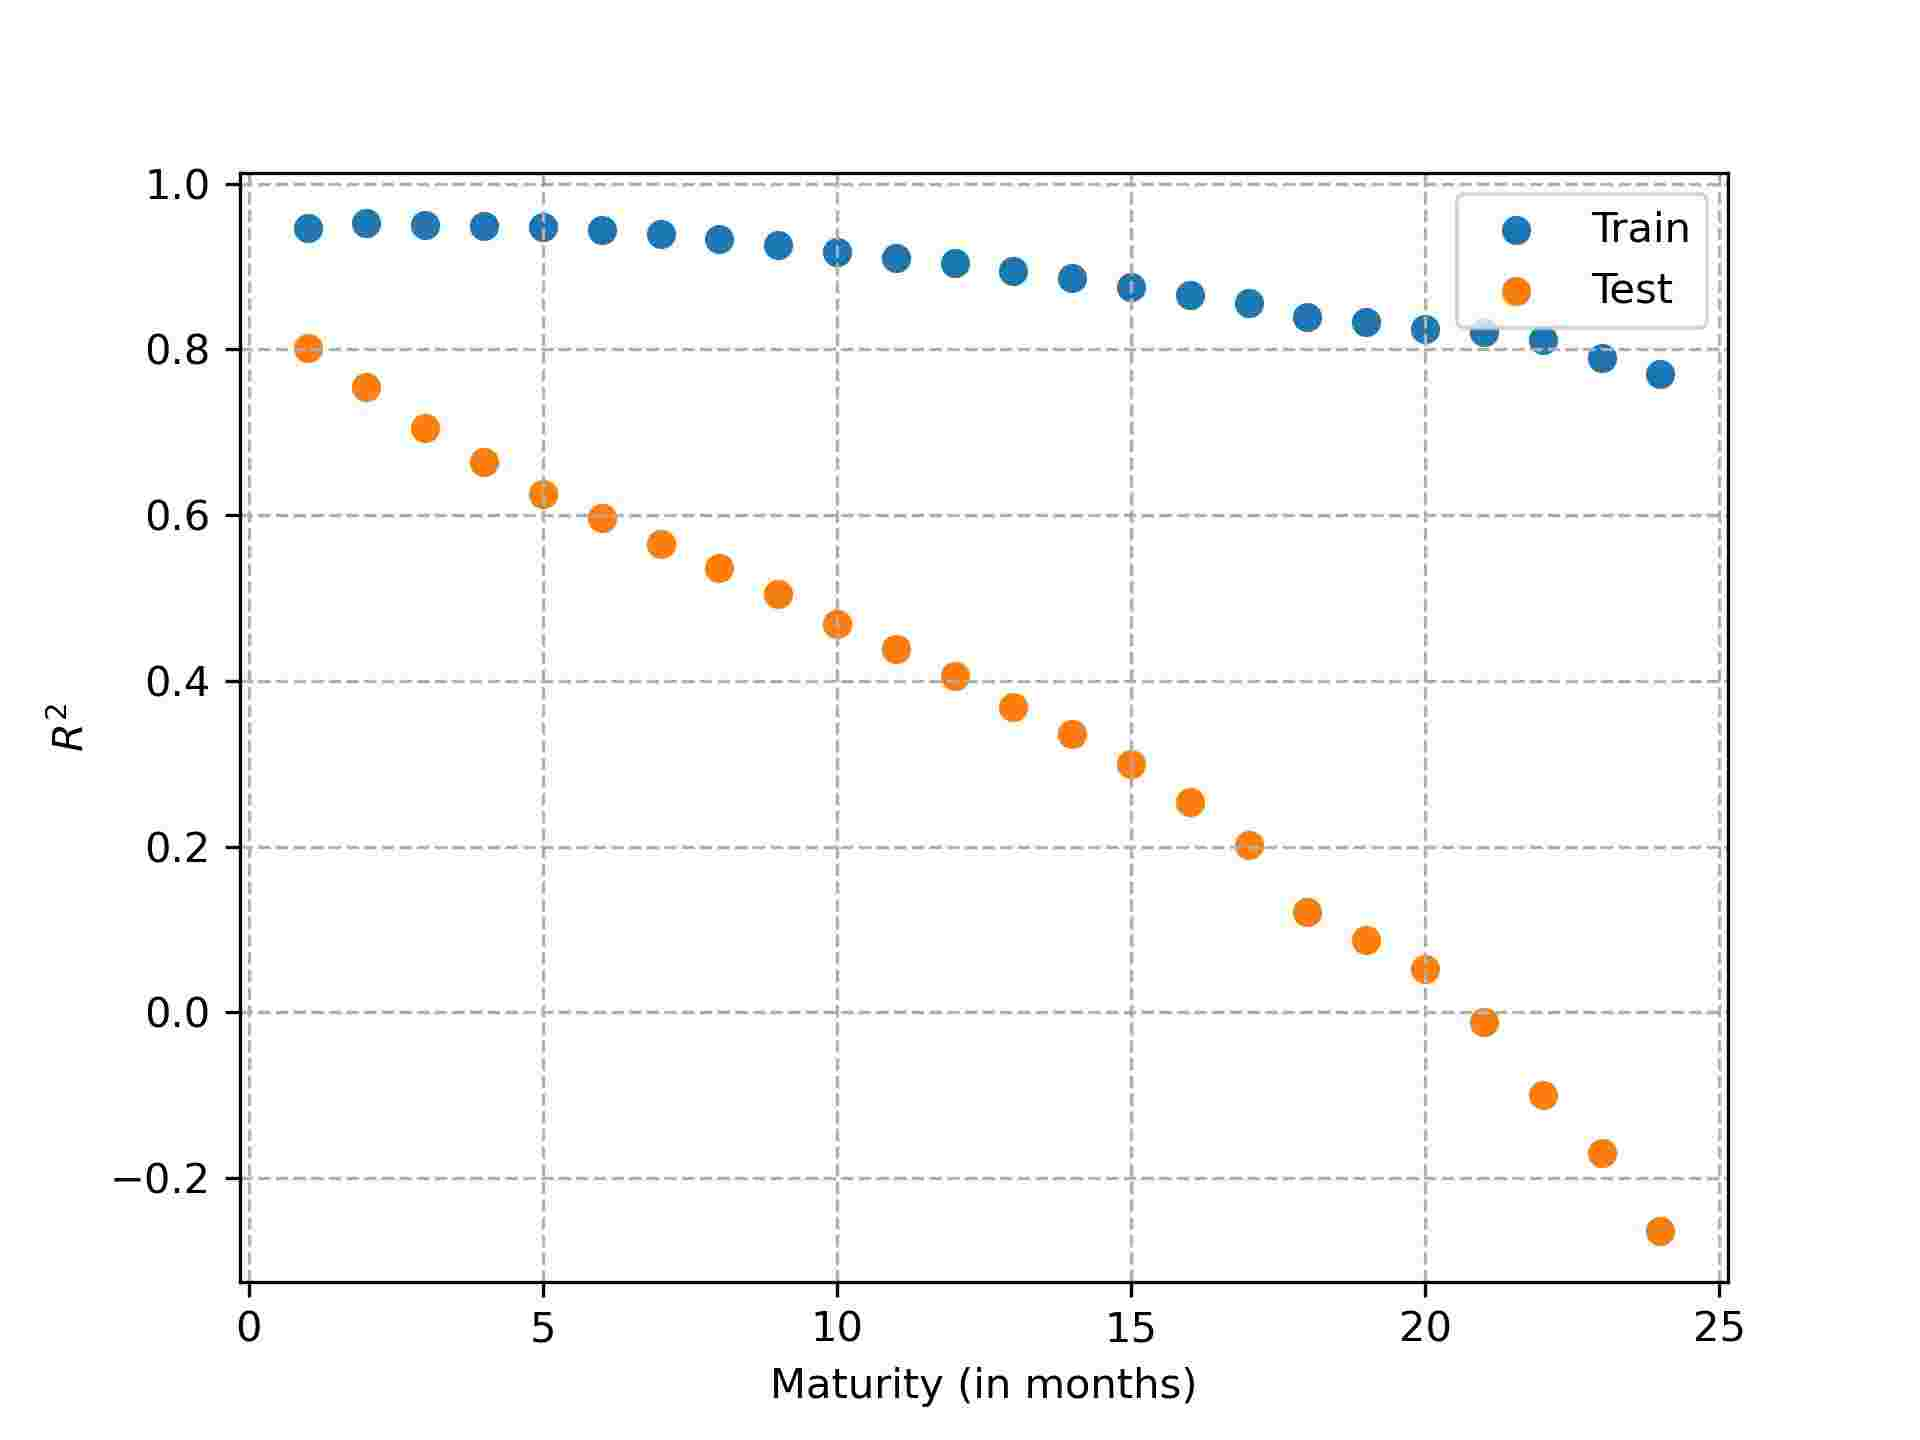
\includegraphics[width=0.45\linewidth]{SPX_Scores_Cutoff_500.jpg}}
    \subfigure[Euro Stoxx 50]{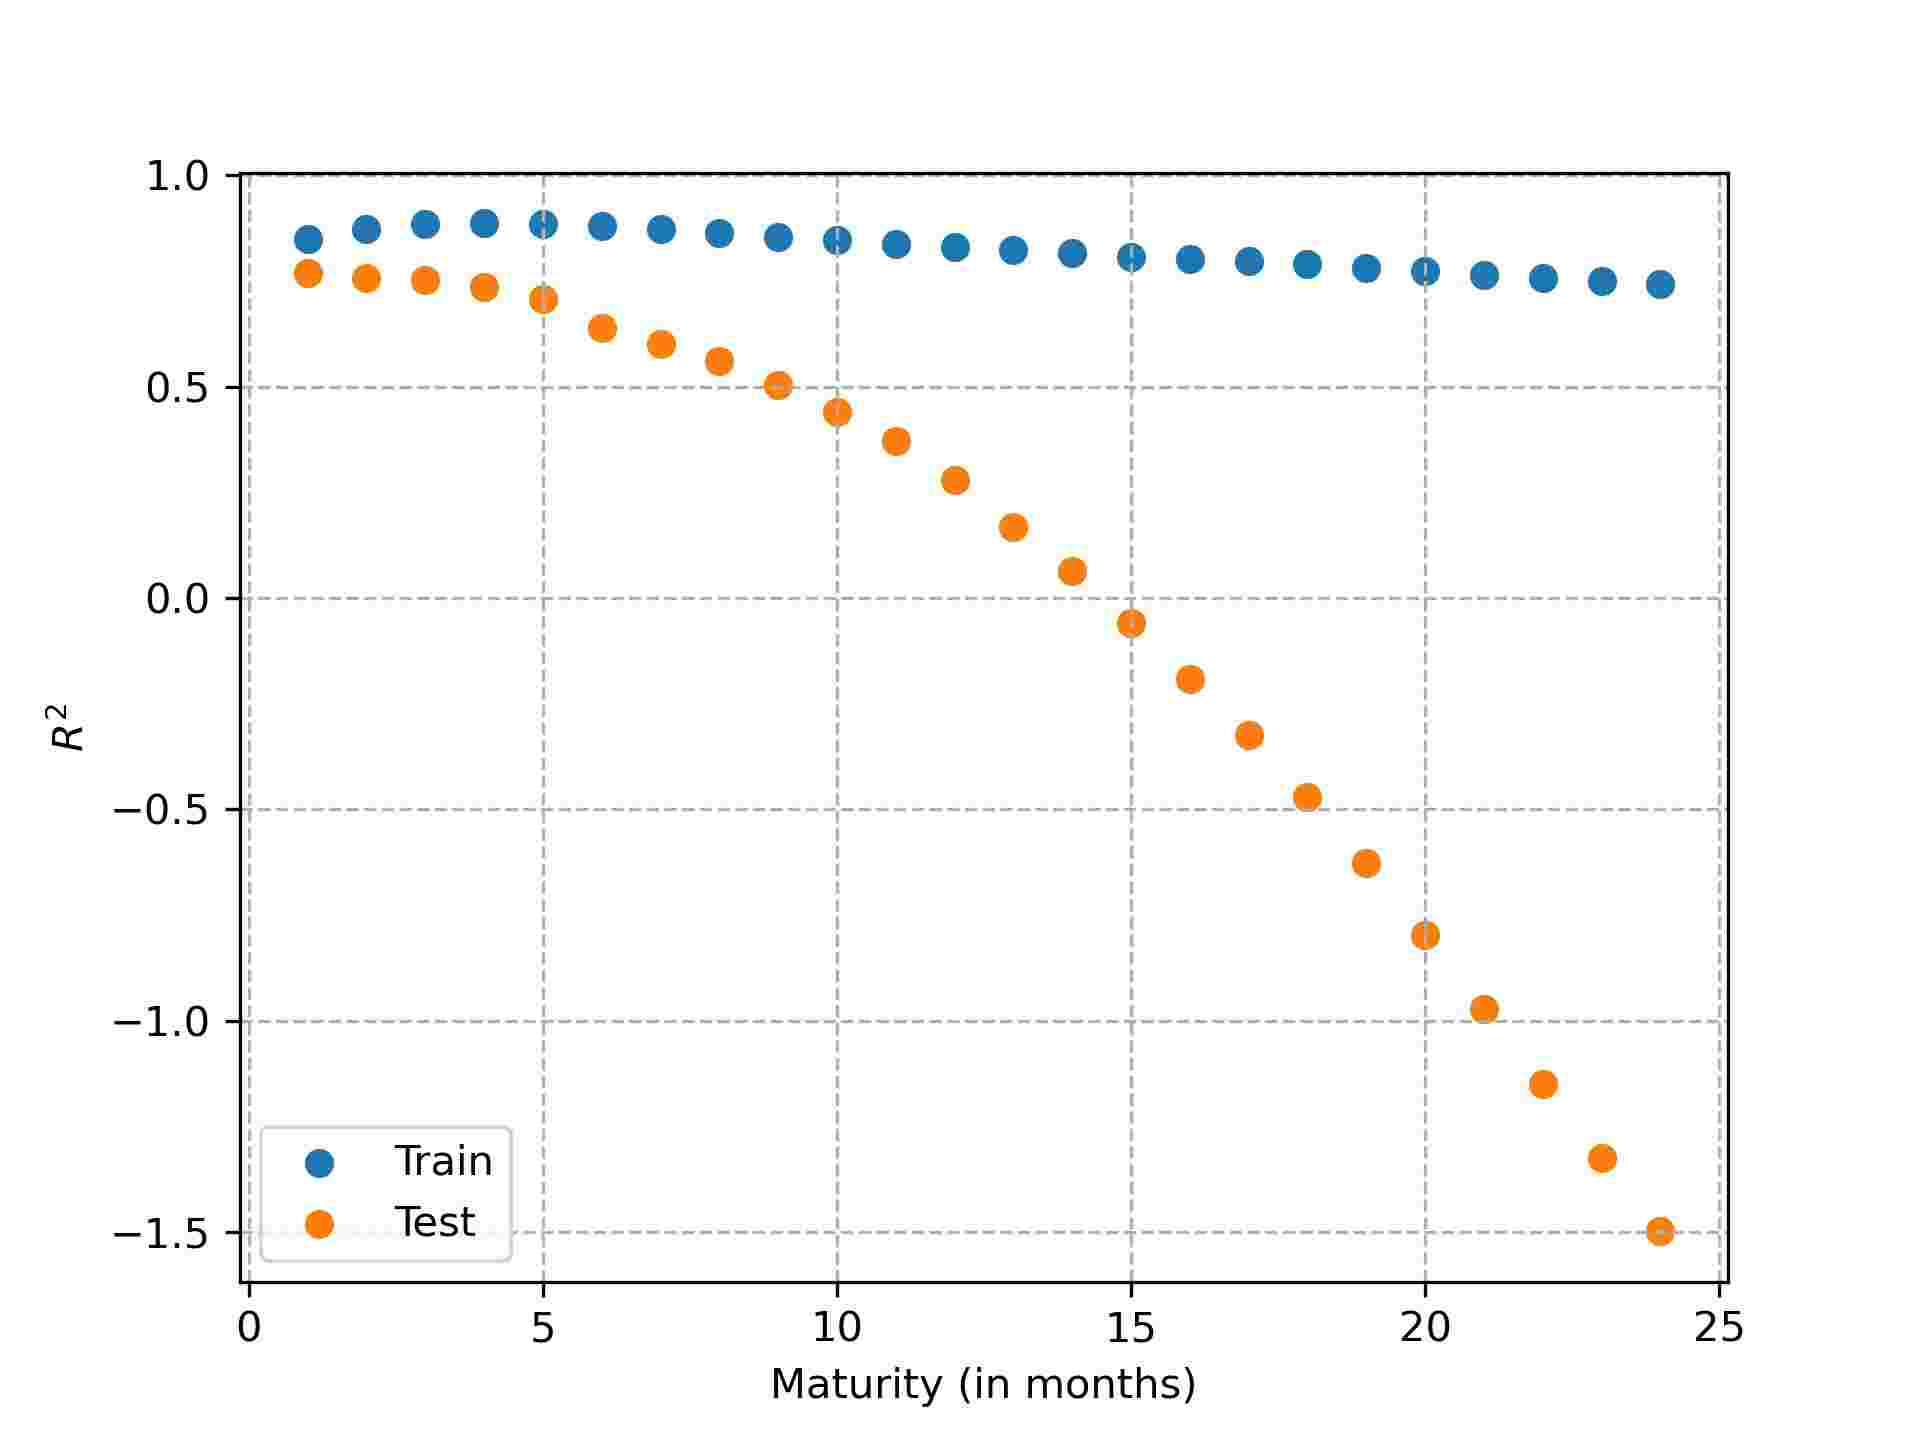
\includegraphics[width=0.45\linewidth]{STXE_Scores_Cutoff_500.jpg}}
    \caption{$R^2$ scores on the train and the test sets as a function of the ATM implied volatility time-to-maturity for $C_{R_1}=C_{\Sigma}=500$ and $\lambda=0$.}
\label{fig:r2_cutoff_500}
\end{figure}

In order to verify that this conclusion is not an artefact of a bad model calibration, we present in Figure \ref{fig:corr_structure} the correlation between the implied variance and the squared daily returns for all lags between 0 and 3,000 days both on the train and the test sets. Note that the estimated correlation $\rho$ is presented along with a 95\% confidence interval derived from the transformation $z=\text{artanh}(\rho)$ introduced by \cite{fisher1915frequency}. Indeed, this transformation is approximately normally distributed when the samples come from a bivariate normal distribution. Although this is not the case here, we consider it as a reasonable proxy of the uncertainty around the correlation estimator. On the train set (blue curve), the graphs show a slow decrease of the correlation with the lag and the decrease becomes slower when the time-to-maturity increases. For the Euro Stoxx 50, we can even observe some spikes at some specific lags that become larger when the time-to-maturity increases. These observations are consistent with the sensitivity of the model to the cut-off lag $C_{\Sigma}$ and the values obtained with the cross-validation that are presented in Table \ref{tab:best_triplets}. Note that these observations have the advantage of not depending on any assumption. Thus, we can consider the long-range dependence of the implied volatility to the past squared returns as a stylized fact of our implied volatility data. An empirical study of a larger set of underlying assets could reveal whether this is a universal property of implied volatility data. To our knowledge, this stylized fact has never been reported in the literature. Let us however mention the work of \cite{hardle2007long} who calibrate a 3-factor model on implied volatility data and show a long-range dependence in the level and absolute returns of the factors loading series. A possible explanation of this phenomenon is that options on widespread equity indices and with relatively large time-to-maturities are presumably traded by long-term investors such as asset managers, pension funds, sovereign funds, etc. who have a low rebalancing frequency of their portfolios and consequently, who base their investment decisions on the previous years returns of the underlying asset rather than the previous days returns. On the other hand, options with shorter time-to-maturities are presumably less traded by long-term investors so that the movements of the implied volatility are more influenced by short-term investors such as hedge funds who base their investment decisions on recent data. This is in line with Figures \ref{fig:1_month_SP500} and \ref{fig:1_month_SX5E} as well as with the smaller values of $C_{\Sigma}$ for the smallest time-to-maturities in Table \ref{tab:best_triplets}. In Figure \ref{fig:corr_structure_r1}, we also present the correlations between the implied volatility and the daily returns for all lags between 0 and 3,000 days both on the train and the test sets. In this case, the correlations fades very quickly with the lag and we do not observe material spikes. \\

So far, we have only described the correlations on the train set but as already discussed extensively, the test set is quite different and the correlations on this set (in orange in Figures \ref{fig:corr_structure} and \ref{fig:corr_structure_r1}) are therefore also distinct from those calculated on the train set. In particular in Figure \ref{fig:corr_structure}, we observe negative correlations with the 250 days lag which can be understood as a consequence of the fact that the implied volatility was decreasing in 2021 due to the leverage effect while one year earlier the squared returns were increasing with the Covid-19 crisis. Conversely, the implied volatility increased in 2022 again due to the leverage effect while one year earlier the squared returns were decreasing with the post-Covid-19 bull market. 

\begin{figure}
    \centering
    \subfigure[1-month ATM implied volatility (S\&P 500)]{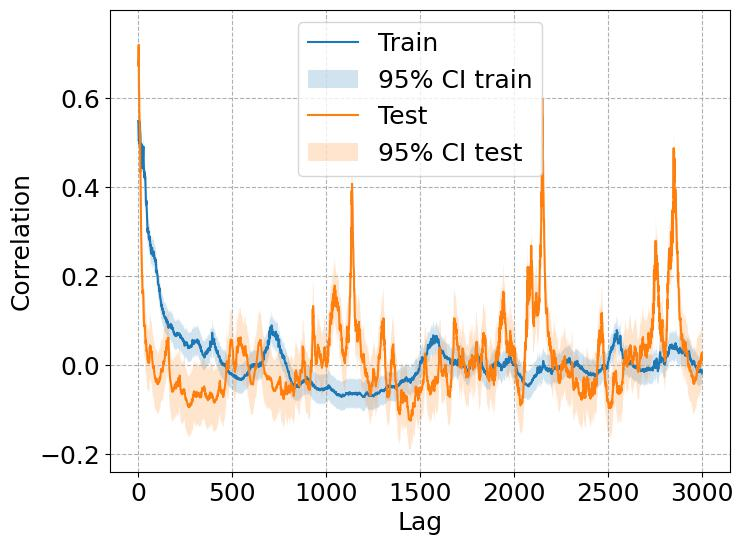
\includegraphics[width=0.3\linewidth]{SPX_1M_R2_Correlation.jpg}\label{fig:1_month_SP500}}
    \subfigure[12-months ATM implied volatility (S\&P 500)]{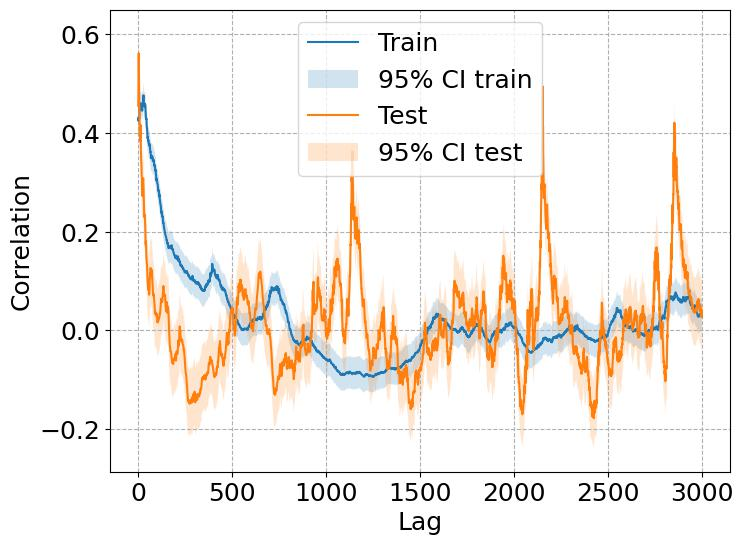
\includegraphics[width=0.3\linewidth]{SPX_12M_R2_Correlation.jpg}}
    \subfigure[24-months ATM implied volatility (S\&P 500)]{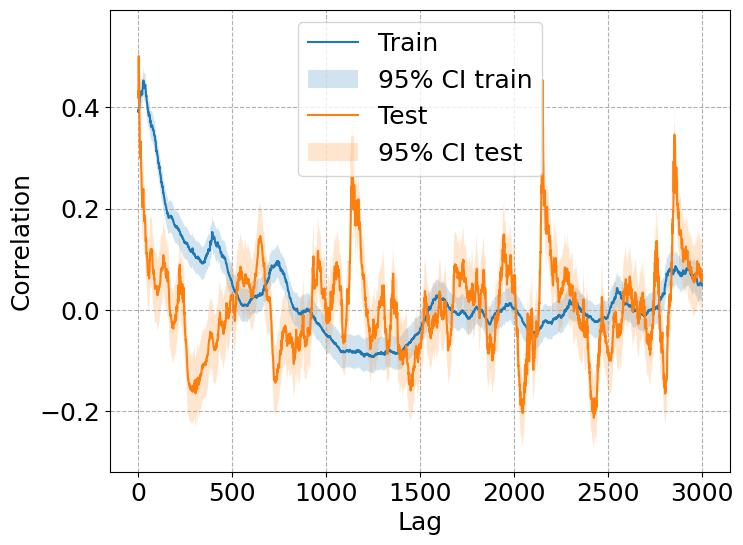
\includegraphics[width=0.3\linewidth]{SPX_24M_R2_Correlation.jpg}}
    \subfigure[1-month ATM implied volatility (Euro Stoxx 50)]{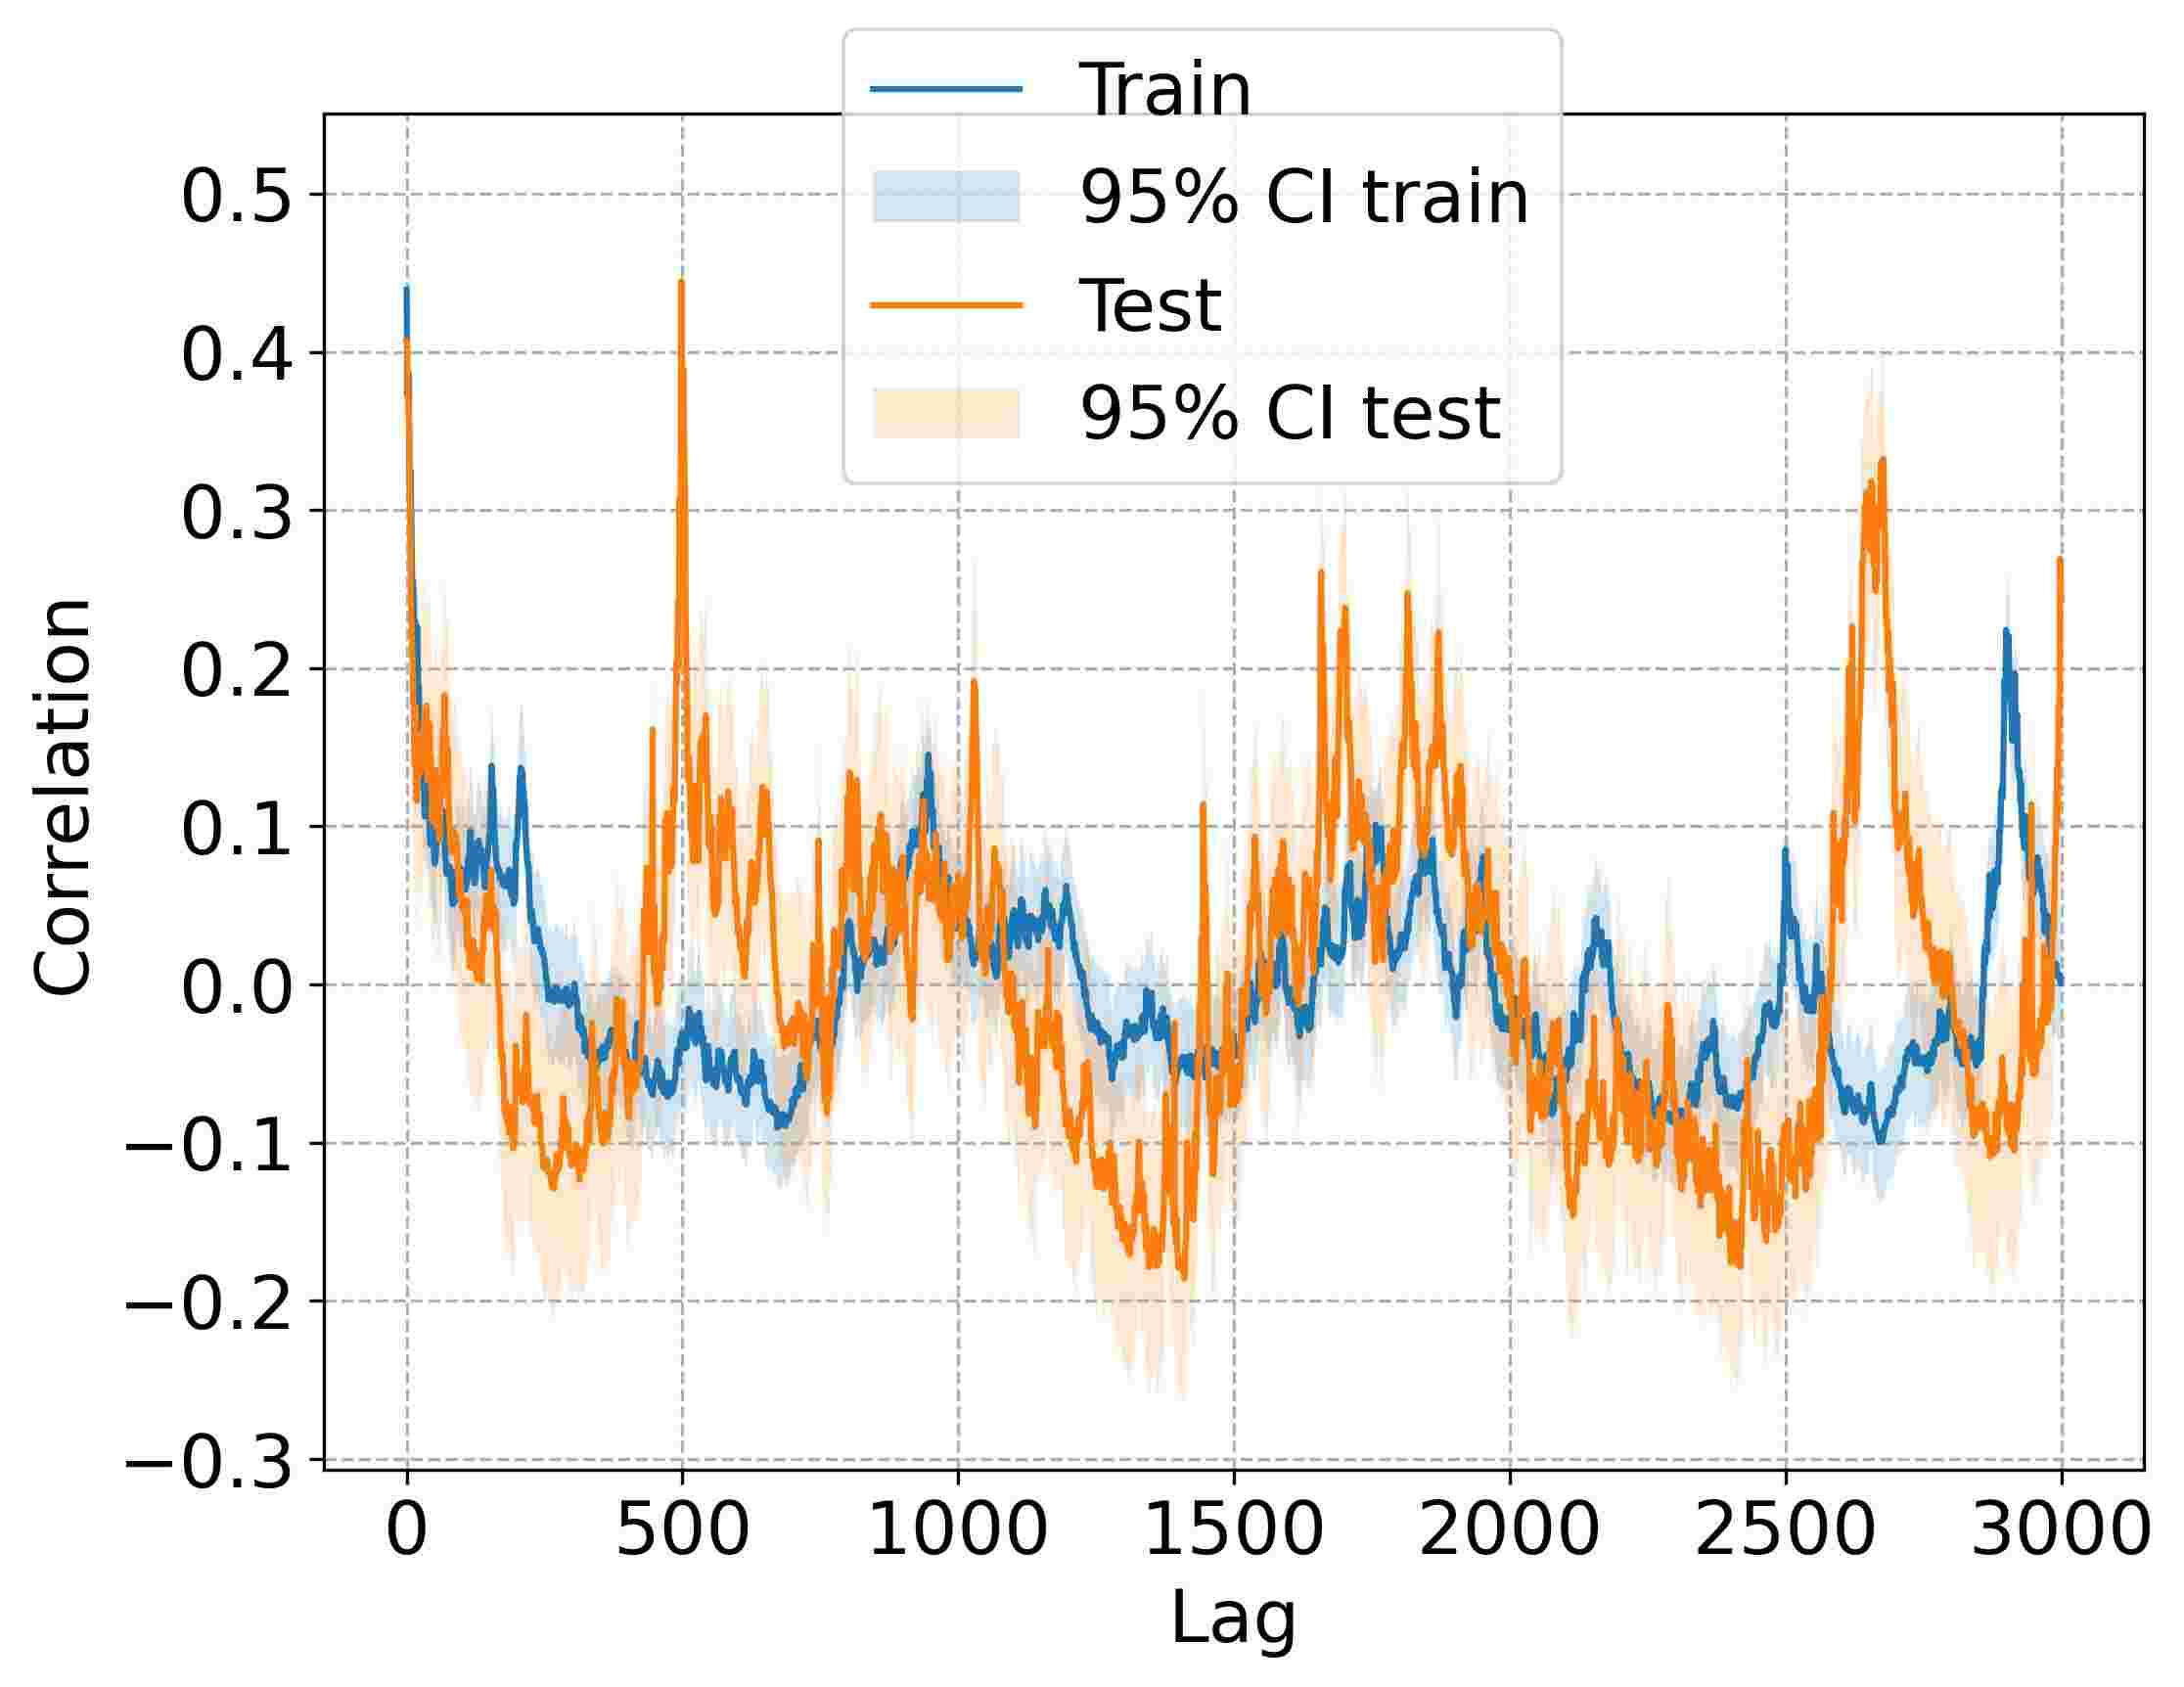
\includegraphics[width=0.3\linewidth]{STXE1MO_R2_Correlation.jpg}\label{fig:1_month_SX5E}}
    \subfigure[12-months ATM implied volatility (Euro Stoxx 50)]{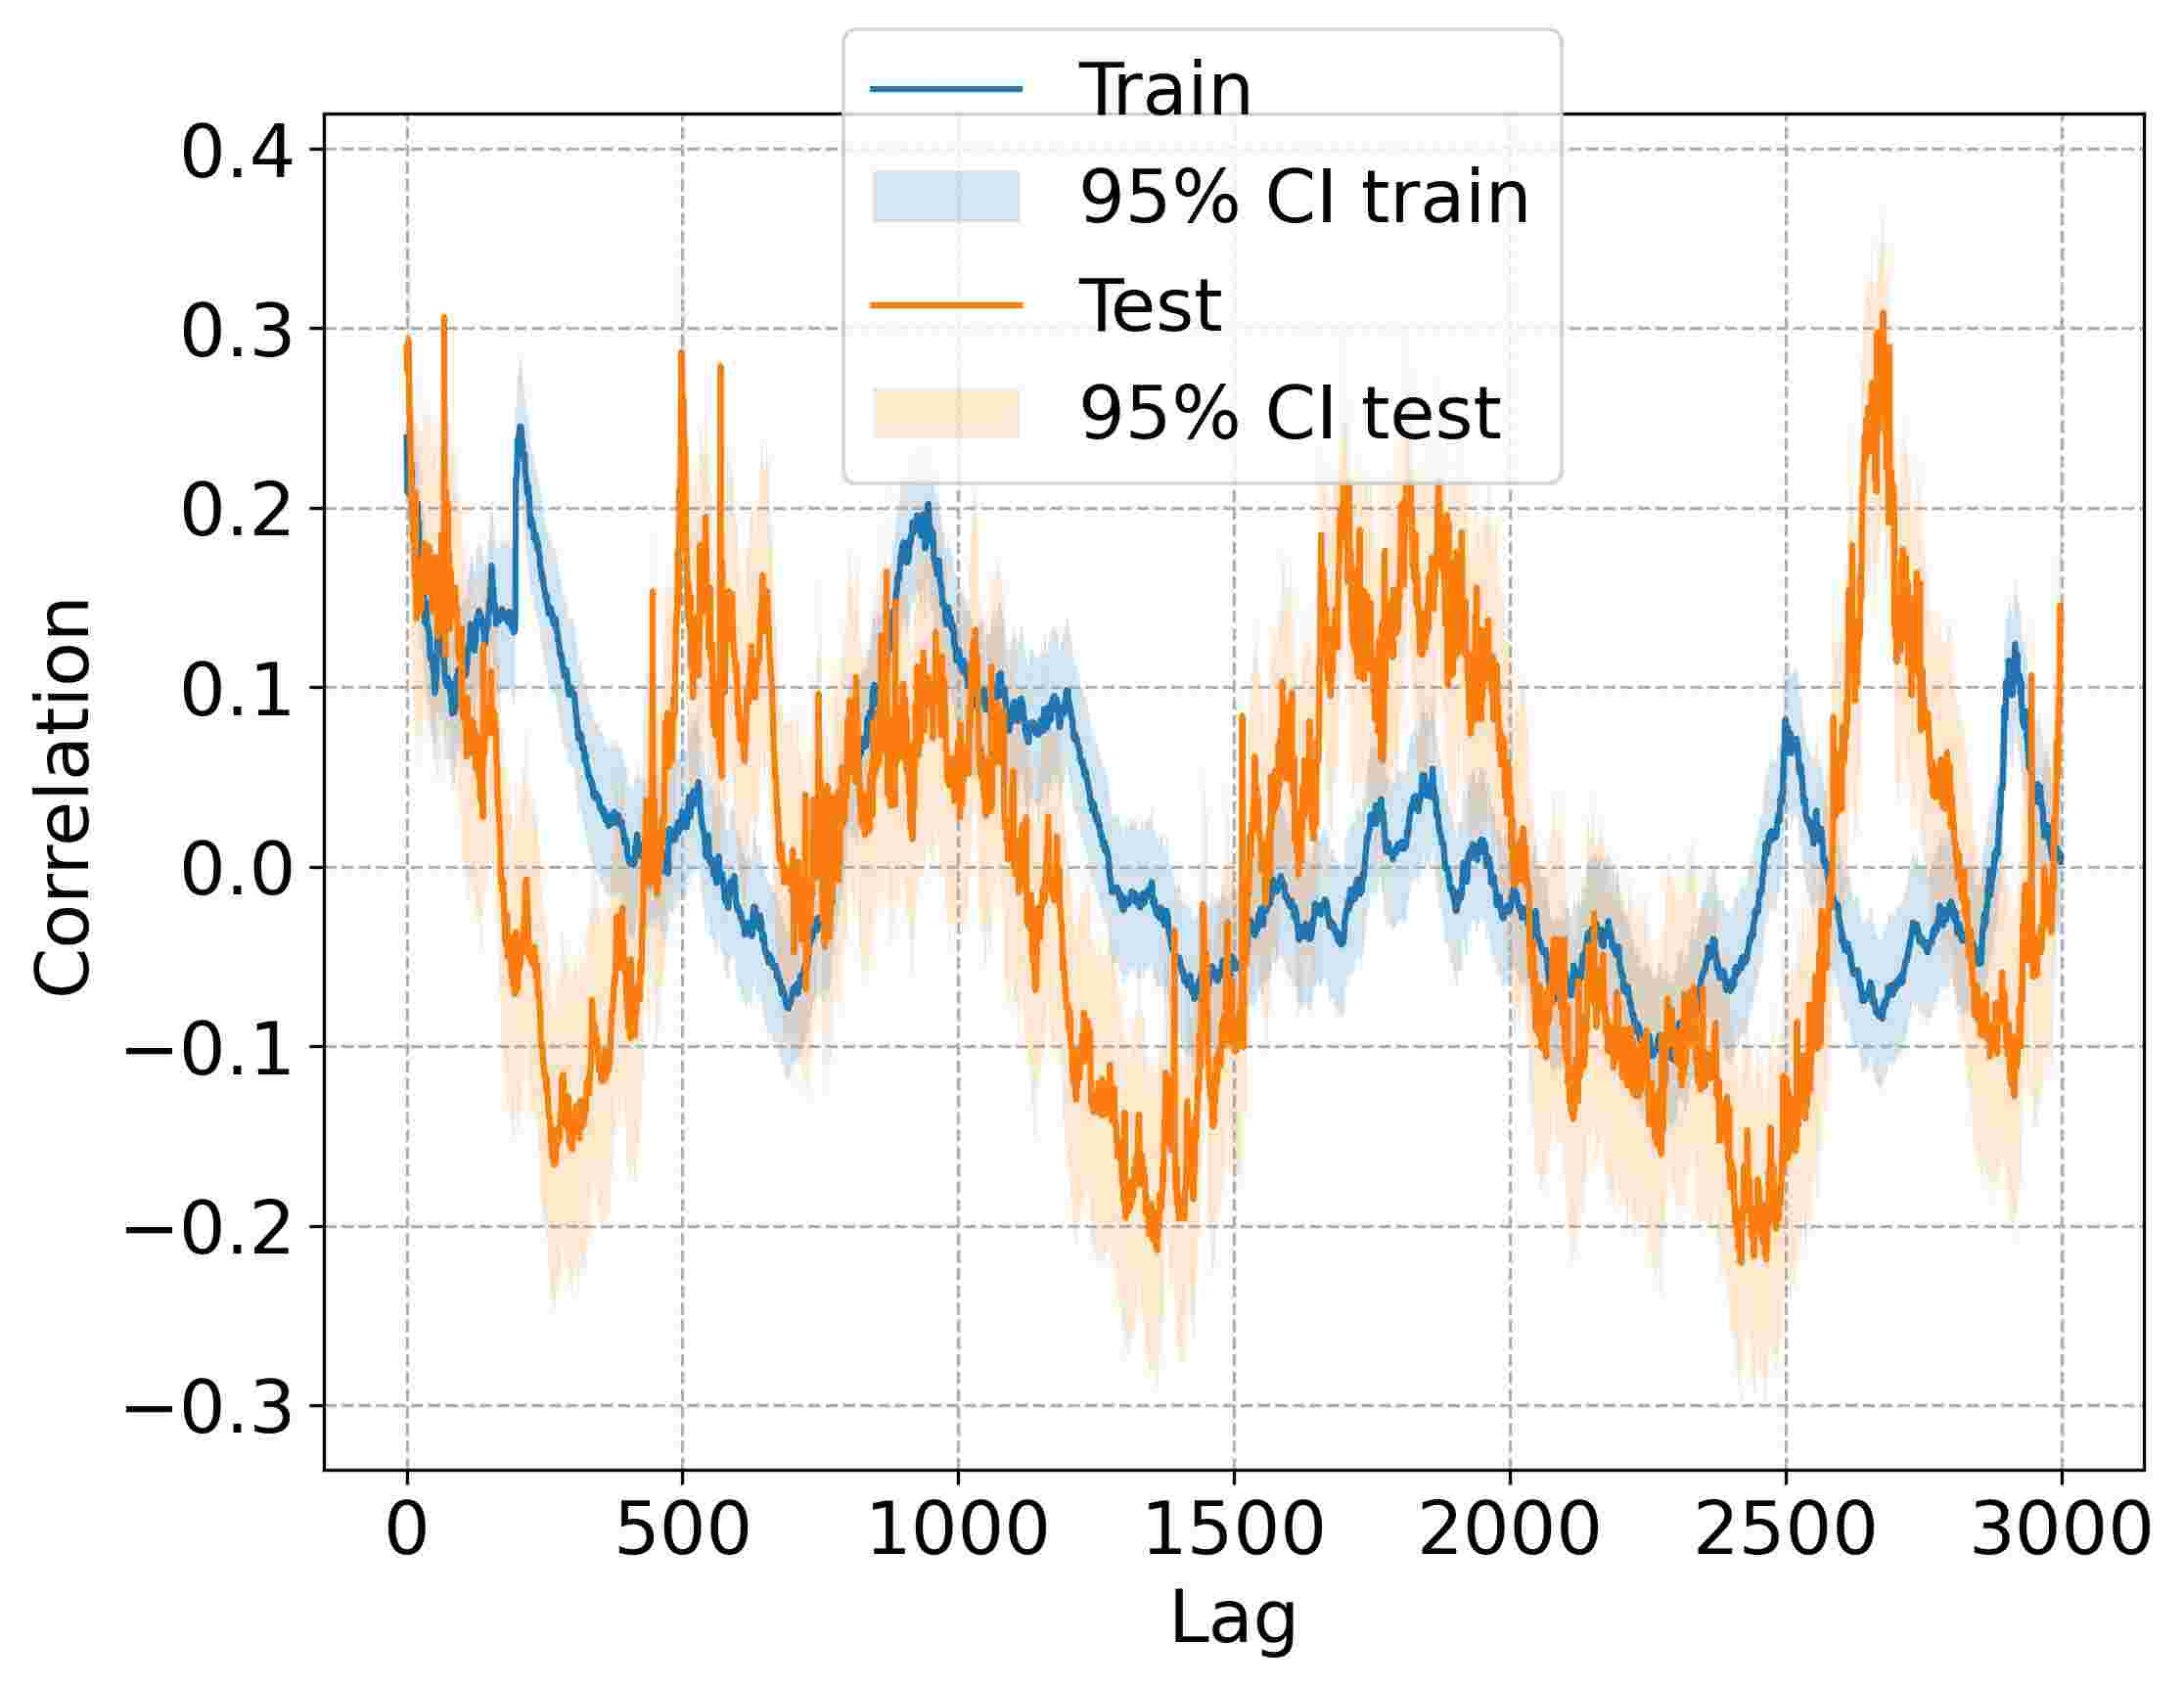
\includegraphics[width=0.3\linewidth]{STXE12MO_R2_Correlation.jpg}}
    \subfigure[24-months ATM implied volatility (Euro Stoxx 50)]{        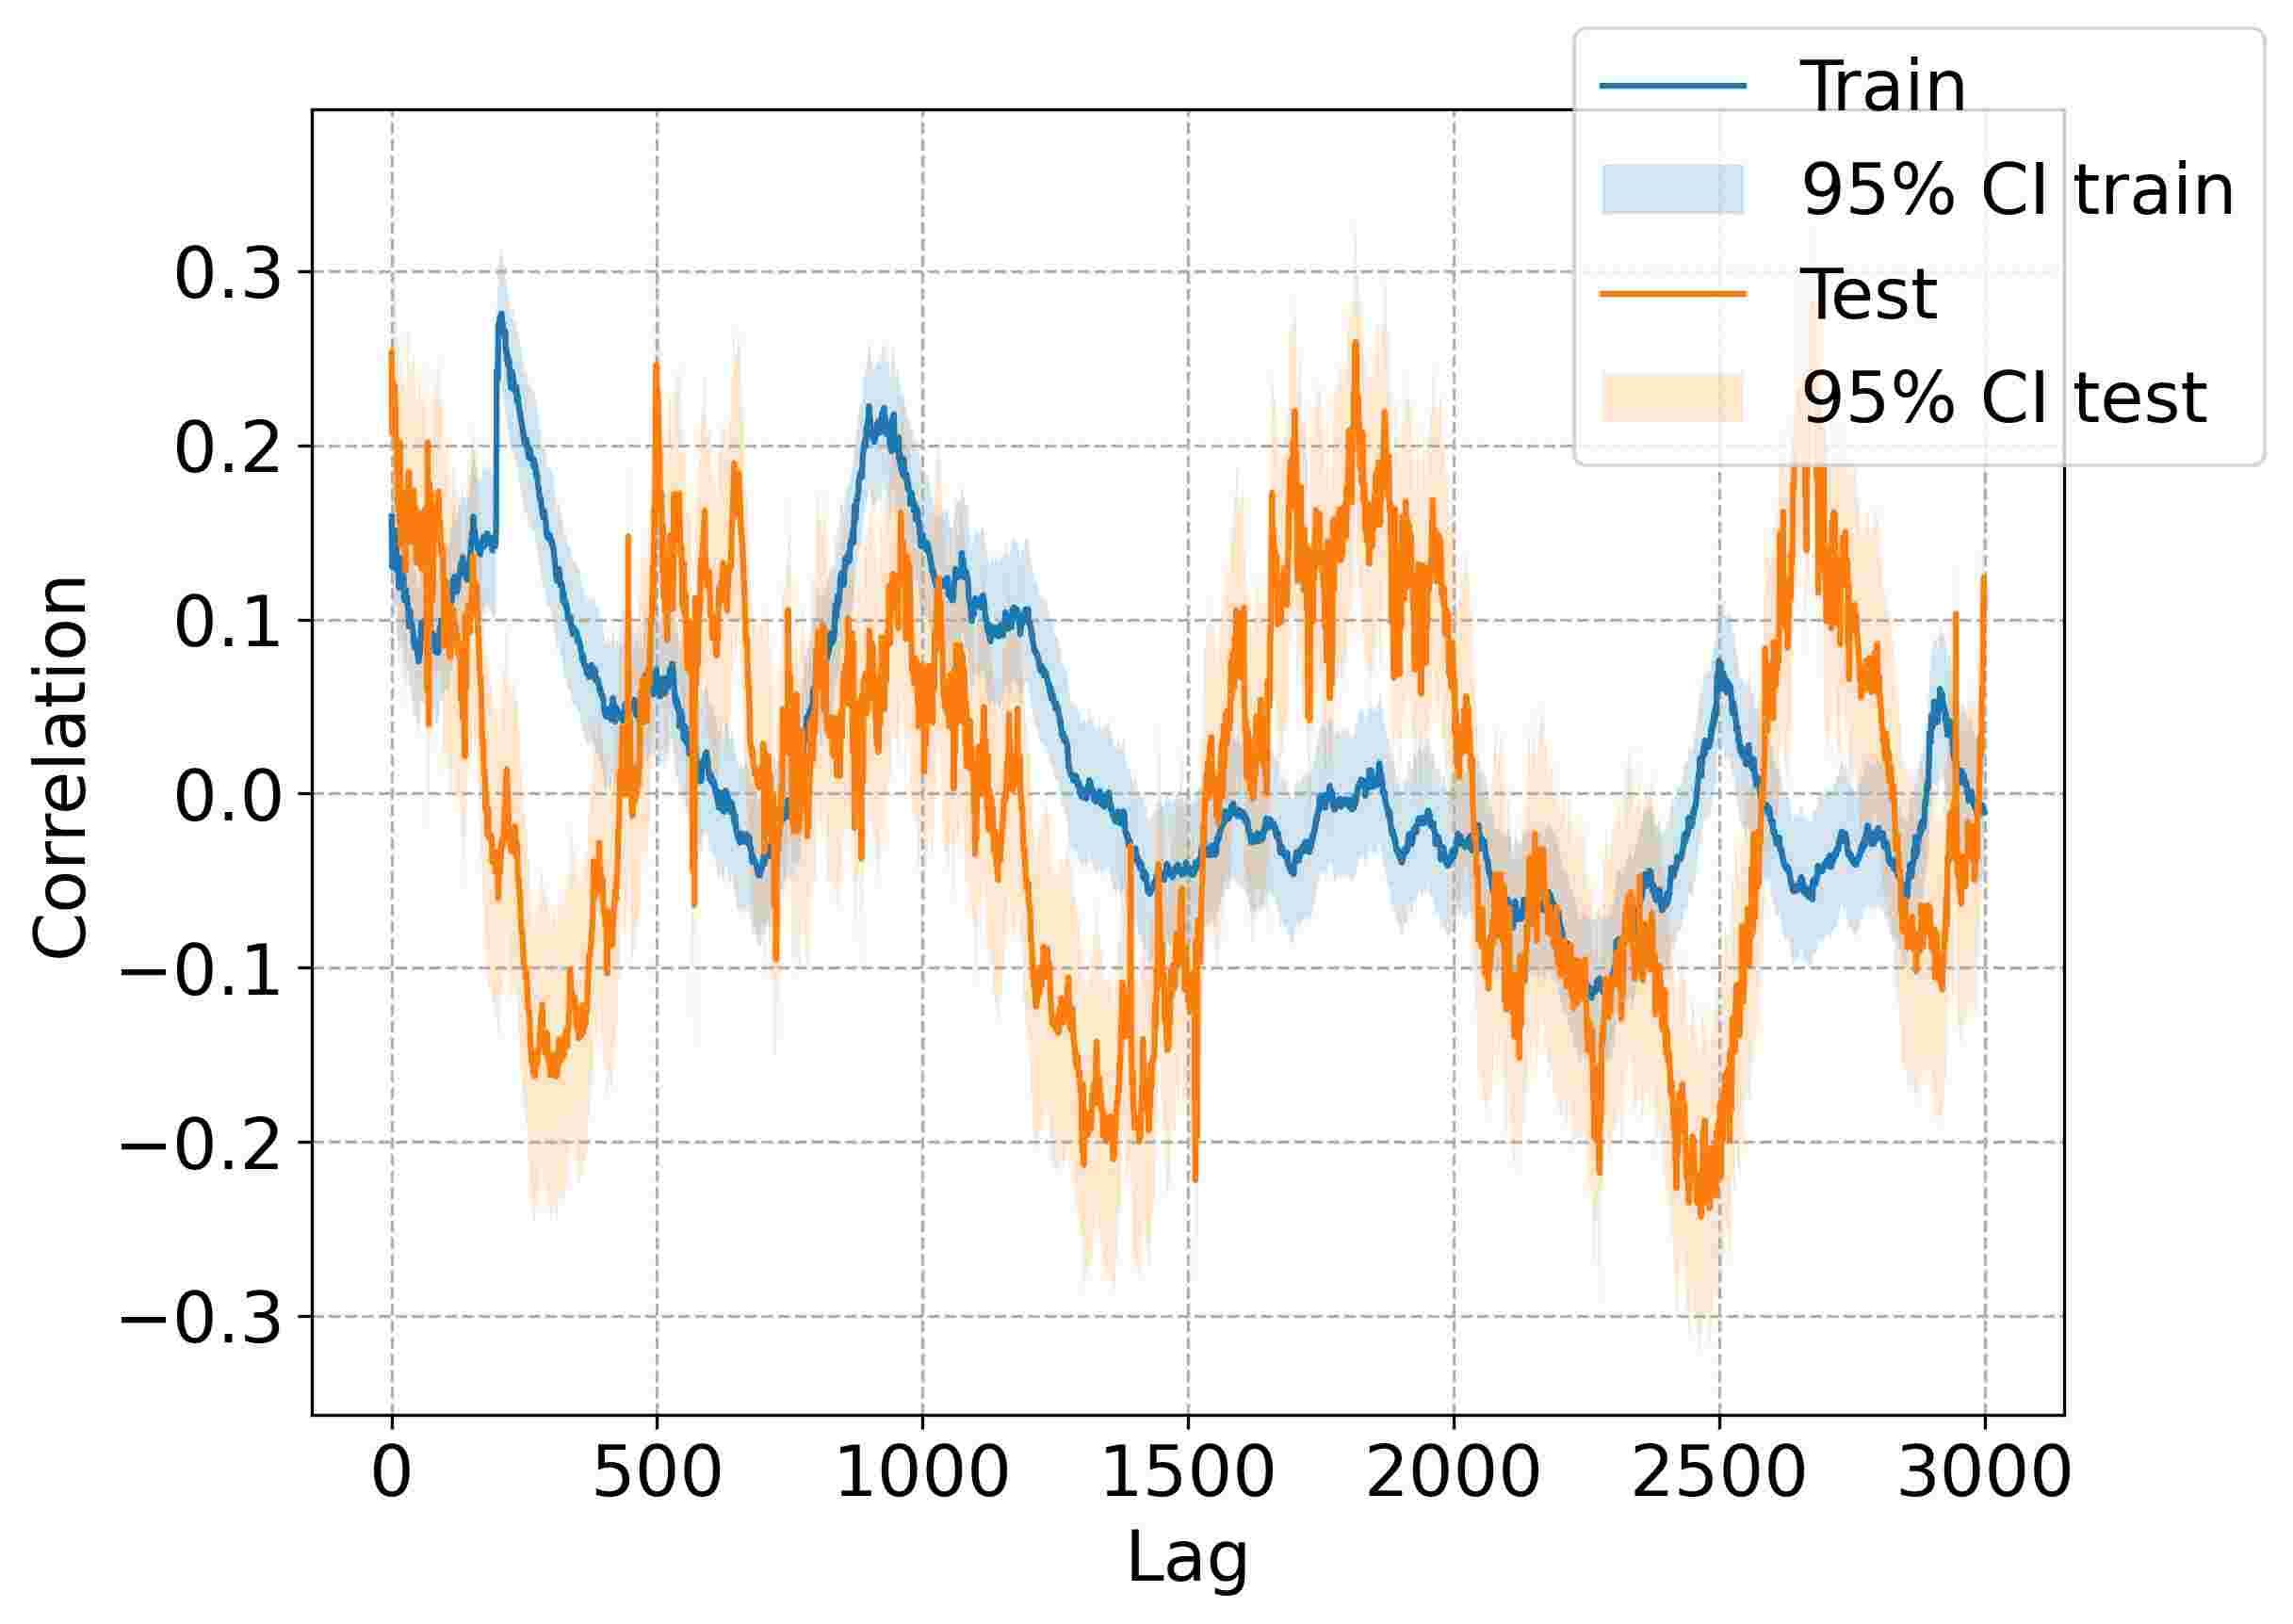
\includegraphics[width=0.3\linewidth]{STXE24MO_R2_Correlation.jpg}}
    \caption{Correlation between the squared ATM implied volatility and the squared daily returns as a function of the lag both on the train and the test sets. The 95\% confidence intervals are derived from the Fisher transformation. }
\label{fig:corr_structure}
\end{figure}


\begin{figure}
    \centering
    \subfigure[1-month ATM implied volatility (S\&P 500)]{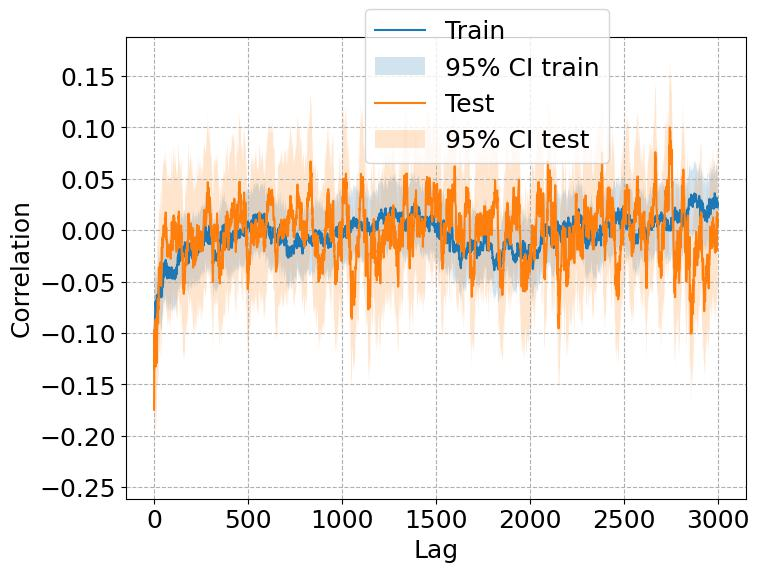
\includegraphics[width=0.3\linewidth]{SPX_1M_R1_Correlation.jpg}}
    \subfigure[12-months ATM implied volatility (S\&P 500)]{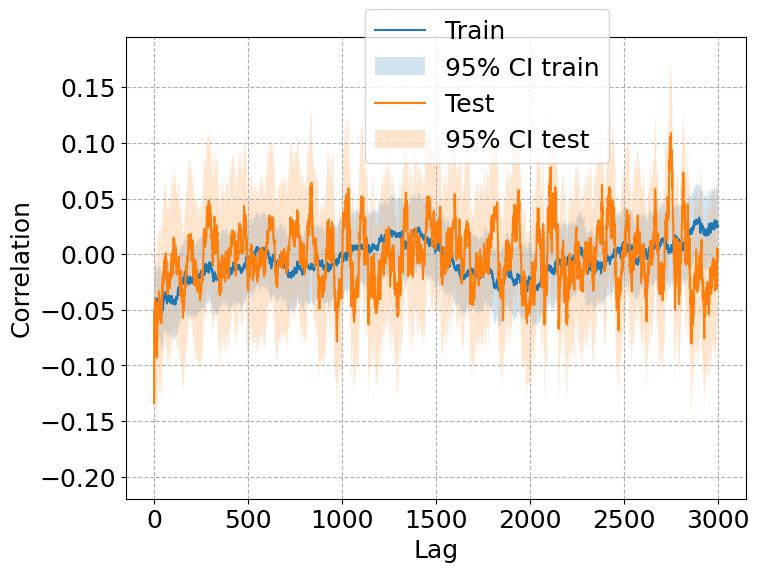
\includegraphics[width=0.3\linewidth]{SPX_12M_R1_Correlation.jpg}}
    \subfigure[24-months ATM implied volatility (S\&P 500)]{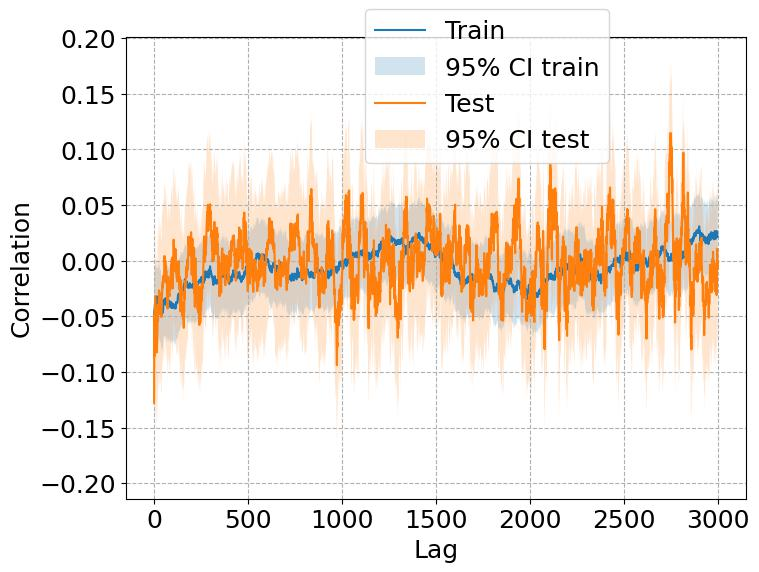
\includegraphics[width=0.3\linewidth]{SPX_24M_R1_Correlation.jpg}}
    \subfigure[1-month ATM implied volatility (Euro Stoxx 50)]{ 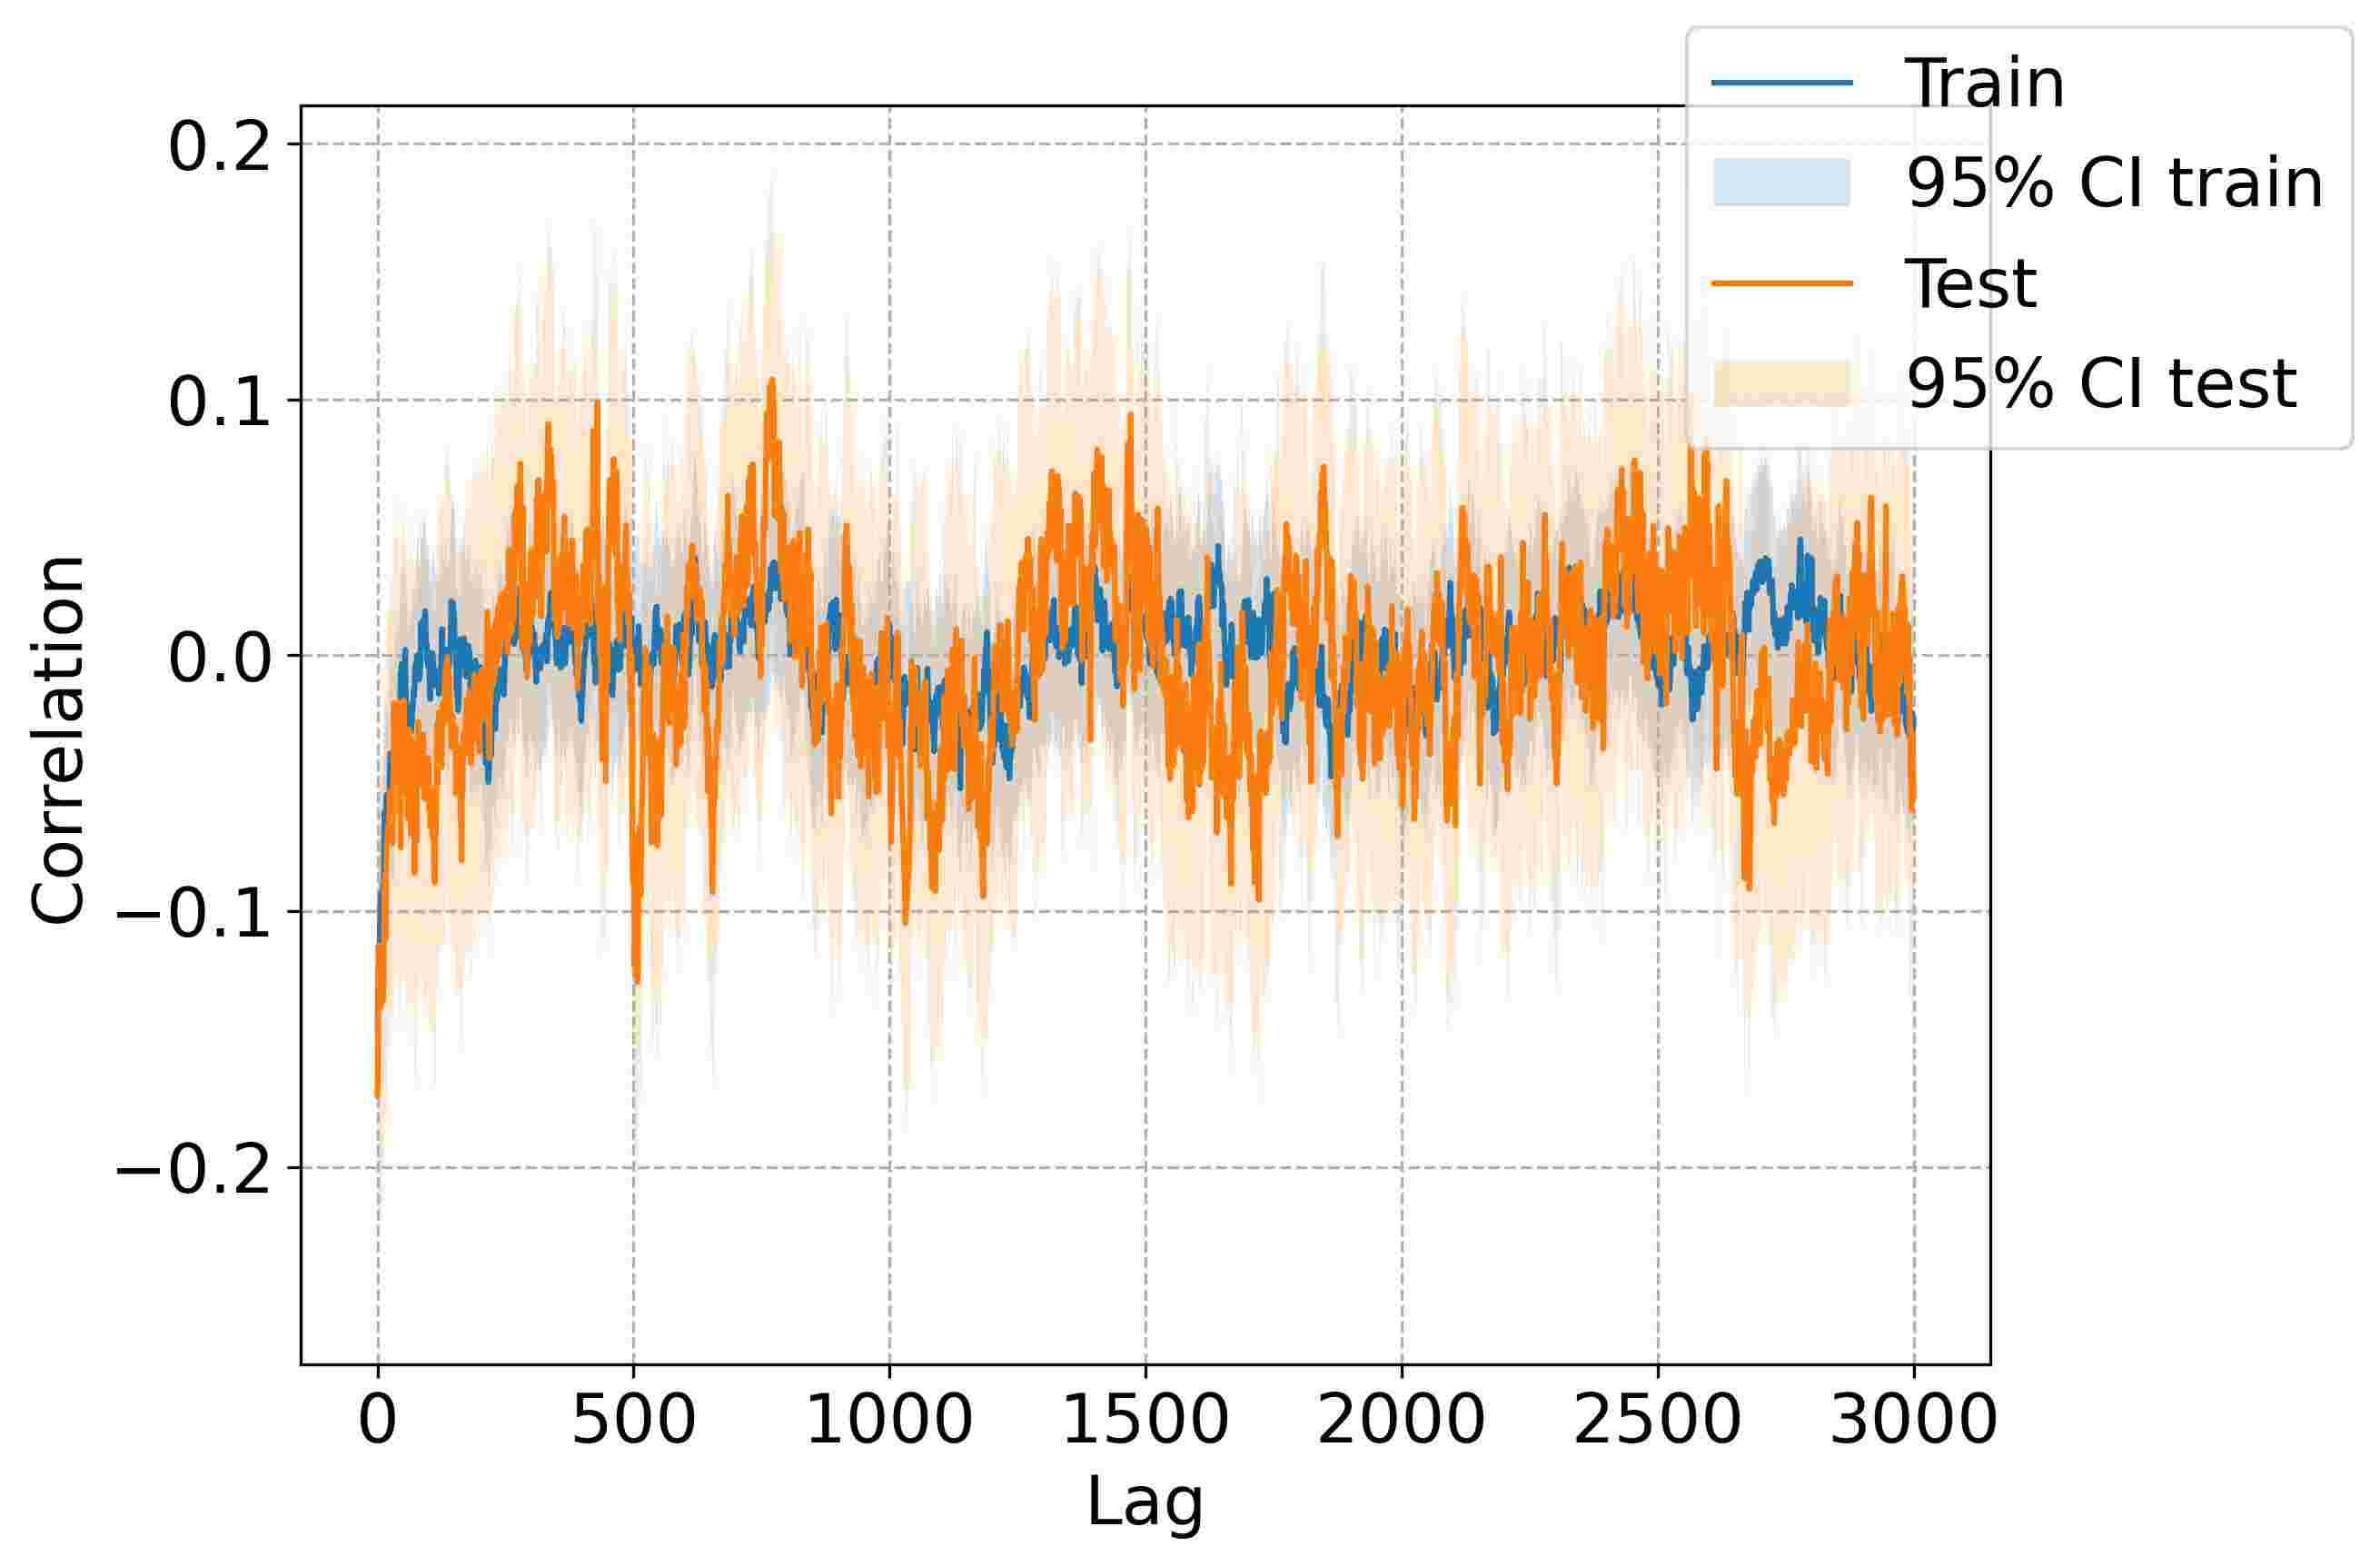
\includegraphics[width=0.3\linewidth]{STXE1MO_R1_Correlation.jpg}}
    \subfigure[12-months ATM implied volatility (Euro Stoxx 50)]{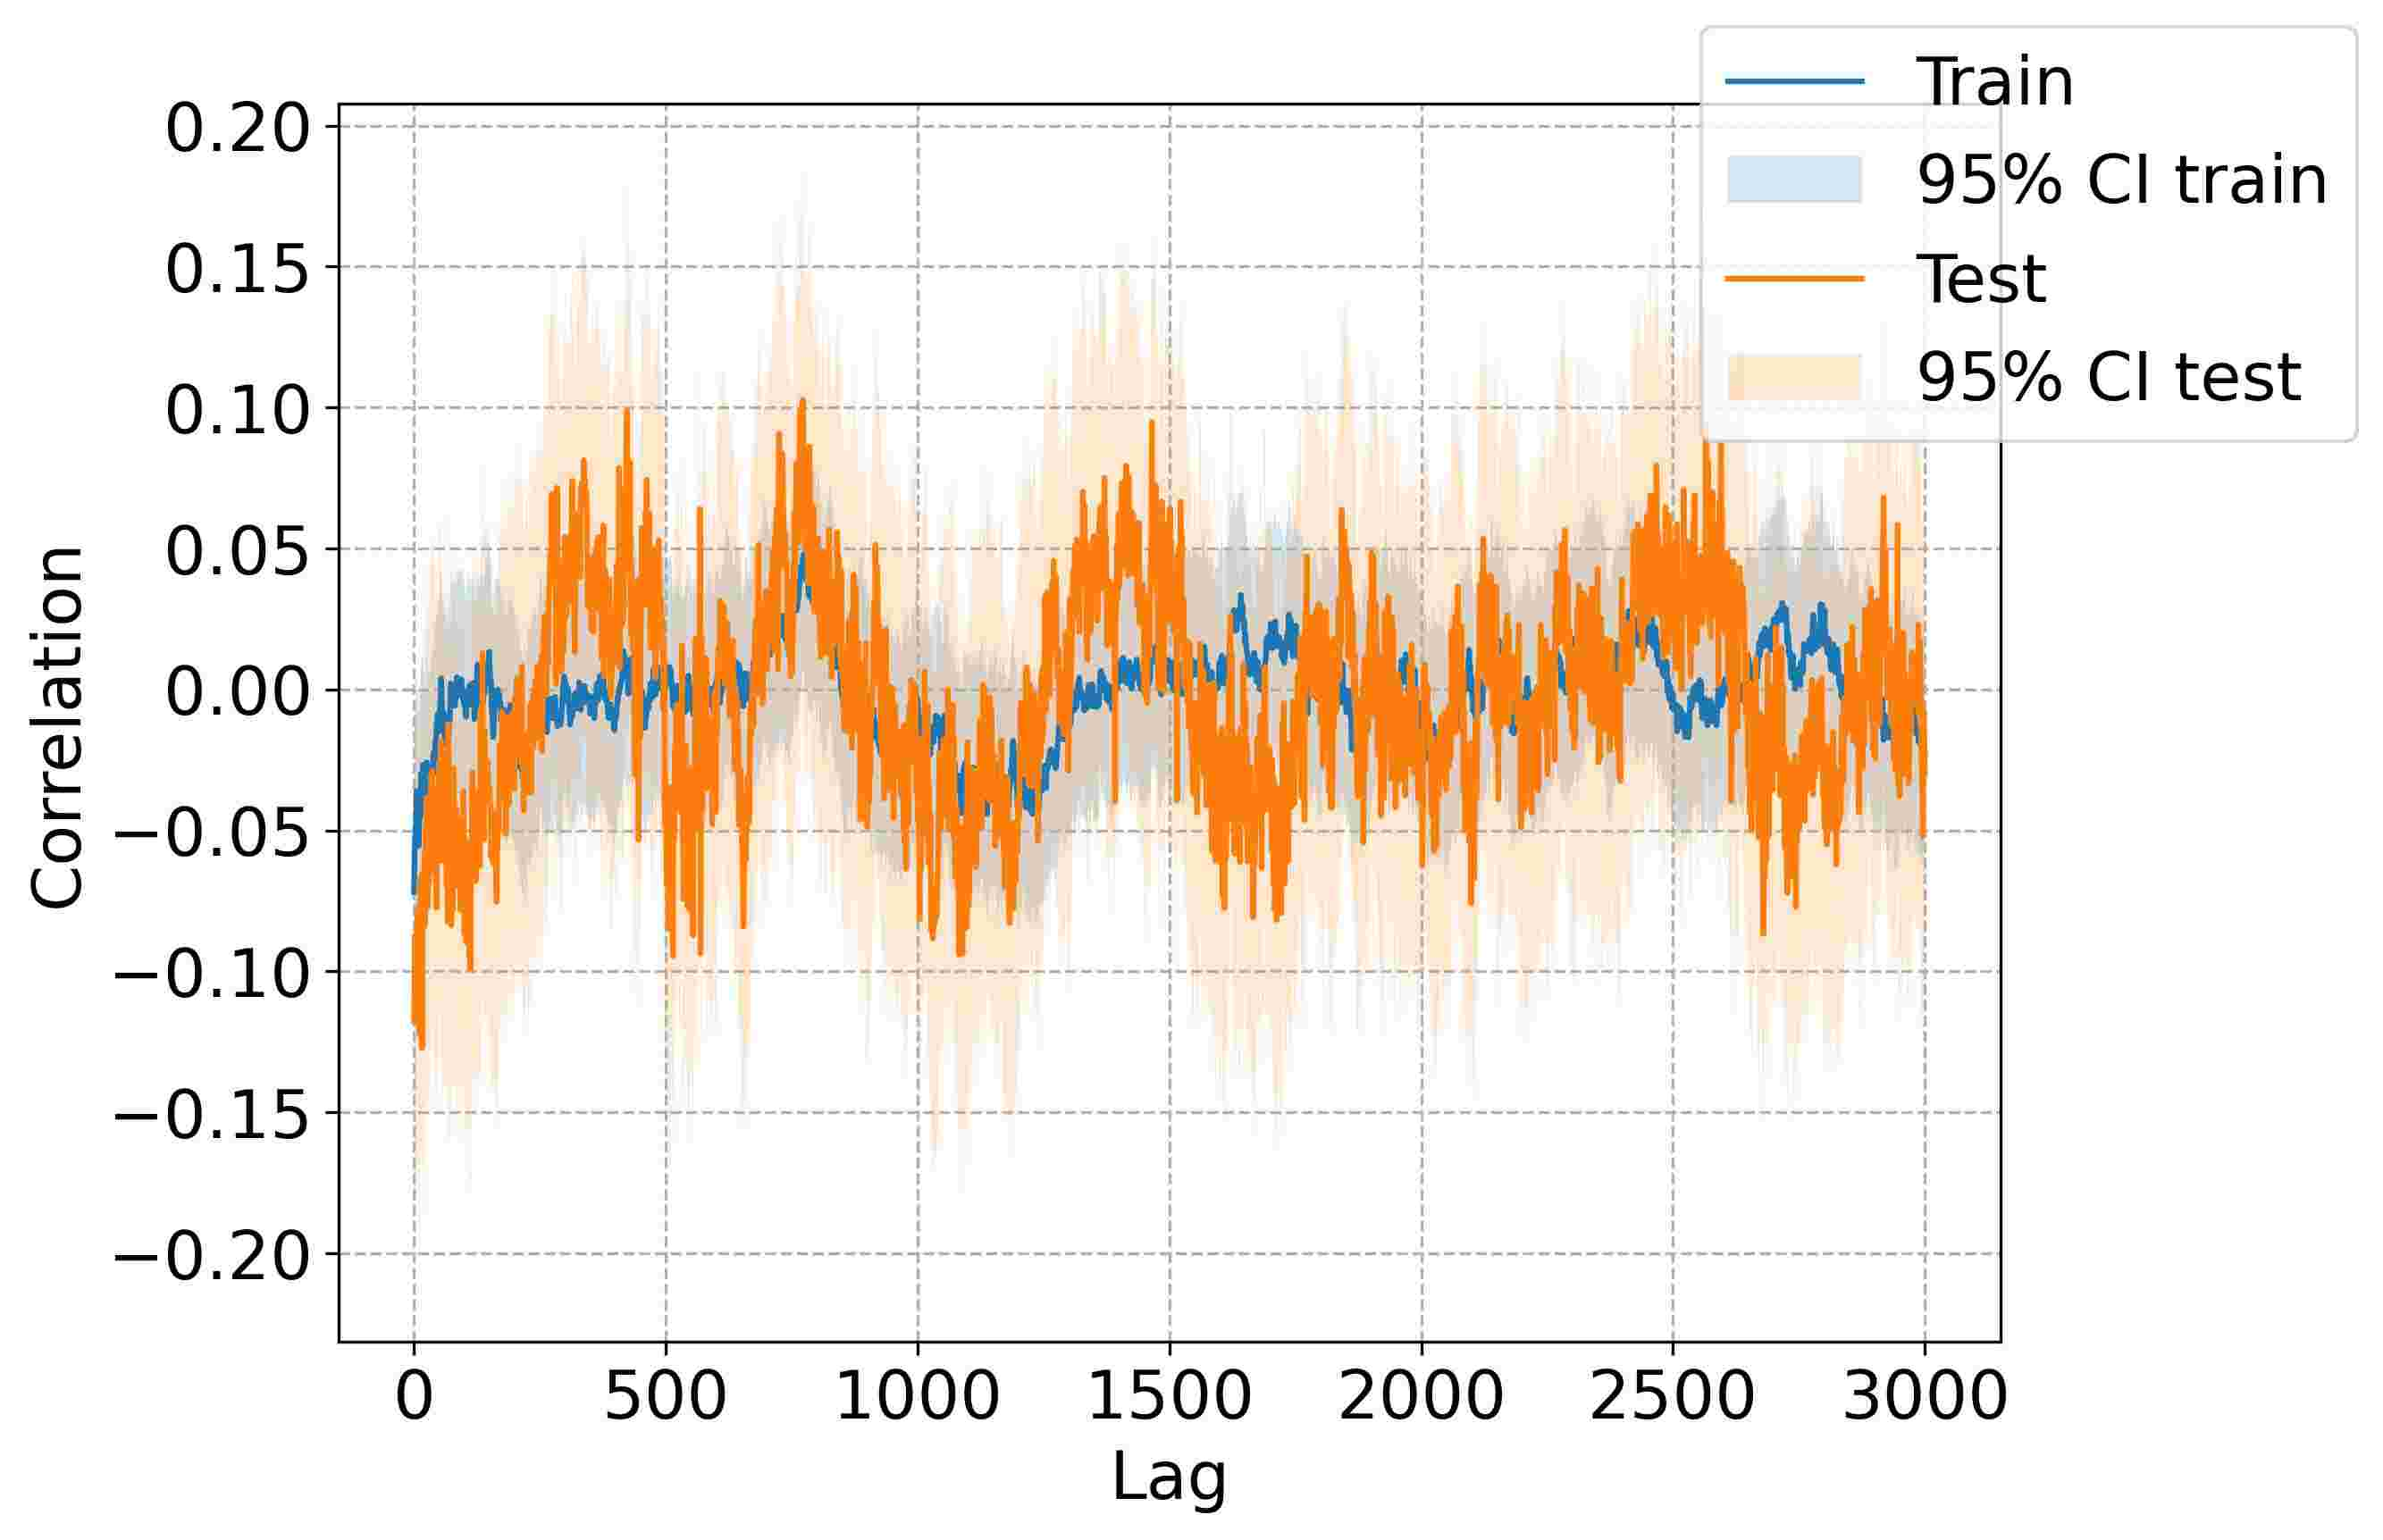
\includegraphics[width=0.3\linewidth]{STXE12MO_R1_Correlation.jpg}}
    \subfigure[24-months ATM implied volatility (Euro Stoxx 50) ]{        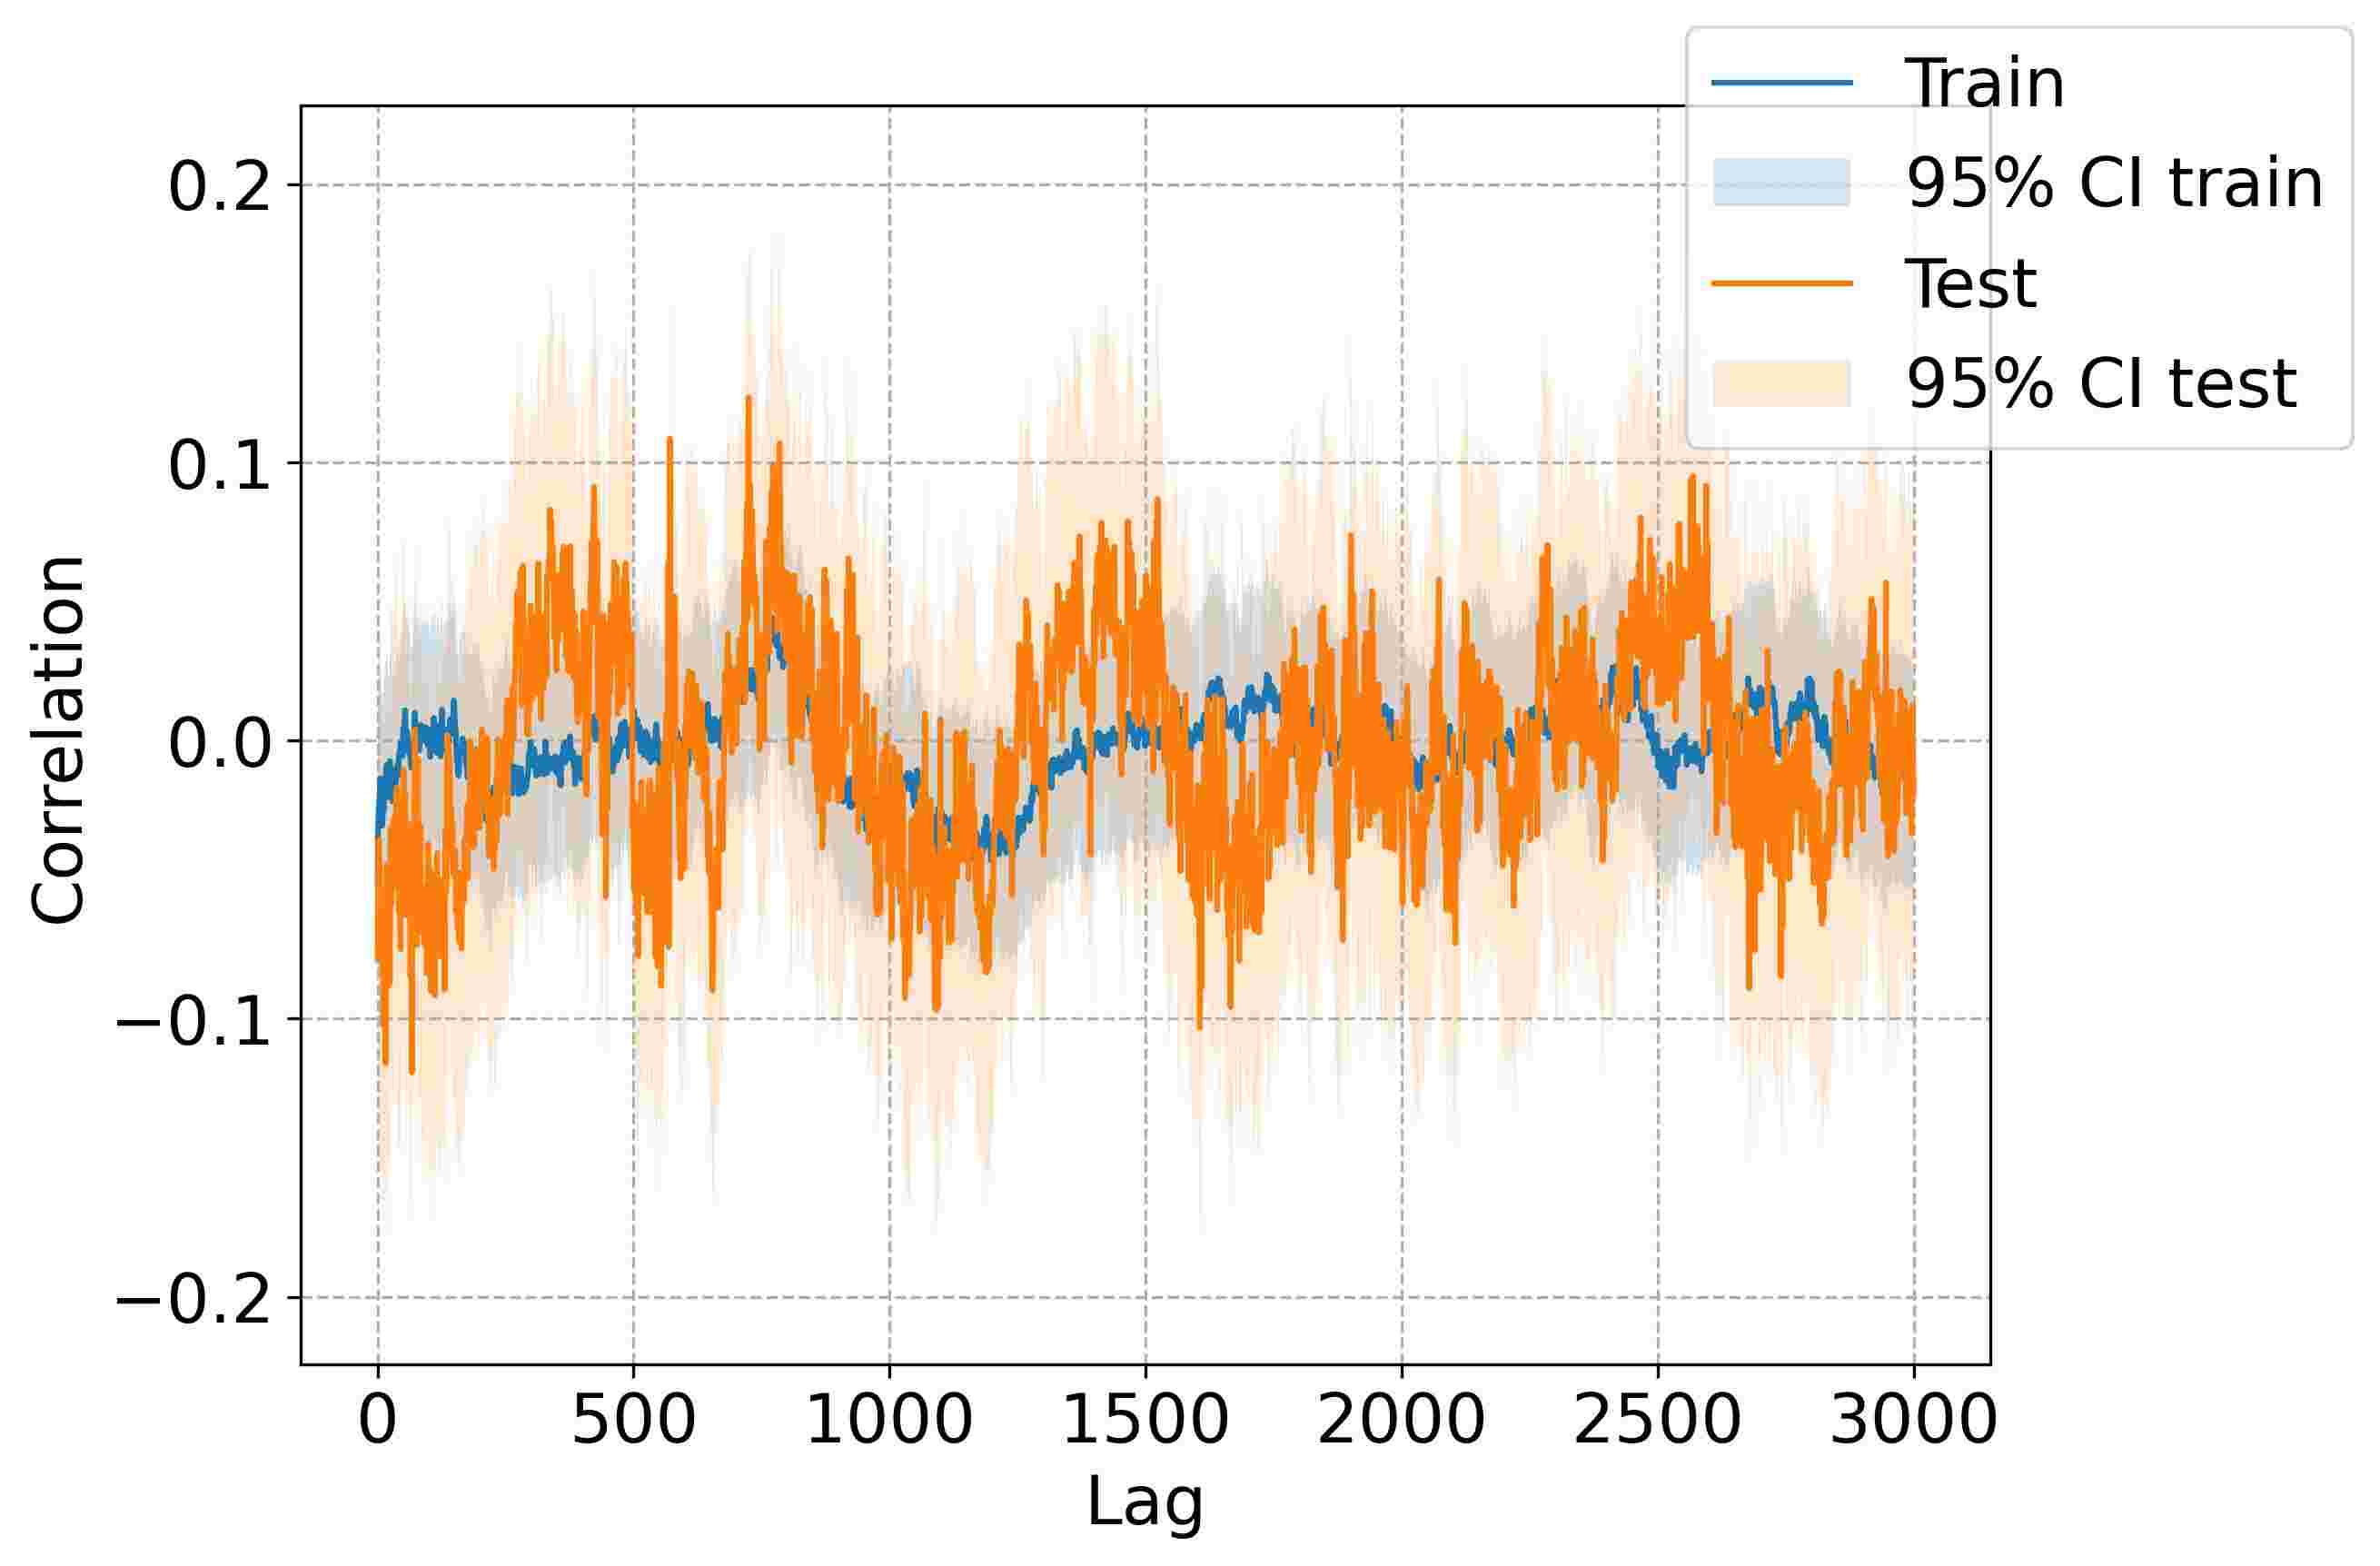
\includegraphics[width=0.3\linewidth]{STXE24MO_R1_Correlation.jpg}}
    \caption{Correlation between the ATM implied volatility and the daily returns as a function of the lag both on the train and the test sets. The 95\% confidence intervals are derived from the Fisher transformation. }
\label{fig:corr_structure_r1}
\end{figure}




\section{Study of the calibrated parameters}

We conclude this empirical study by analyzing the calibrated parameters of the PDV model. In order to obtain comparable model parameters between time-to-maturities, we retain a single triplet $(C_{R_1},C_{\Sigma},\lambda)$ for all time-to-maturities. This triplet is selected as follows. For each time-to-maturity, we compute the average $R^2$ score over the 10 folds of each triplet and then, we average these scores over all time-to-maturities. Finally, for each triplet $(C_{R_1},C_{\Sigma},\lambda)$, we average the obtained score with the one of the triplets $(C_{R_1}',C_{\Sigma}',\lambda')$ such that $C'_{\Sigma}=C_{\Sigma}$ and either $C_{R_1}'$ is the closest value above or below $C_{R_1}$ in the grid $\{5,10,25,50,100,250,500,1000,\dots,2500,3000\}$ or $\lambda'$ is the closest value above or below $\lambda$ in the grid $\{10^{-6},10^{-5},\dots,10^{-1}\}$. For example, the score of the triplet $(50,500,10^{-3})$ is averaged with the one of the triplets $(25,500,10^{-3})$, $(100,500,10^{-3})$, $(50,500,10^{-4})$ and $(50,500,10^{-2})$. The triplet that is chosen for all time-to-maturities is the one achieving the higher score through this procedure. This procedure aims at selecting a triplet whose performance is not too sensitive to a modification of $C_{R_1}$ or $\lambda$ and is introduced because we observed that if we consider only the average score over all time-to-maturities, the performance of the obtained triplet was very sensitive to these two hyperparameters (unlike most triplets as underlined earlier) and was quite bad on the test set. This instability is probably due to the small size of the train set which is divided in 10 folds in the blocked cross-validation. With this procedure, we obtain $(C_{R_1},C_{\Sigma},\lambda)=(250,1000,10^{-3})$ for the S\&P 500 and $(C_{R_1},C_{\Sigma},\lambda)=(10,1000,10^{-3})$ for the Euro Stoxx 50. In Figure \ref{fig:r2_cross_valid}, we show the $R^2$ scores obtained on the train and the test sets with these hyperparameters. We notice overall that the obtained $R^2$ scores are very close to those presented in Figure \ref{fig:r2_cutoff_1000} where $(C_{R_1},C_{\Sigma},\lambda)=(1000,1000,0)$. This is due to the fact that the cut-off lag $C_{\Sigma}$ of the volatility did not change between the two figures and, as described in Appendix \ref{sec:influence_cutoff}, the two other hyperparameters $C_{R_1}$ and $\lambda$ have a small influence. \\

\begin{figure}[h]
    \centering
    \subfigure[S\&P 500]{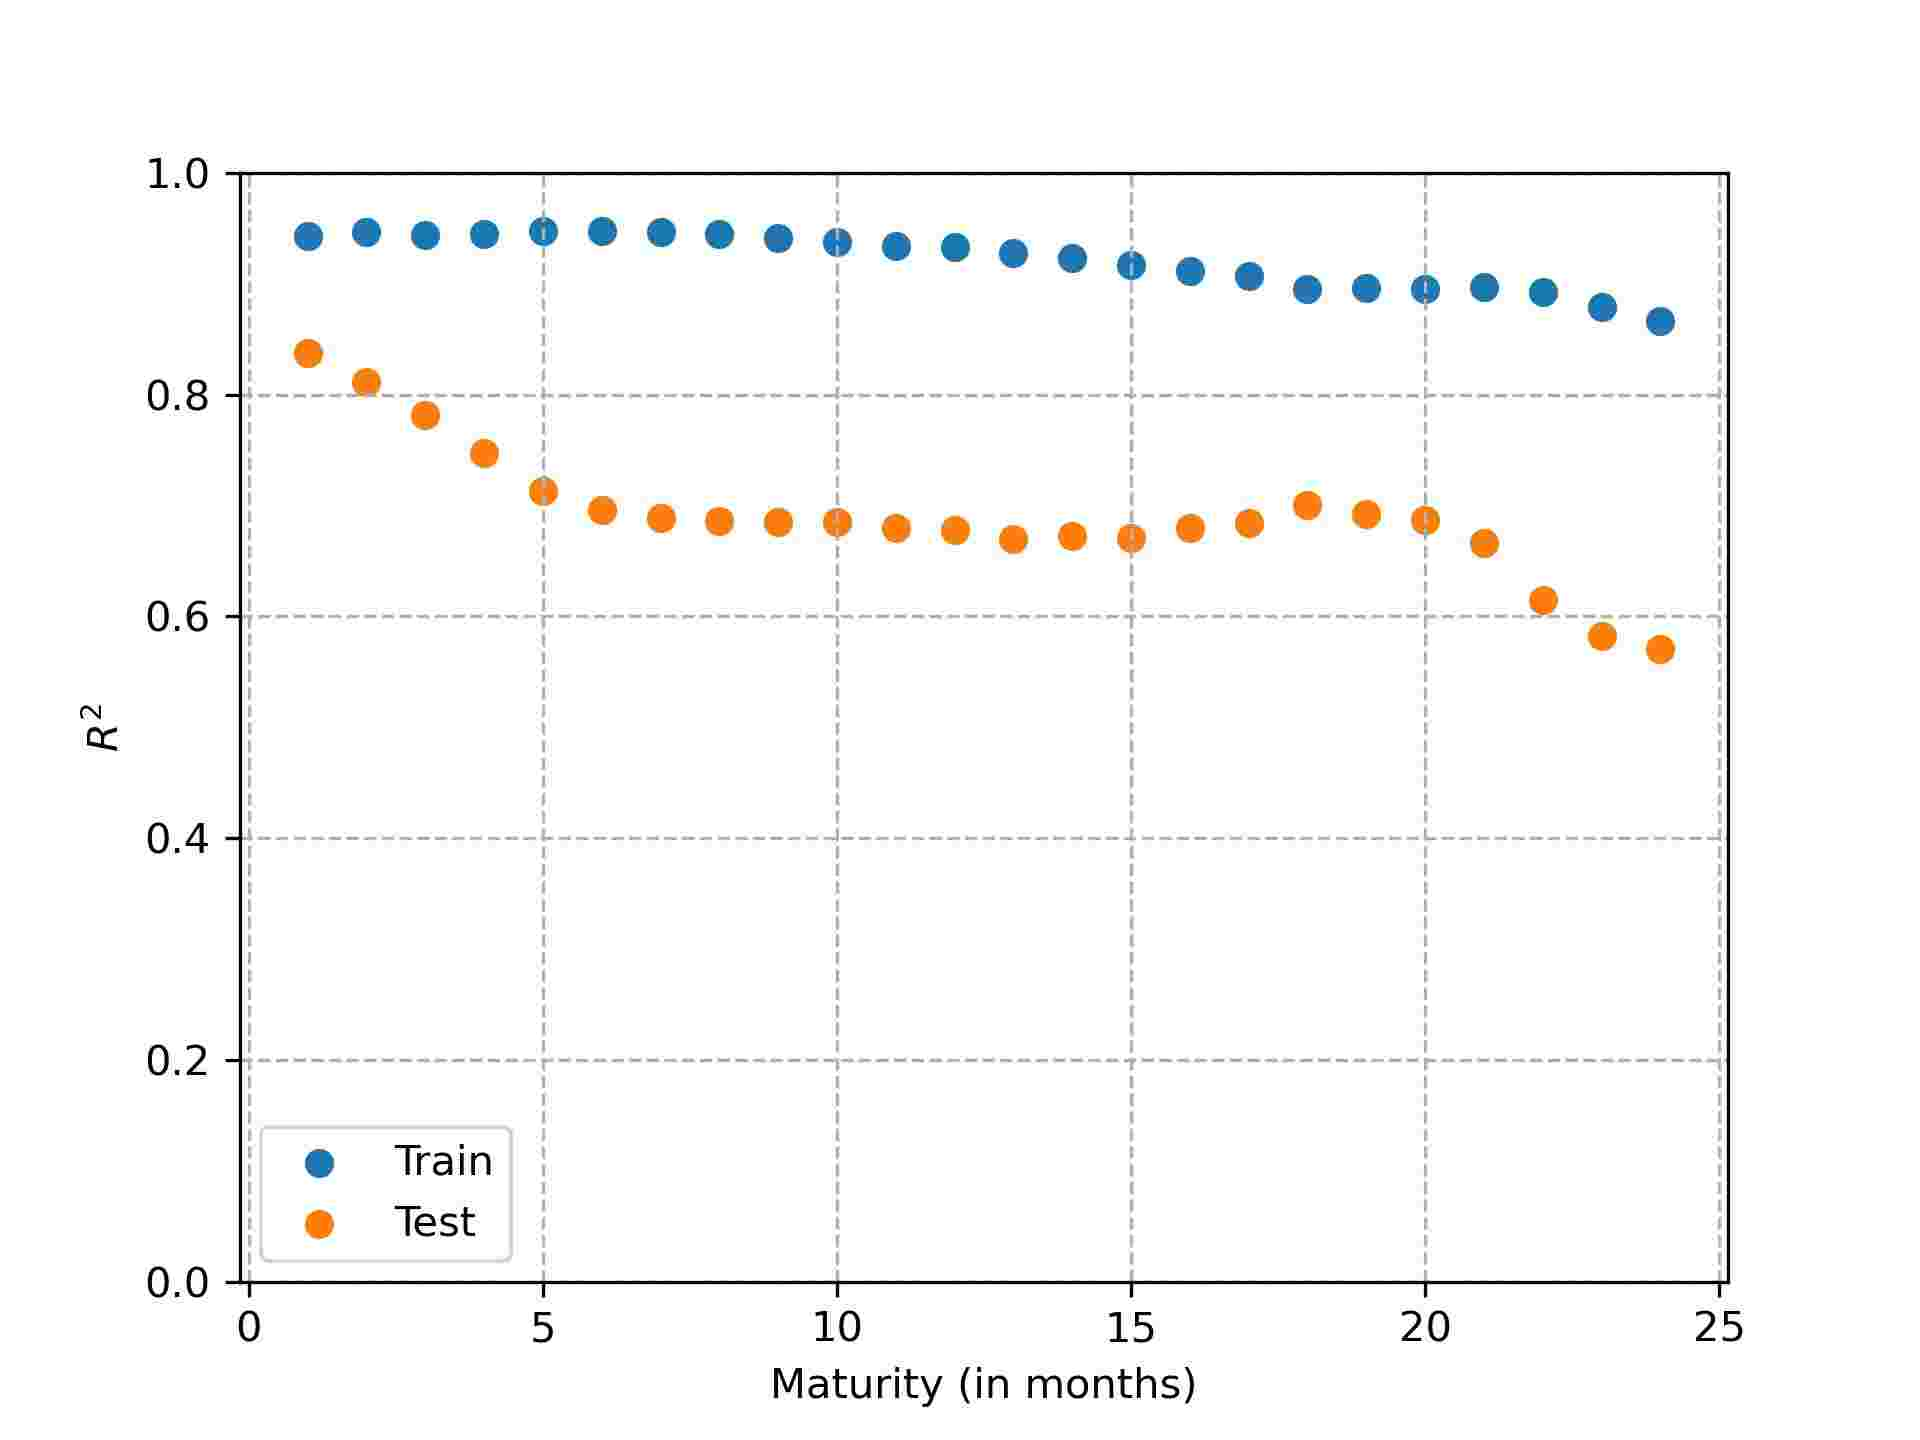
\includegraphics[width=0.45\linewidth]{SPX_Optimal_Scores_Best_HyperParams.jpg}}
    \subfigure[Euro Stoxx 50]{ 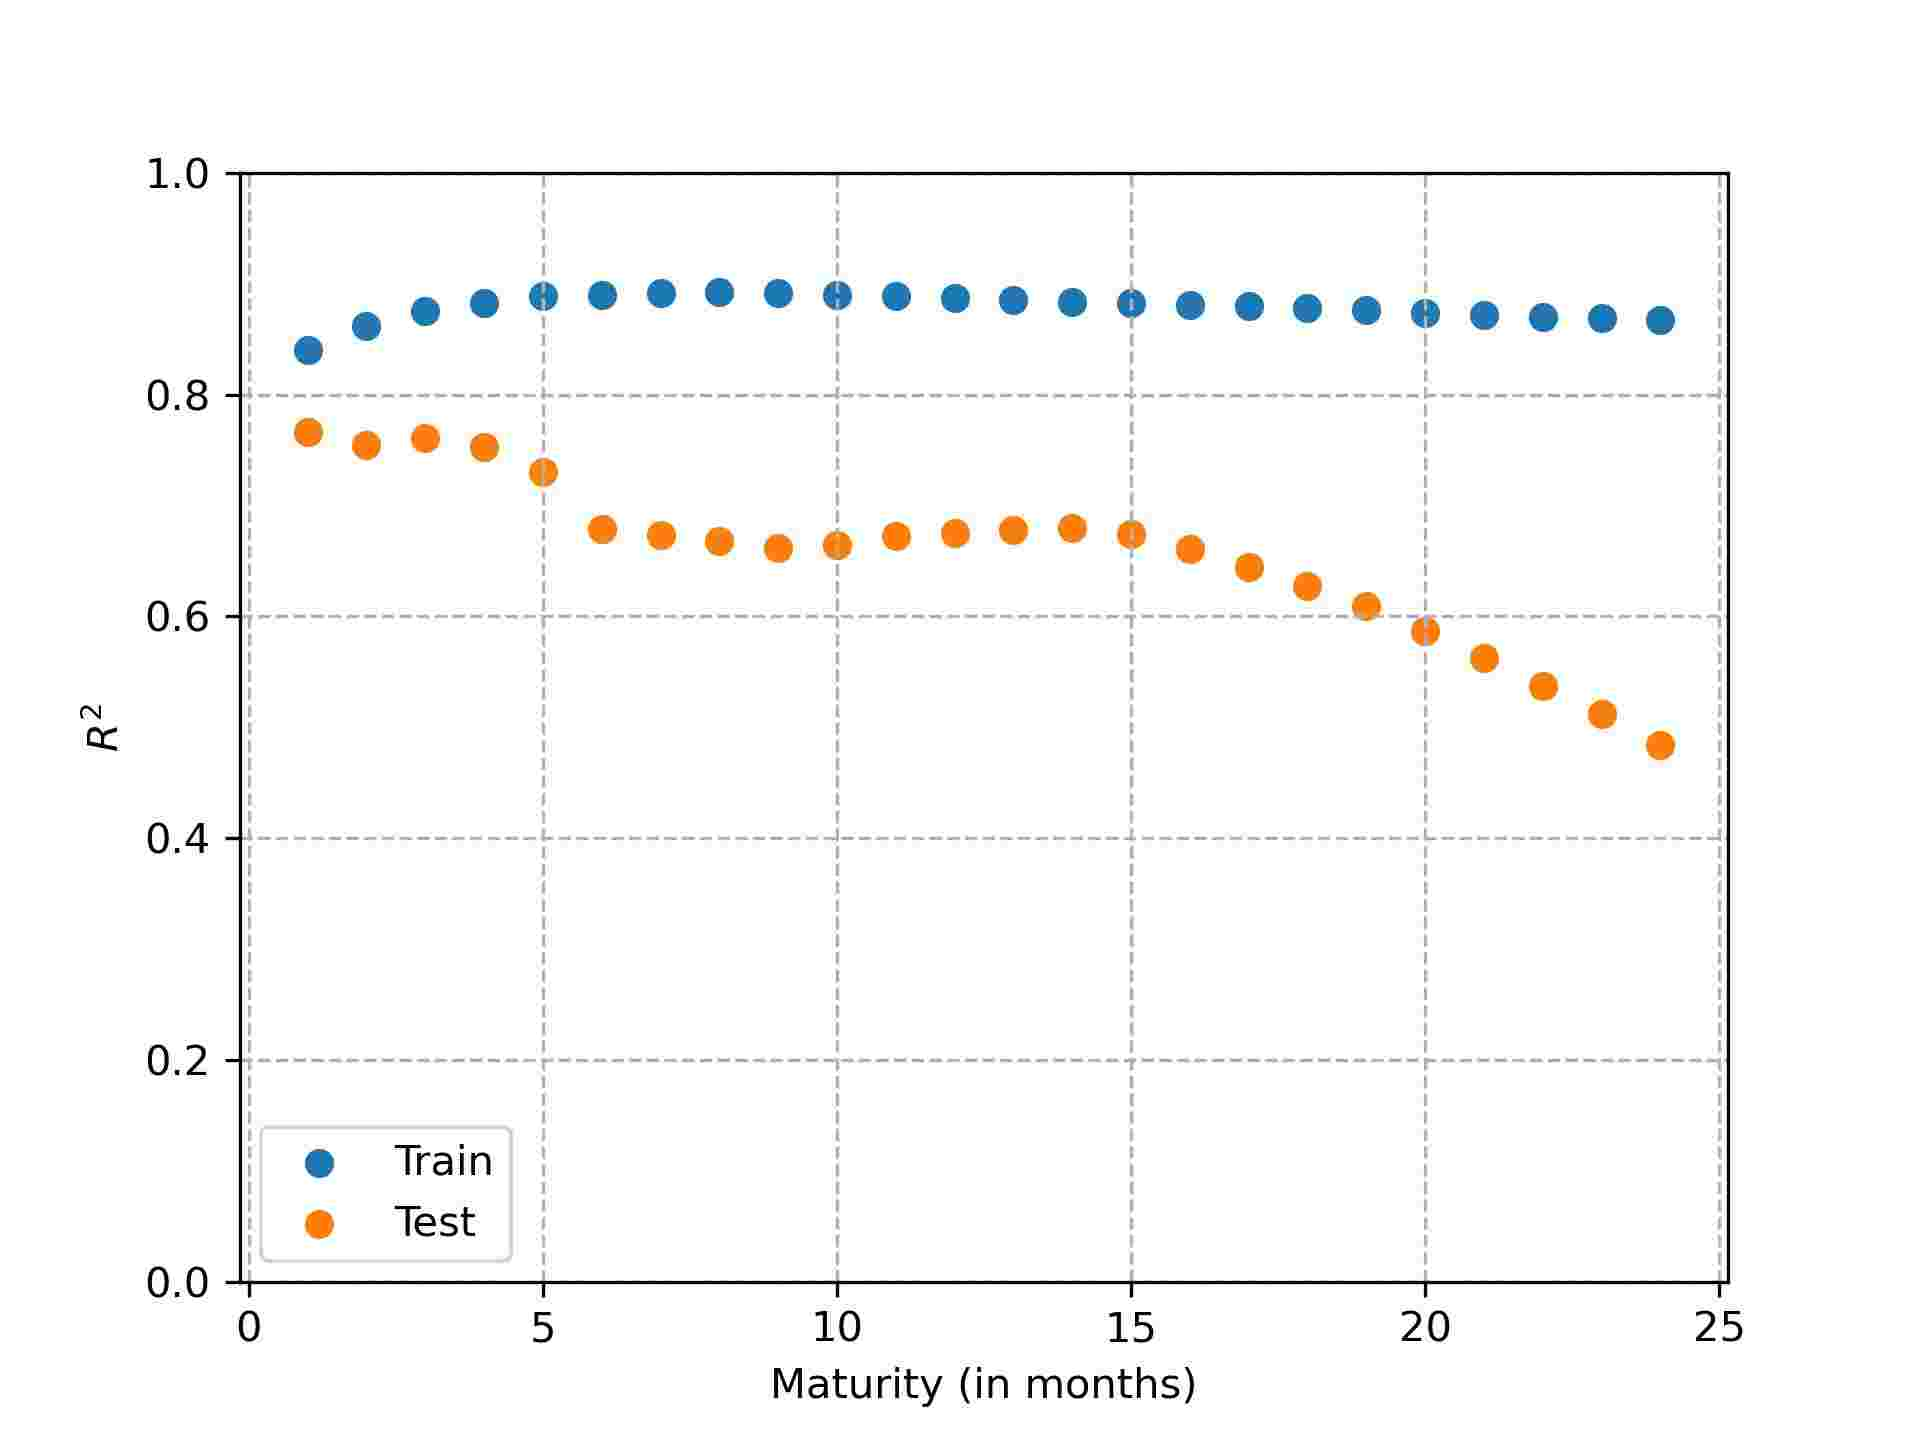
\includegraphics[width=0.45\linewidth]{STXE_Optimal_Scores_Best_HyperParams.jpg}}
    \caption{$R^2$ scores on the train and the test sets as a function of the ATM implied volatility time-to-maturity. The hyperparameters for the S\&P 500 are $(C_{R_1,C_{\Sigma},\lambda)=(250,1000,10^{-3})}$ and those of the Euro Stoxx 50 are $(C_{R_1},C_{\Sigma},\lambda)=(10,1000,10^{-3})$. }
\label{fig:r2_cross_valid}
\end{figure} 
In Figures \ref{fig:pdv_params_tspl} and \ref{fig:pdv_params_lin_reg}, we plot the evolution of the calibrated parameters associated to the $R^2$ scores presented in Figure \ref{fig:r2_cross_valid} as a function of the time-to-maturity. Regarding the TSPL kernels parameters ($\alpha_1$, $\delta_1$, $\alpha_2$, $\delta_2$), we observe overall a decreasing trend except for $\delta_2$ for which there is no clear trend. This decreasing trend for $\alpha_1$ and $\alpha_2$ indicates that far away past returns explain more and more the ATM implied volatility movements as the time-to-maturity increases. Note that, for the largest time-to-maturities, we obtain values of $\alpha$ that become even lower than 1 (except for $\alpha_1$ for the S\&P 500) which is the critical value below which the integral of the TSPL kernel diverges in continuous time. The decreasing behavior of $\delta_1$ indicates that, as $\alpha_1$ decreases, it still matters to keep a large weight for the more recent returns. Let us now end the study with the analysis of the parameters $\beta_0$, $\beta_1$ and $\beta_2$. First, we notice that we have $\beta_1<0$ and $\beta_2>0$ without imposing any constraint on these parameters. Therefore, a positive (resp. negative) trend in the underlying asset price tends to be followed by a decrease (resp. increase) of the implied volatility (which is consistent with the negative correlation observed by \cite{cont2002dynamics}) while the increase (resp. decrease) of the underlying asset volatility (measured by the squared returns) tends to be followed by an increase (resp. decrease) of the implied volatility. Moreover, the three parameters for the small time-to-maturities are of the same order of magnitude as to those calibrated by \cite{guyon2022volatility}. Regarding the evolution of $\beta_0$, we obtain an overall increase with the time-to-maturity which reflects the fact that, in average, the level of ATM implied volatility increases with the time-to-maturity. The parameter $\beta_1$, which can be interpreted as the influence of the trend feature on the implied volatility, has opposite evolutions for the S\&P 500 and the Euro Stoxx 50 (it is essentially decreasing for the former and increasing for the latter). Thus, it is difficult to draw any conclusion. Finally, the parameter $\beta_2$, which can be interpreted as the influence of the volatility feature on the implied volatility, is mainly decreasing with the time-to-maturity, so it seems that the implied volatility for long time-to-maturities becomes less reactive to the volatility of the underlying index. \\
\begin{figure}[ht]
    \centering
    \subfigure[$\alpha_1$ (S\&P 500)]{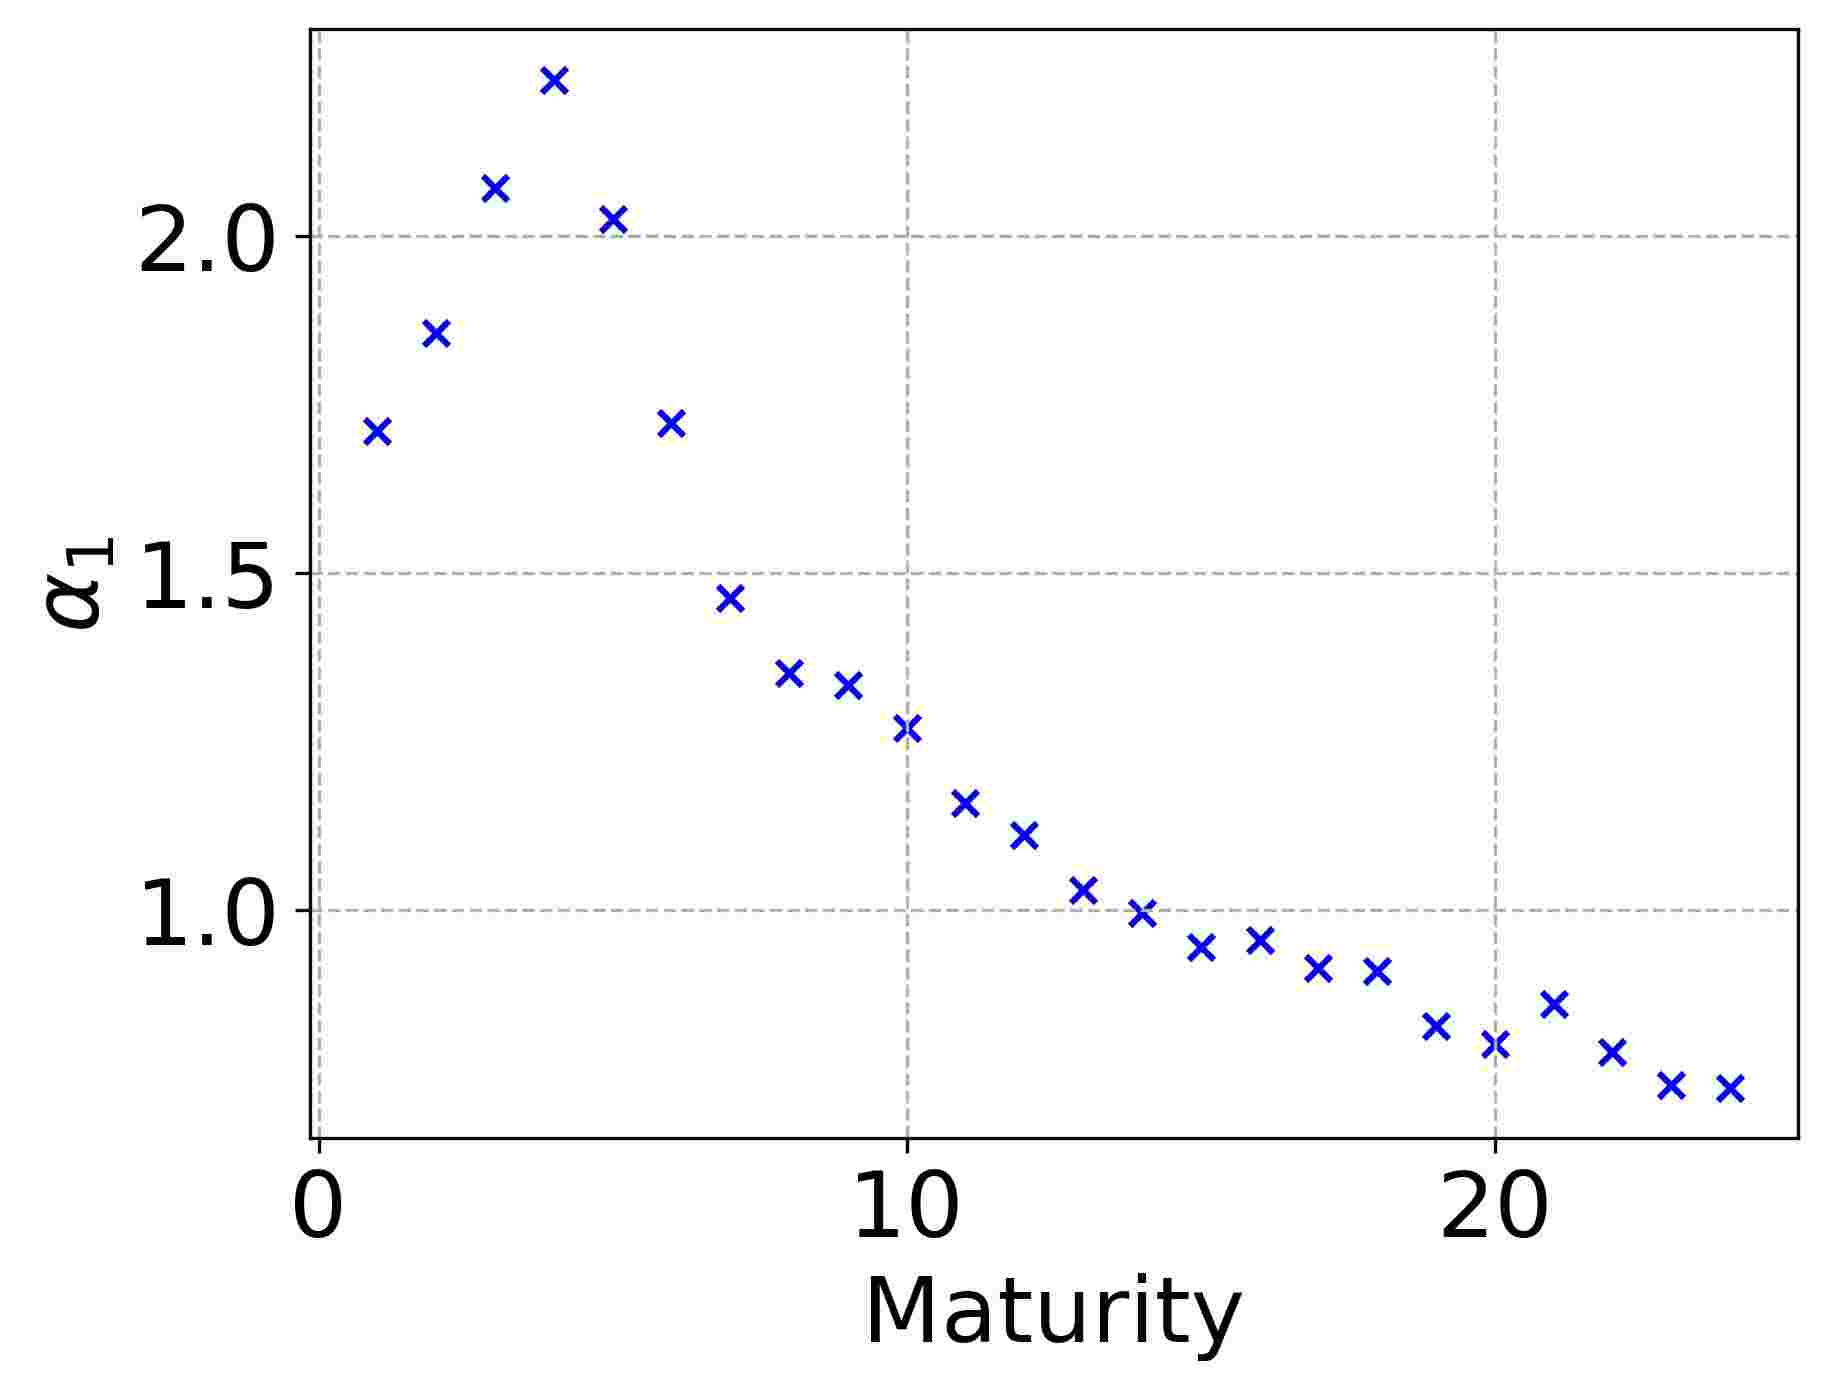
\includegraphics[width=0.23\linewidth]{SPX_alpha_1.jpg}    }
    \subfigure[$\delta_1$ (S\&P 500)]{ 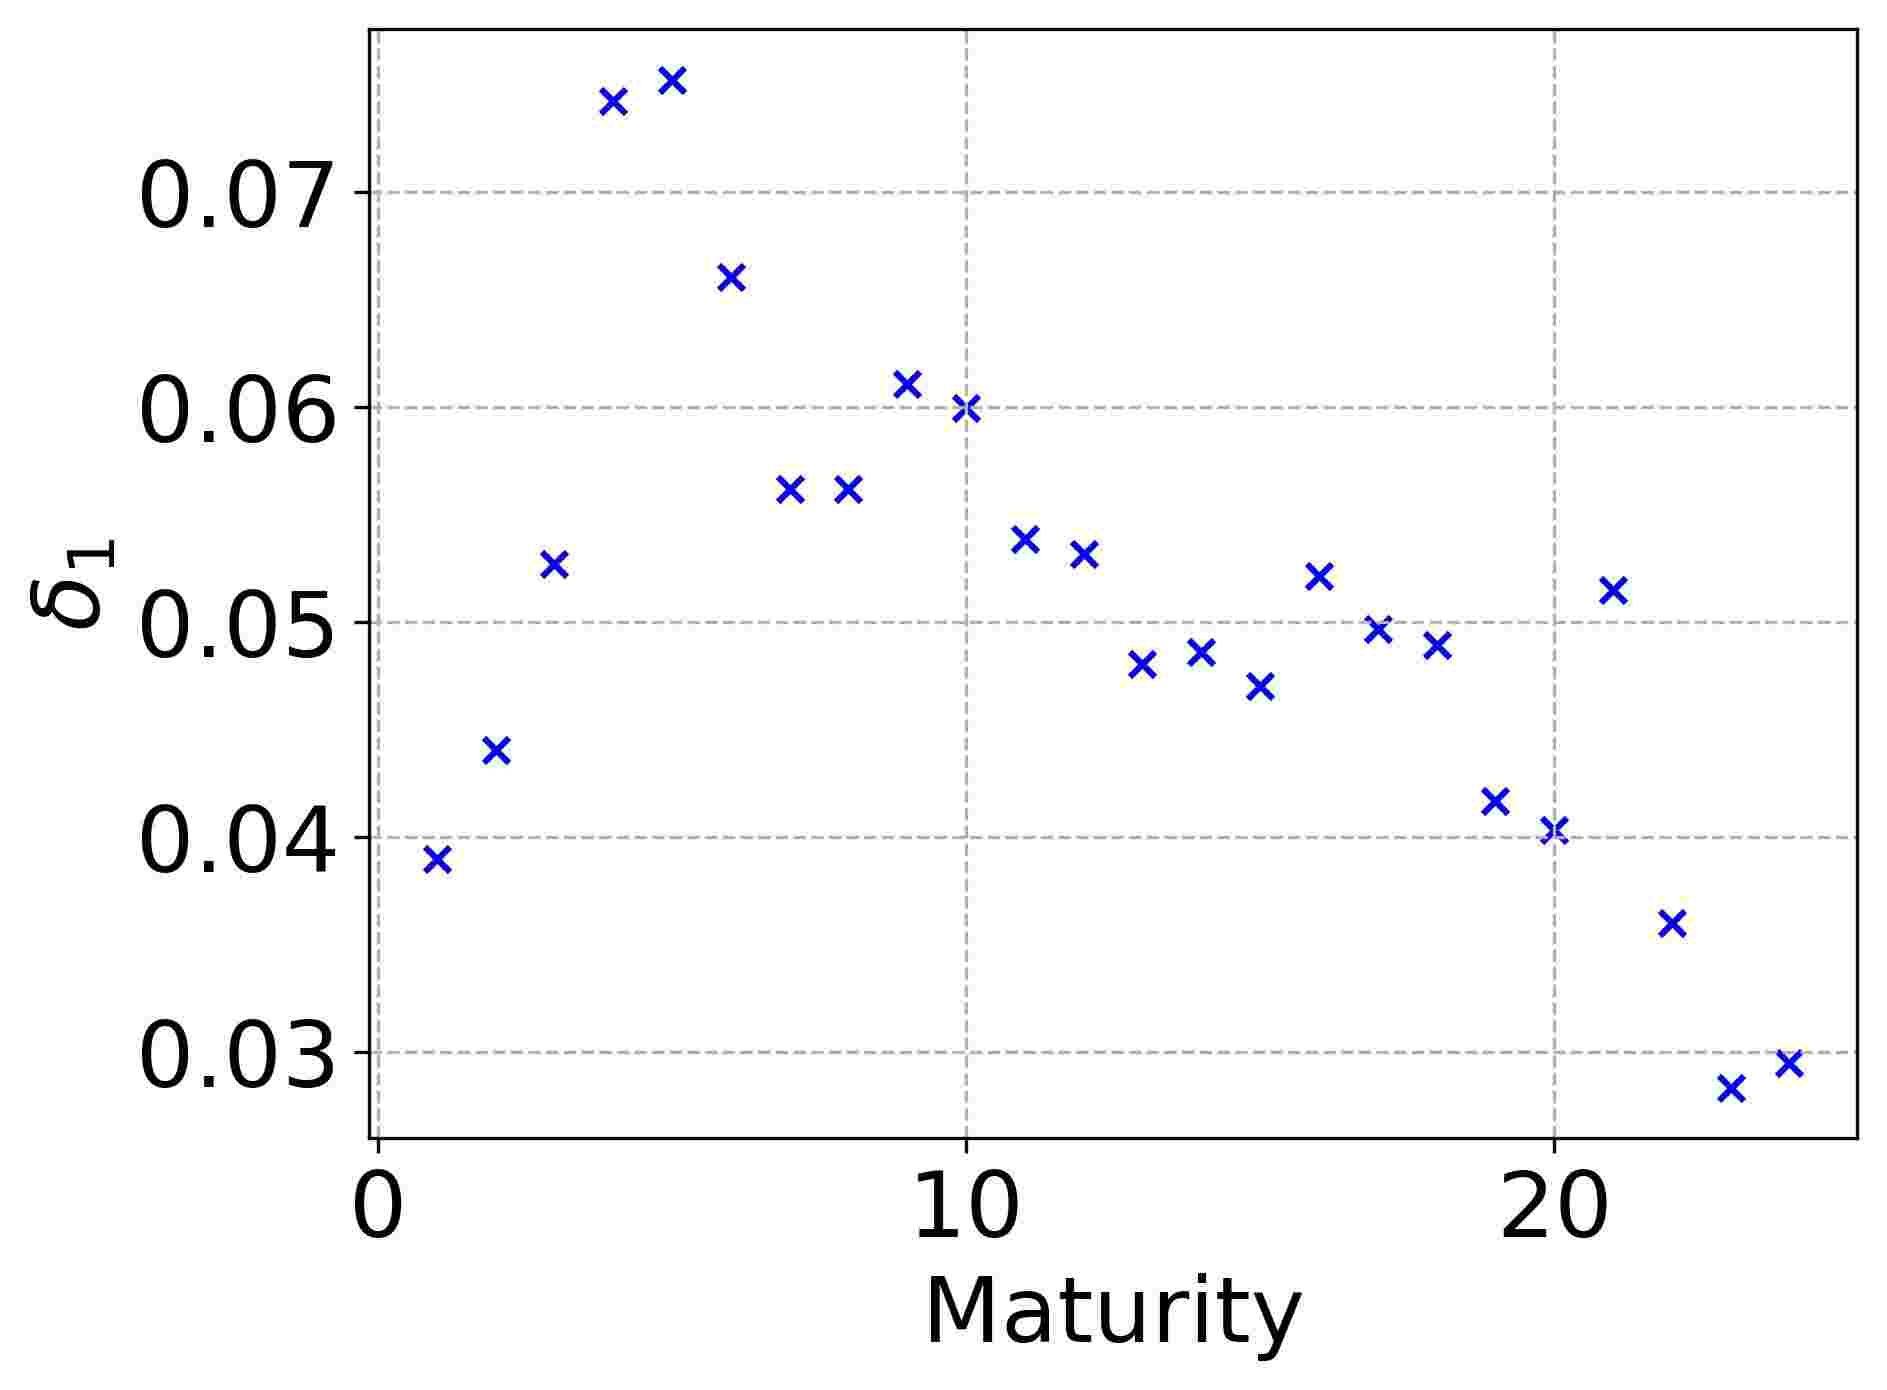
\includegraphics[width=0.23\linewidth]{SPX_delta_1.jpg}}
    \subfigure[$\alpha_2$ (S\&P 500)]{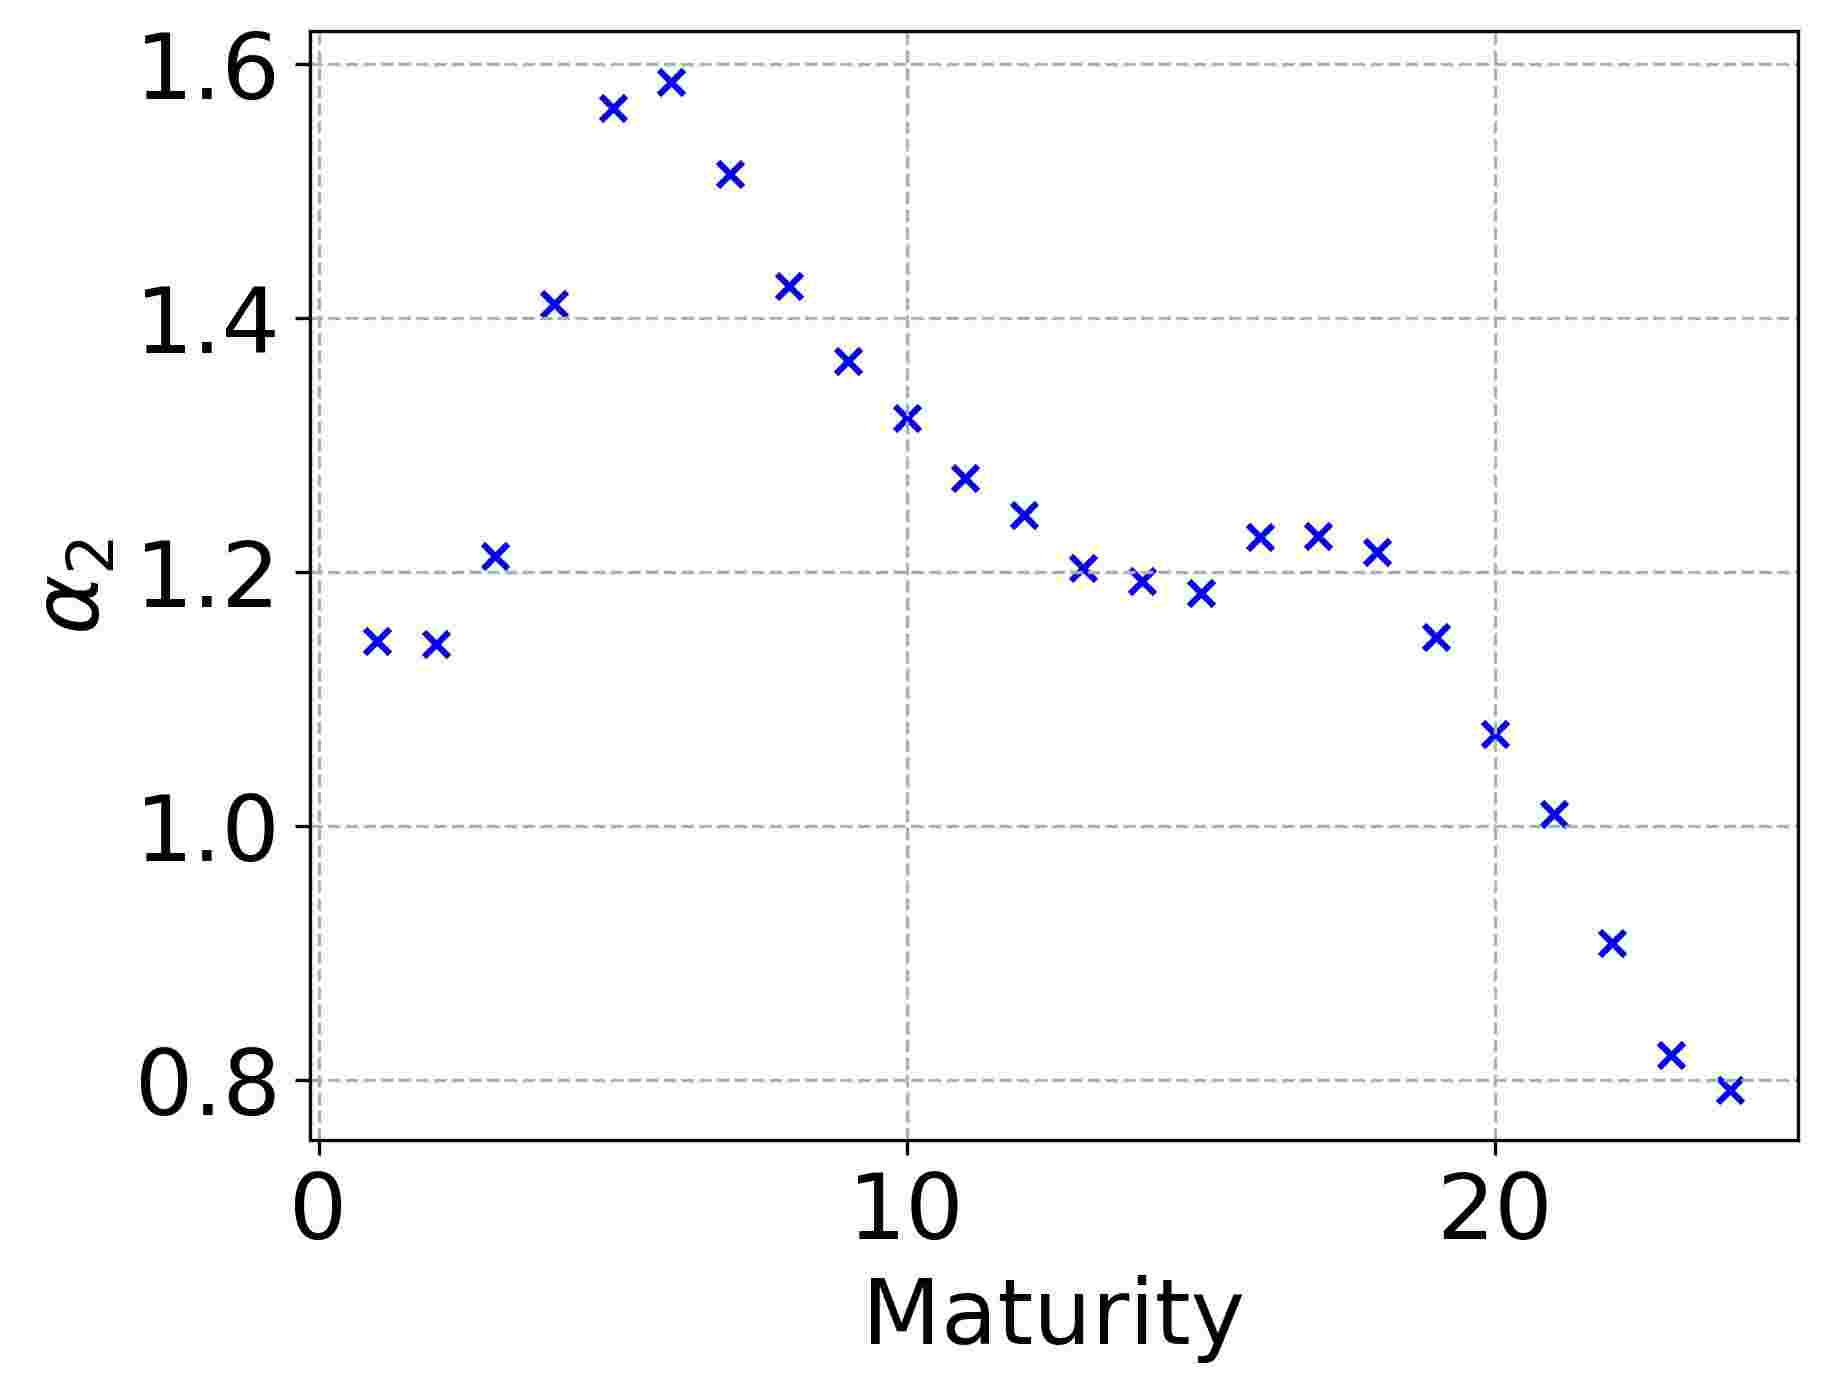
\includegraphics[width=0.23\linewidth]{SPX_alpha_2.jpg}}
    \subfigure[$\delta_2$ (S\&P 500)]{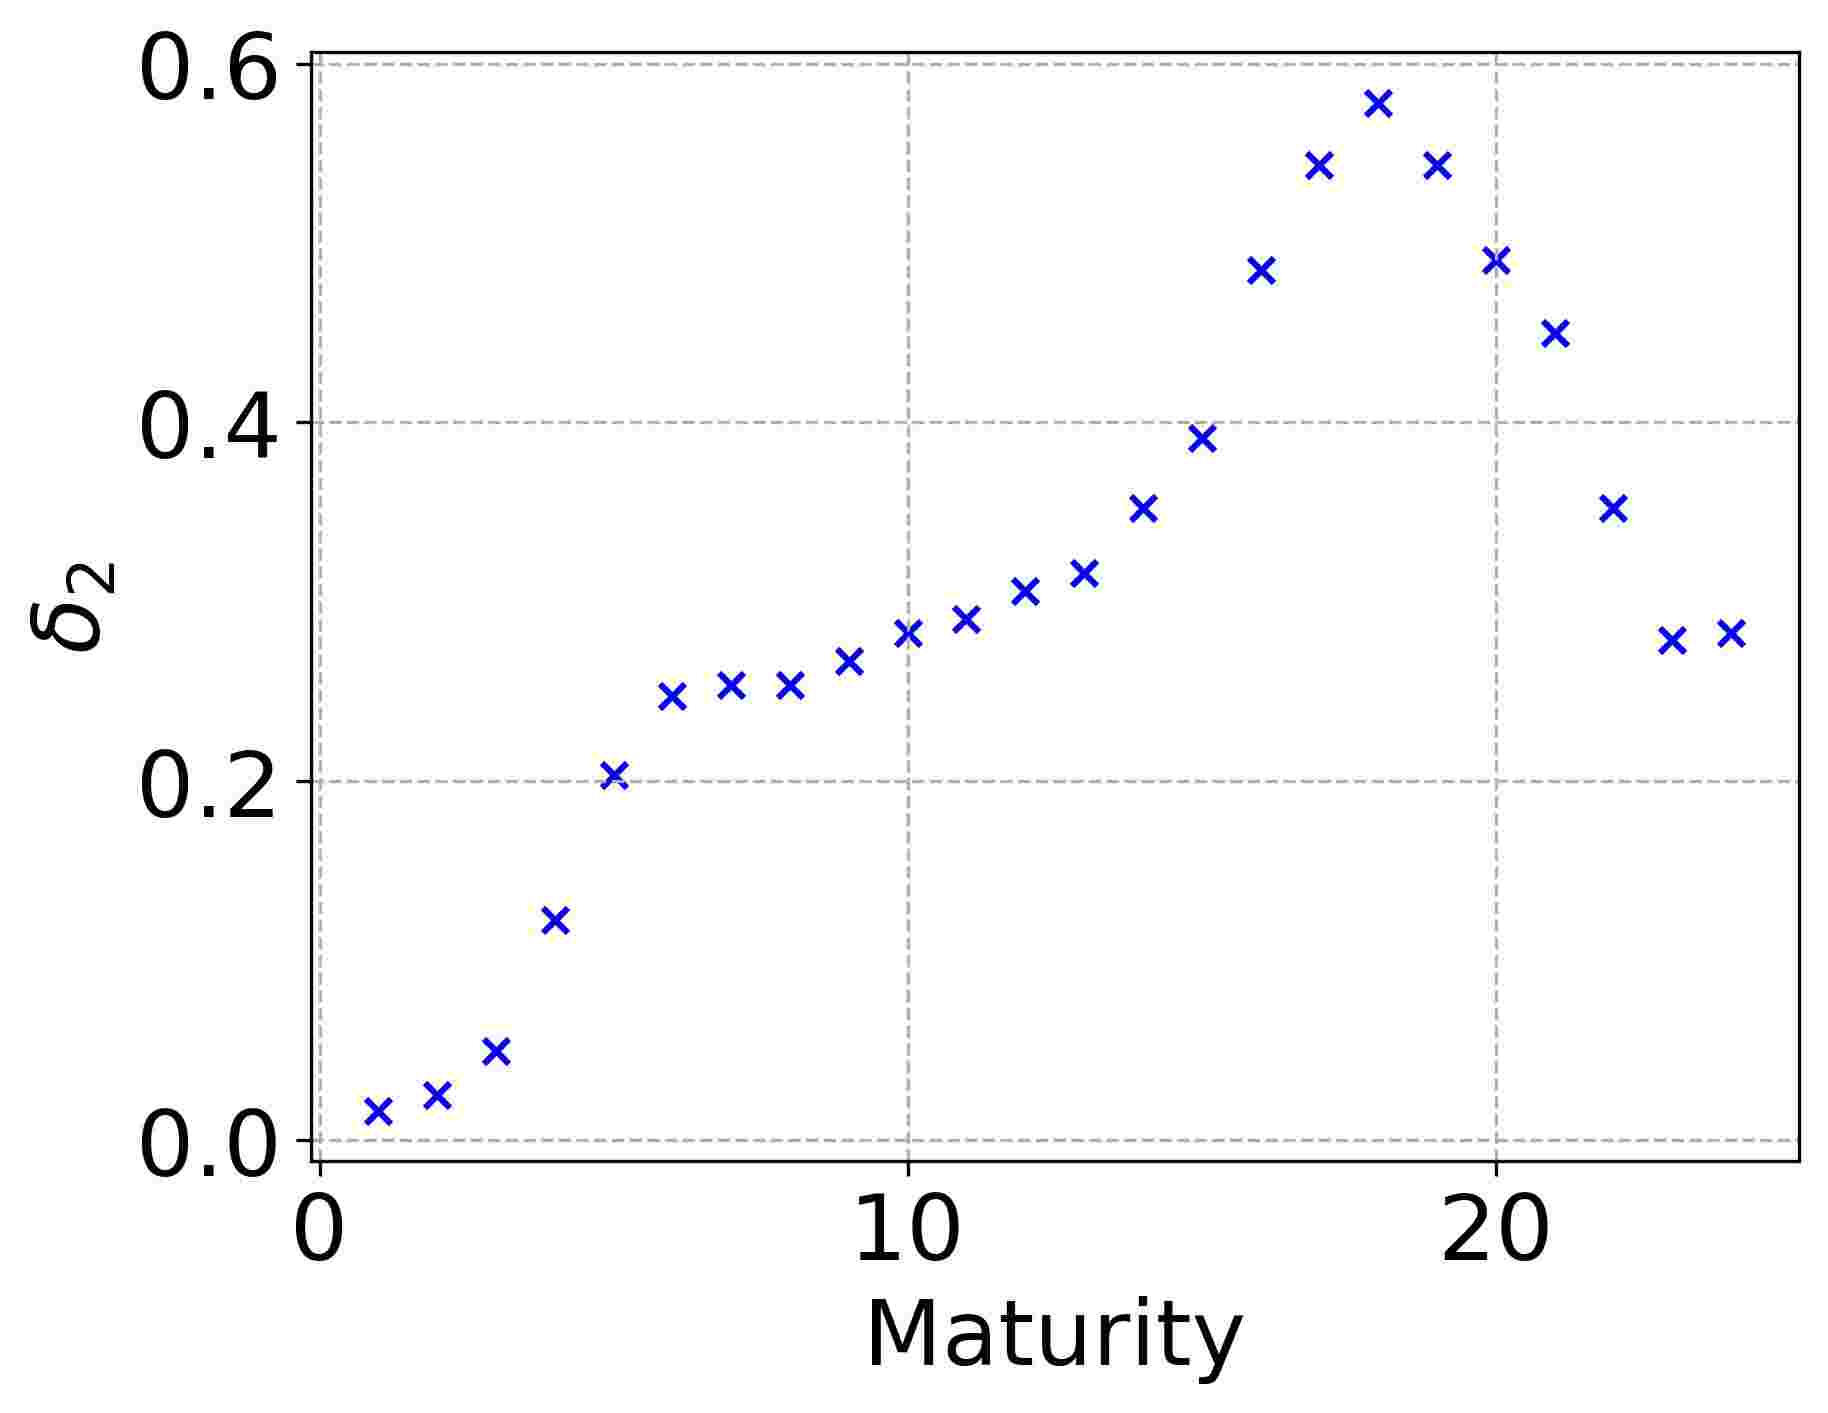
\includegraphics[width=0.23\linewidth]{SPX_delta_2.jpg}}
    \subfigure[$\alpha_1$ (Euro Stoxx 50)]{ 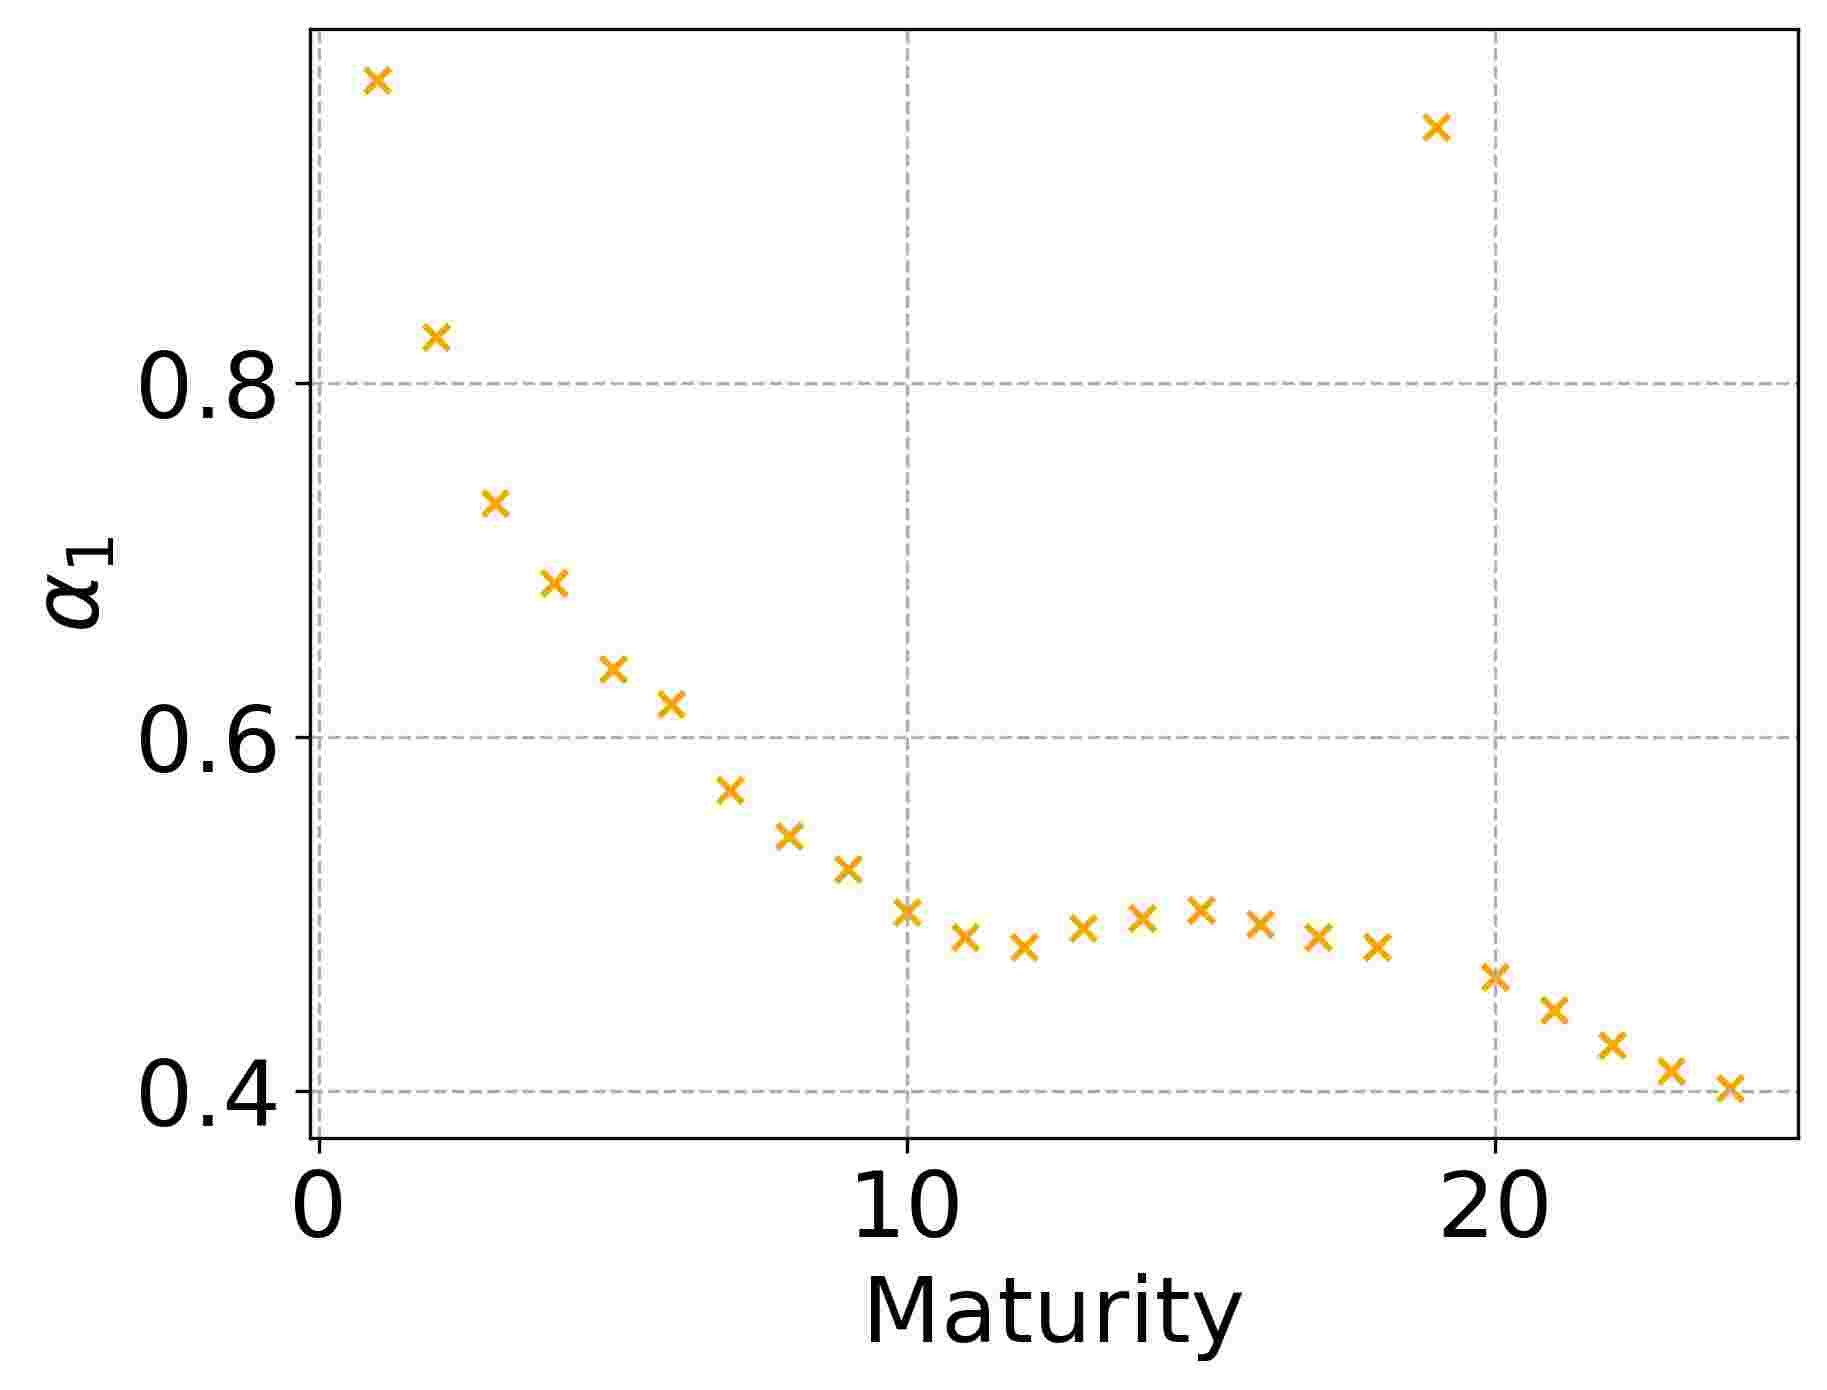
\includegraphics[width=0.23\linewidth]{STXE_alpha_1.jpg}}
    \subfigure[$\delta_1$ (Euro Stoxx 50)]{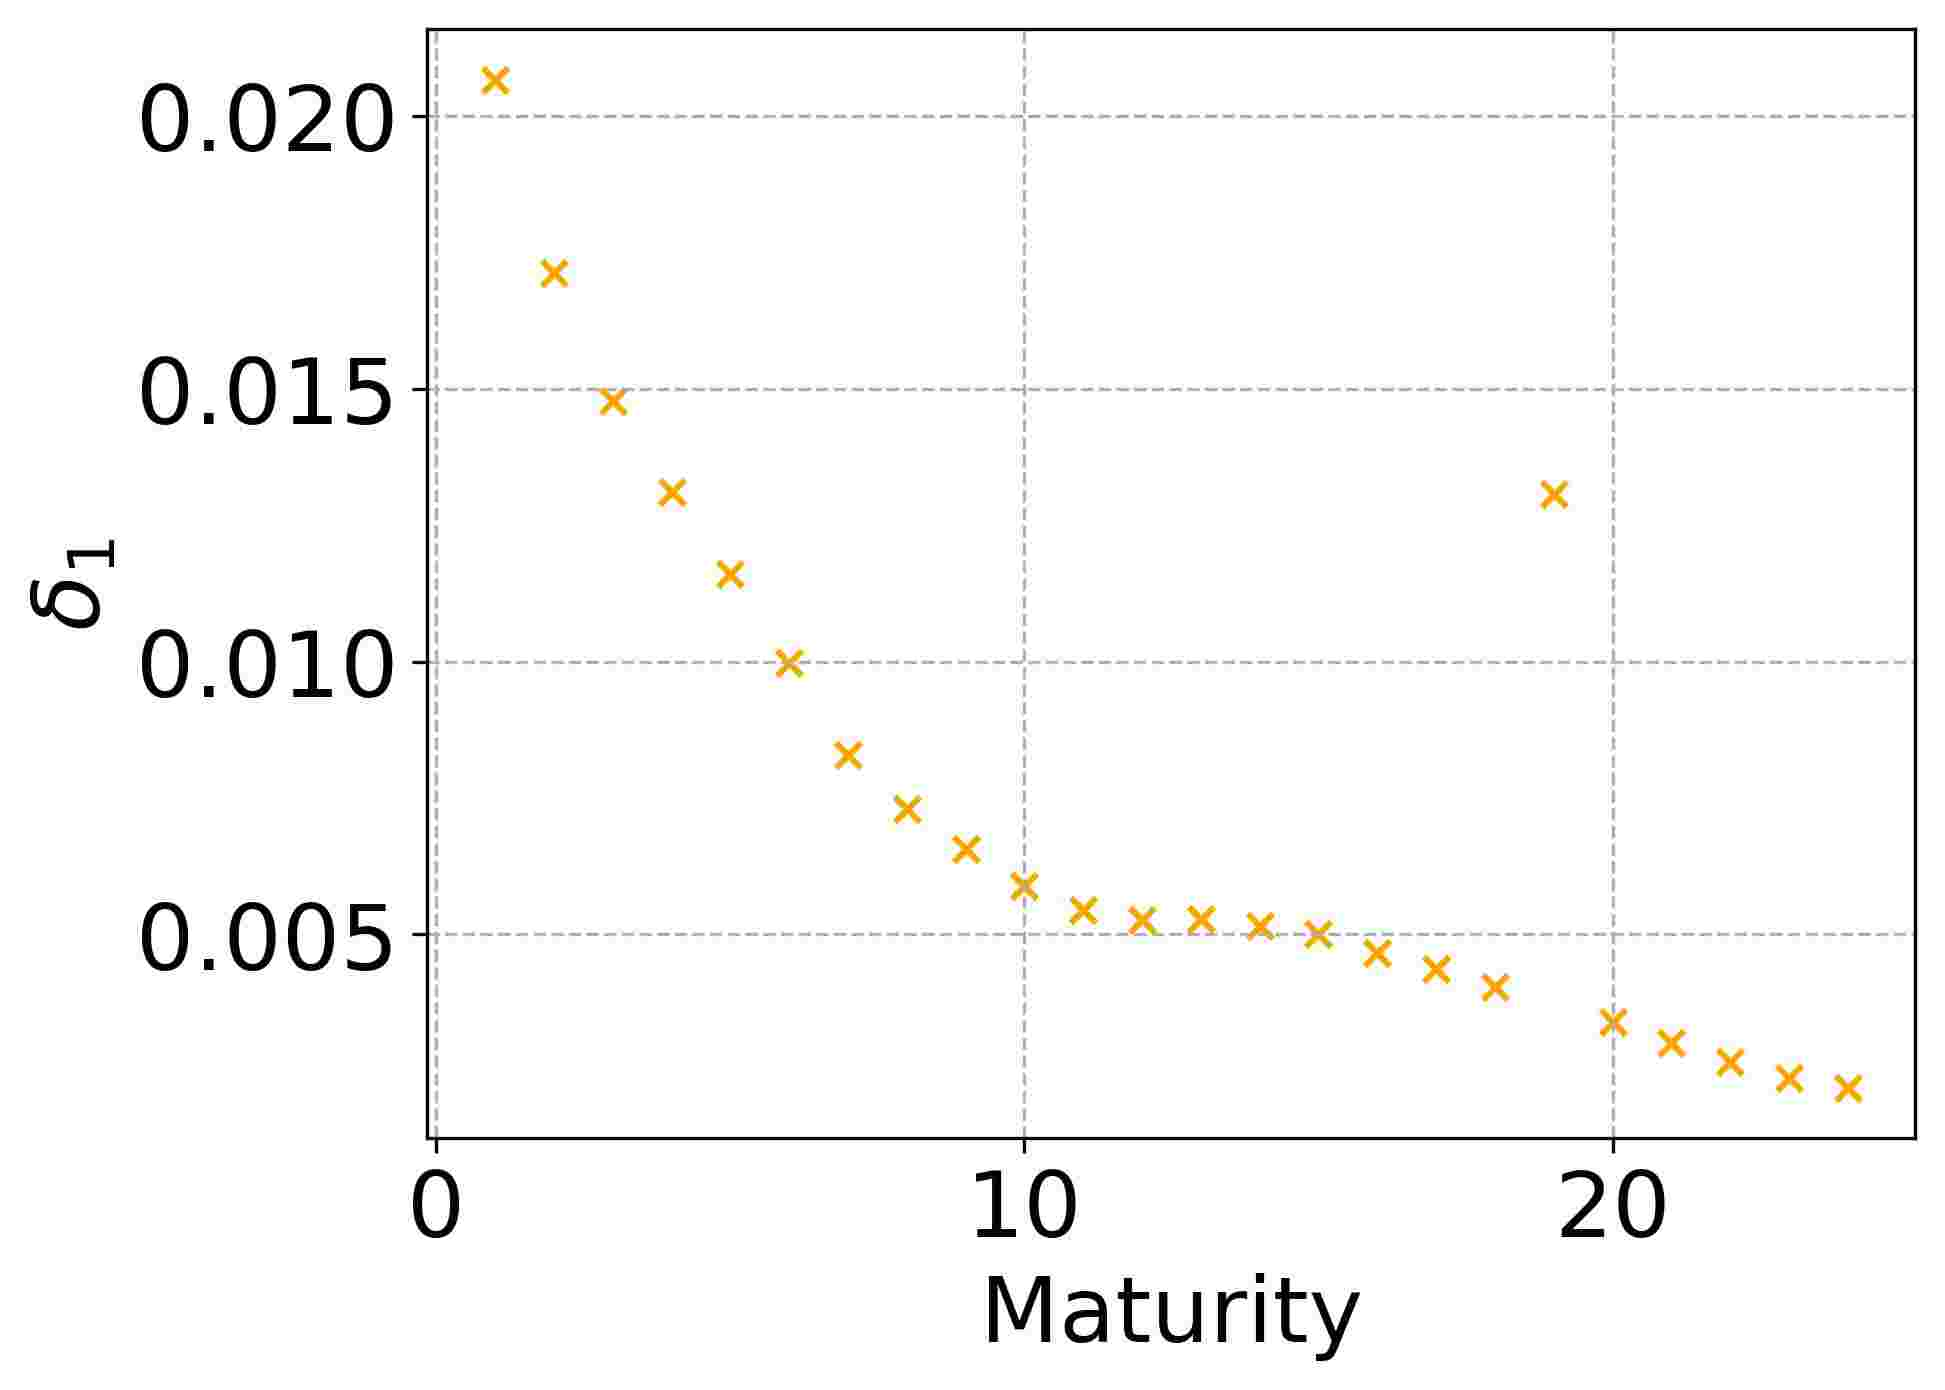
\includegraphics[width=0.23\linewidth]{STXE_delta_1.jpg}}
    \subfigure[$\alpha_2$ (Euro Stoxx 50)]{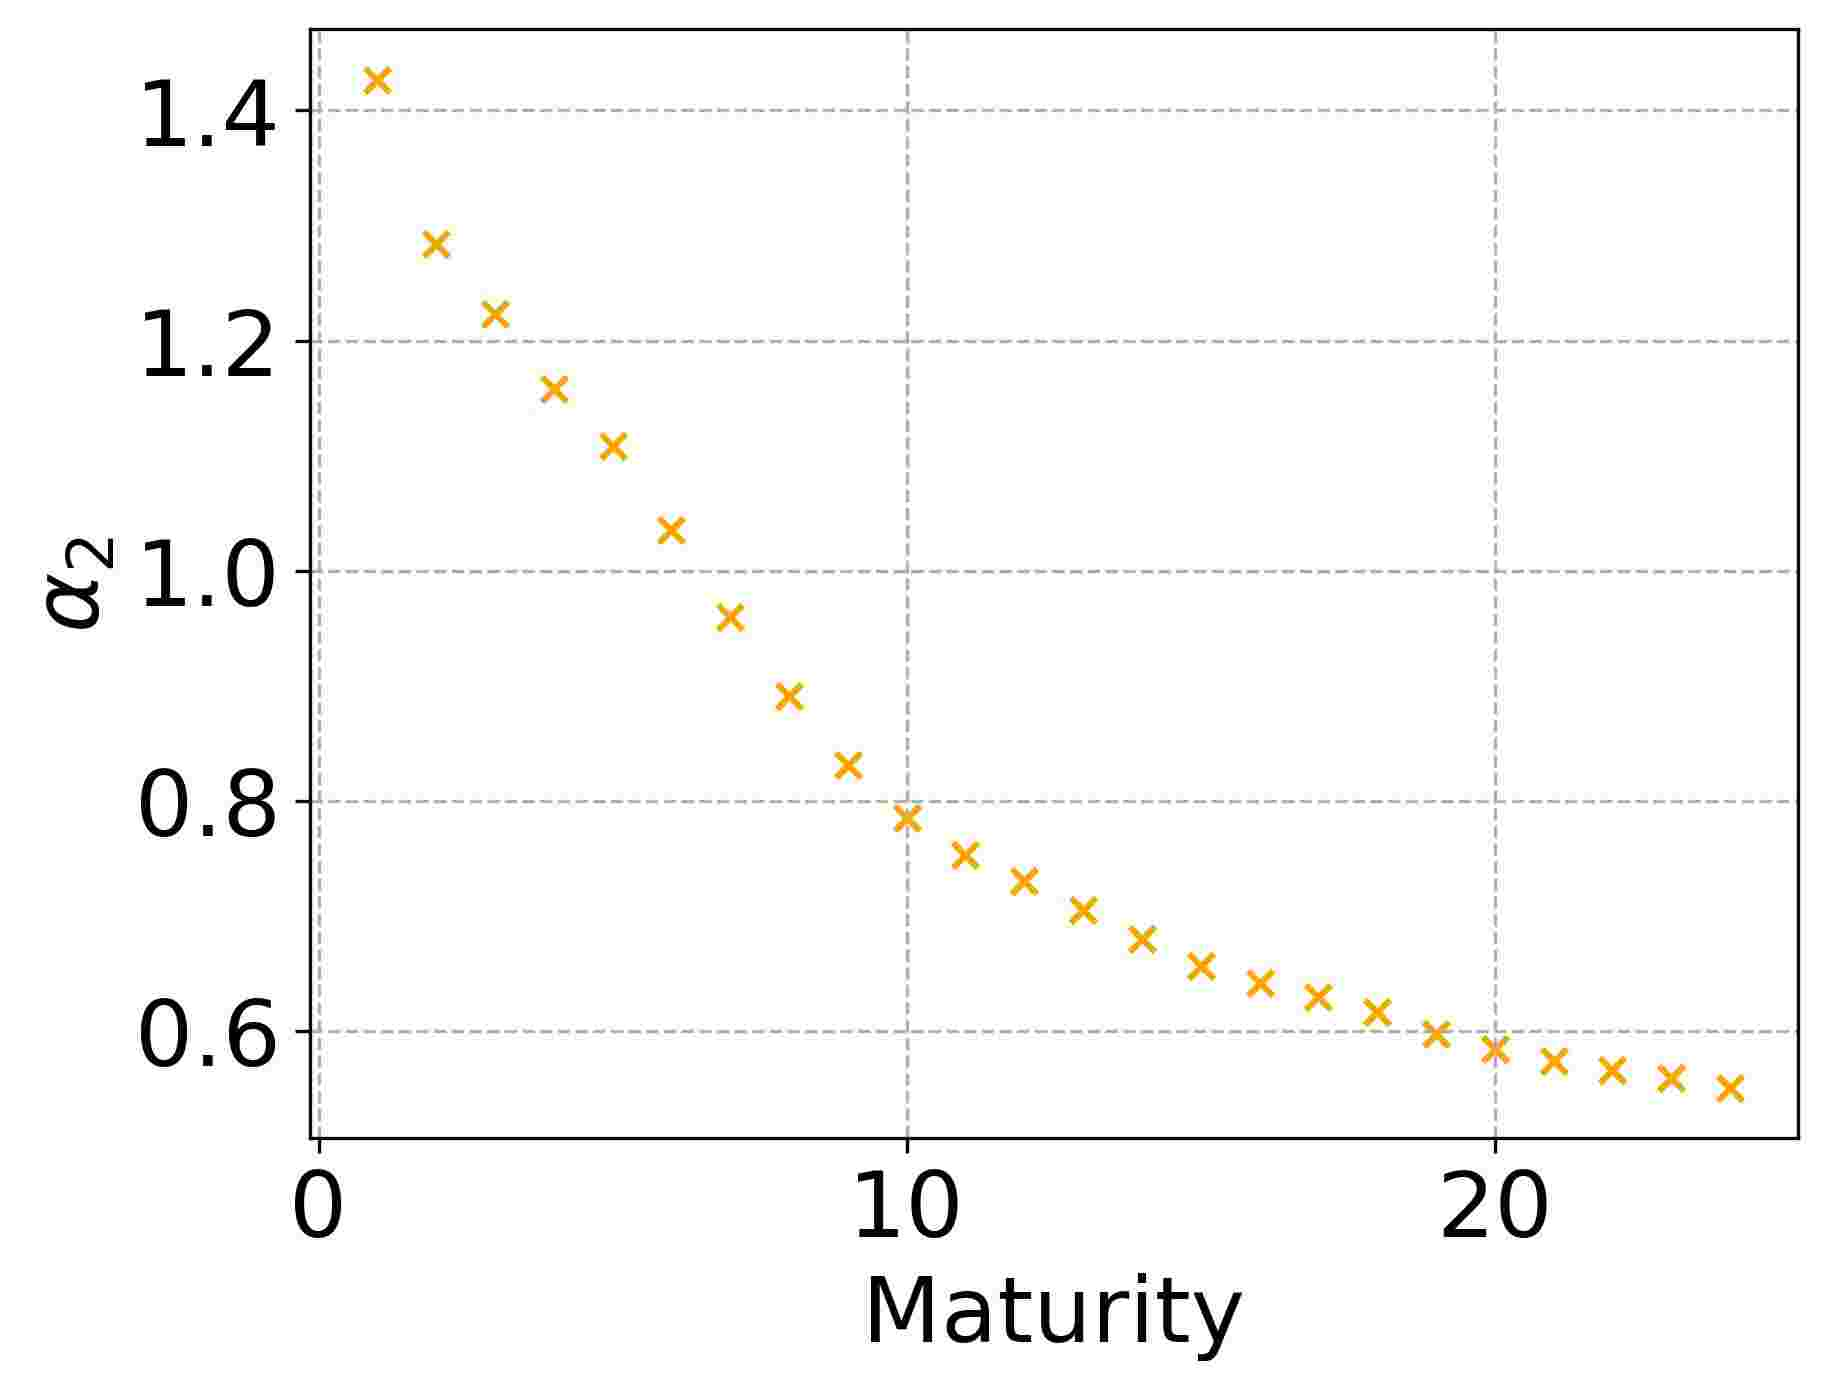
\includegraphics[width=0.23\linewidth]{STXE_alpha_2.jpg}}
    \subfigure[$\delta_2$ (Euro Stoxx 50)]{ 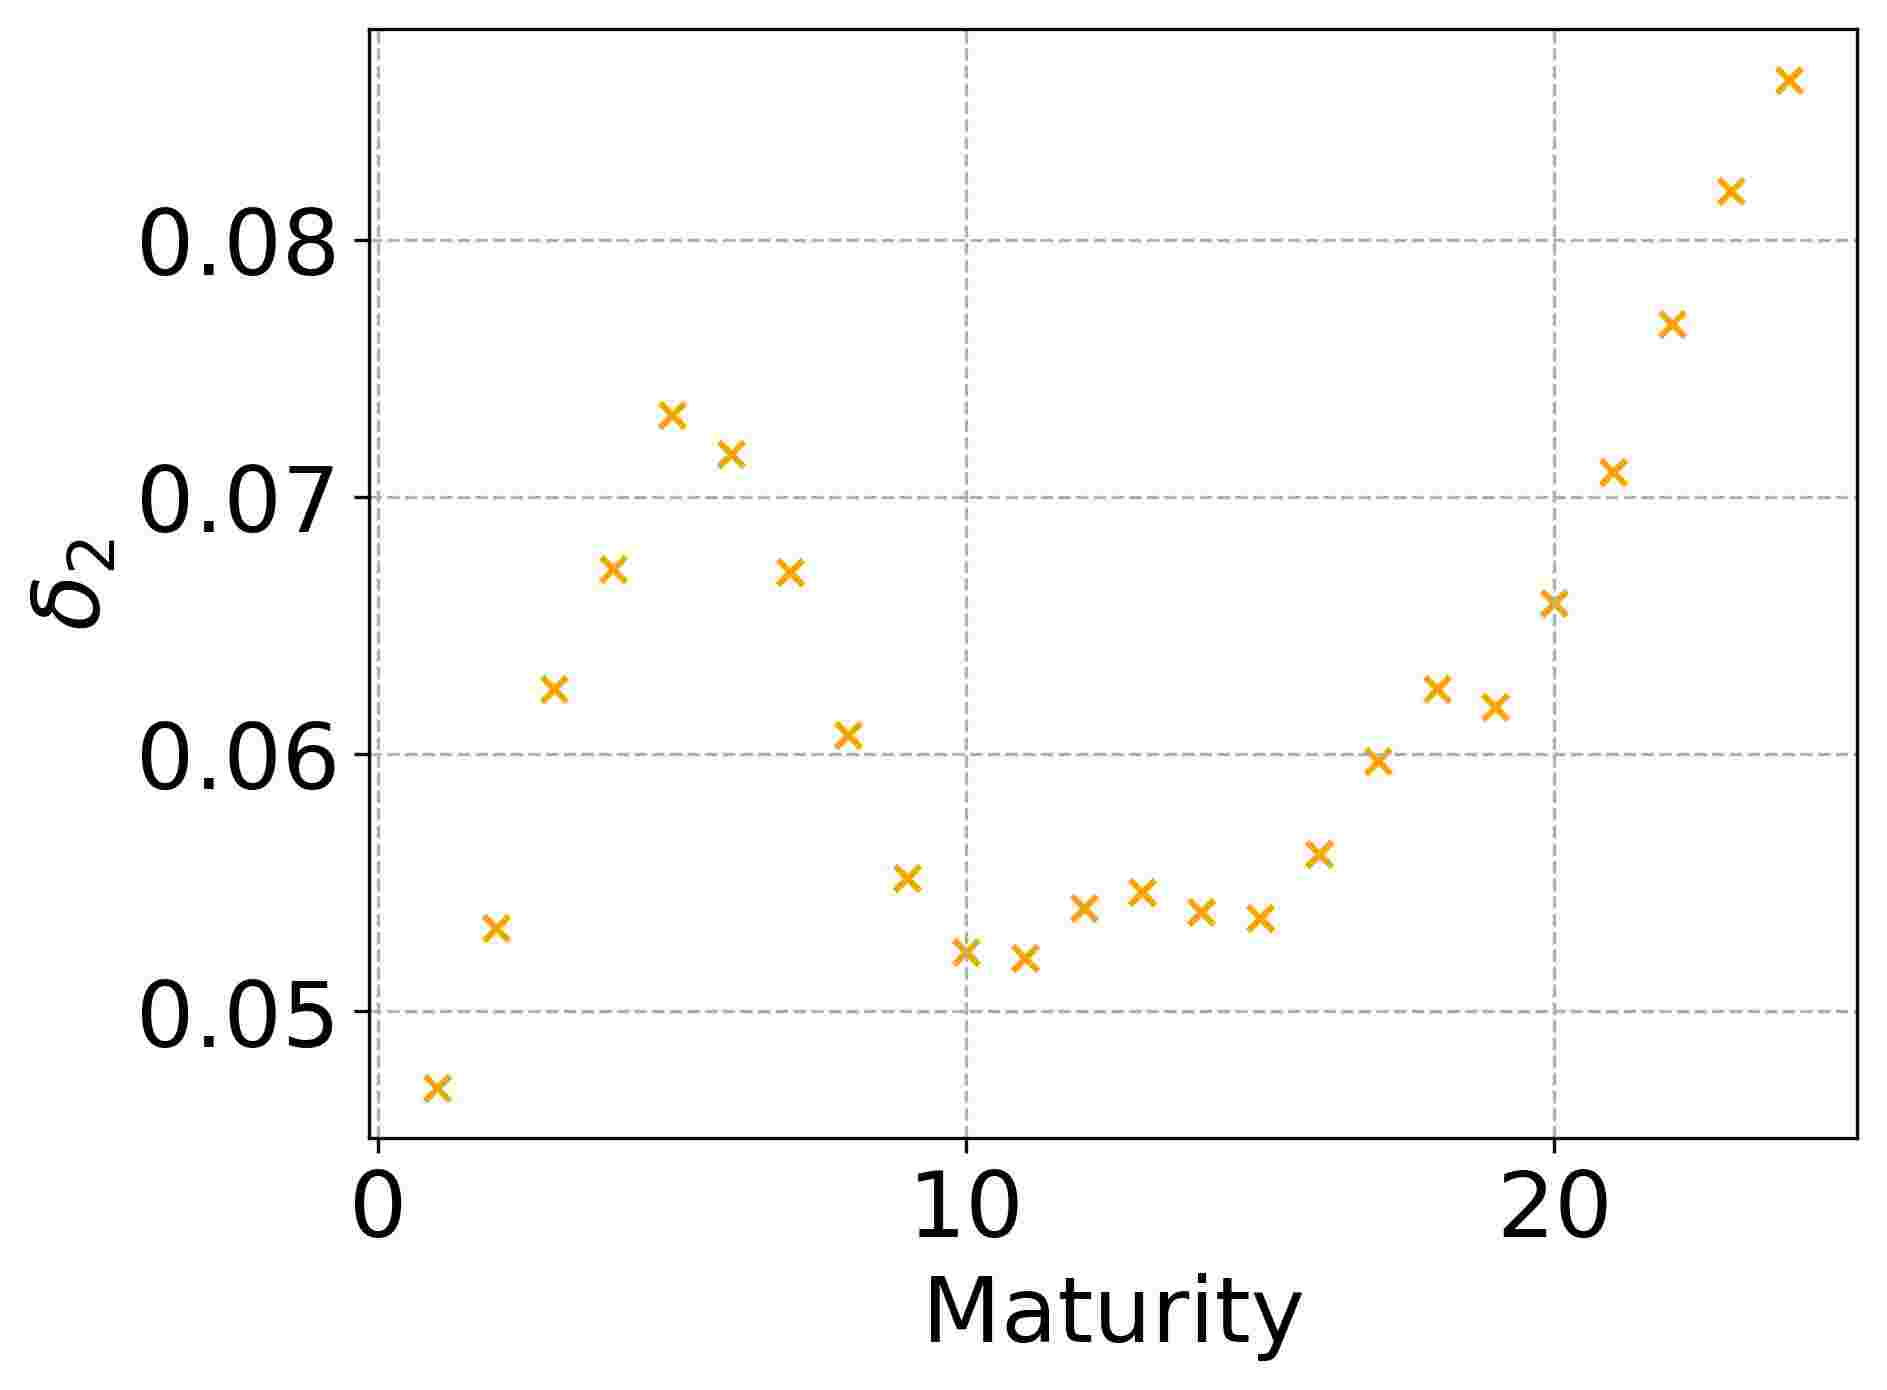
\includegraphics[width=0.23\linewidth]{STXE_delta_2.jpg}}

    \caption{Calibrated TSPL kernels parameters as a function of the time-to-maturity. The hyperparameters for the S\&P 500 are $(C_{R_1},C_{\Sigma},\lambda)=(250,1000,10^{-3})$ and those of the Euro Stoxx 50 are $(C_{R_1},C_{\Sigma},\lambda)=(10,1000,10^{-3})$.   }
\label{fig:pdv_params_tspl}
\end{figure}
\begin{figure}
    \centering
    \subfigure[$\beta_0$ (S\&P 500)]{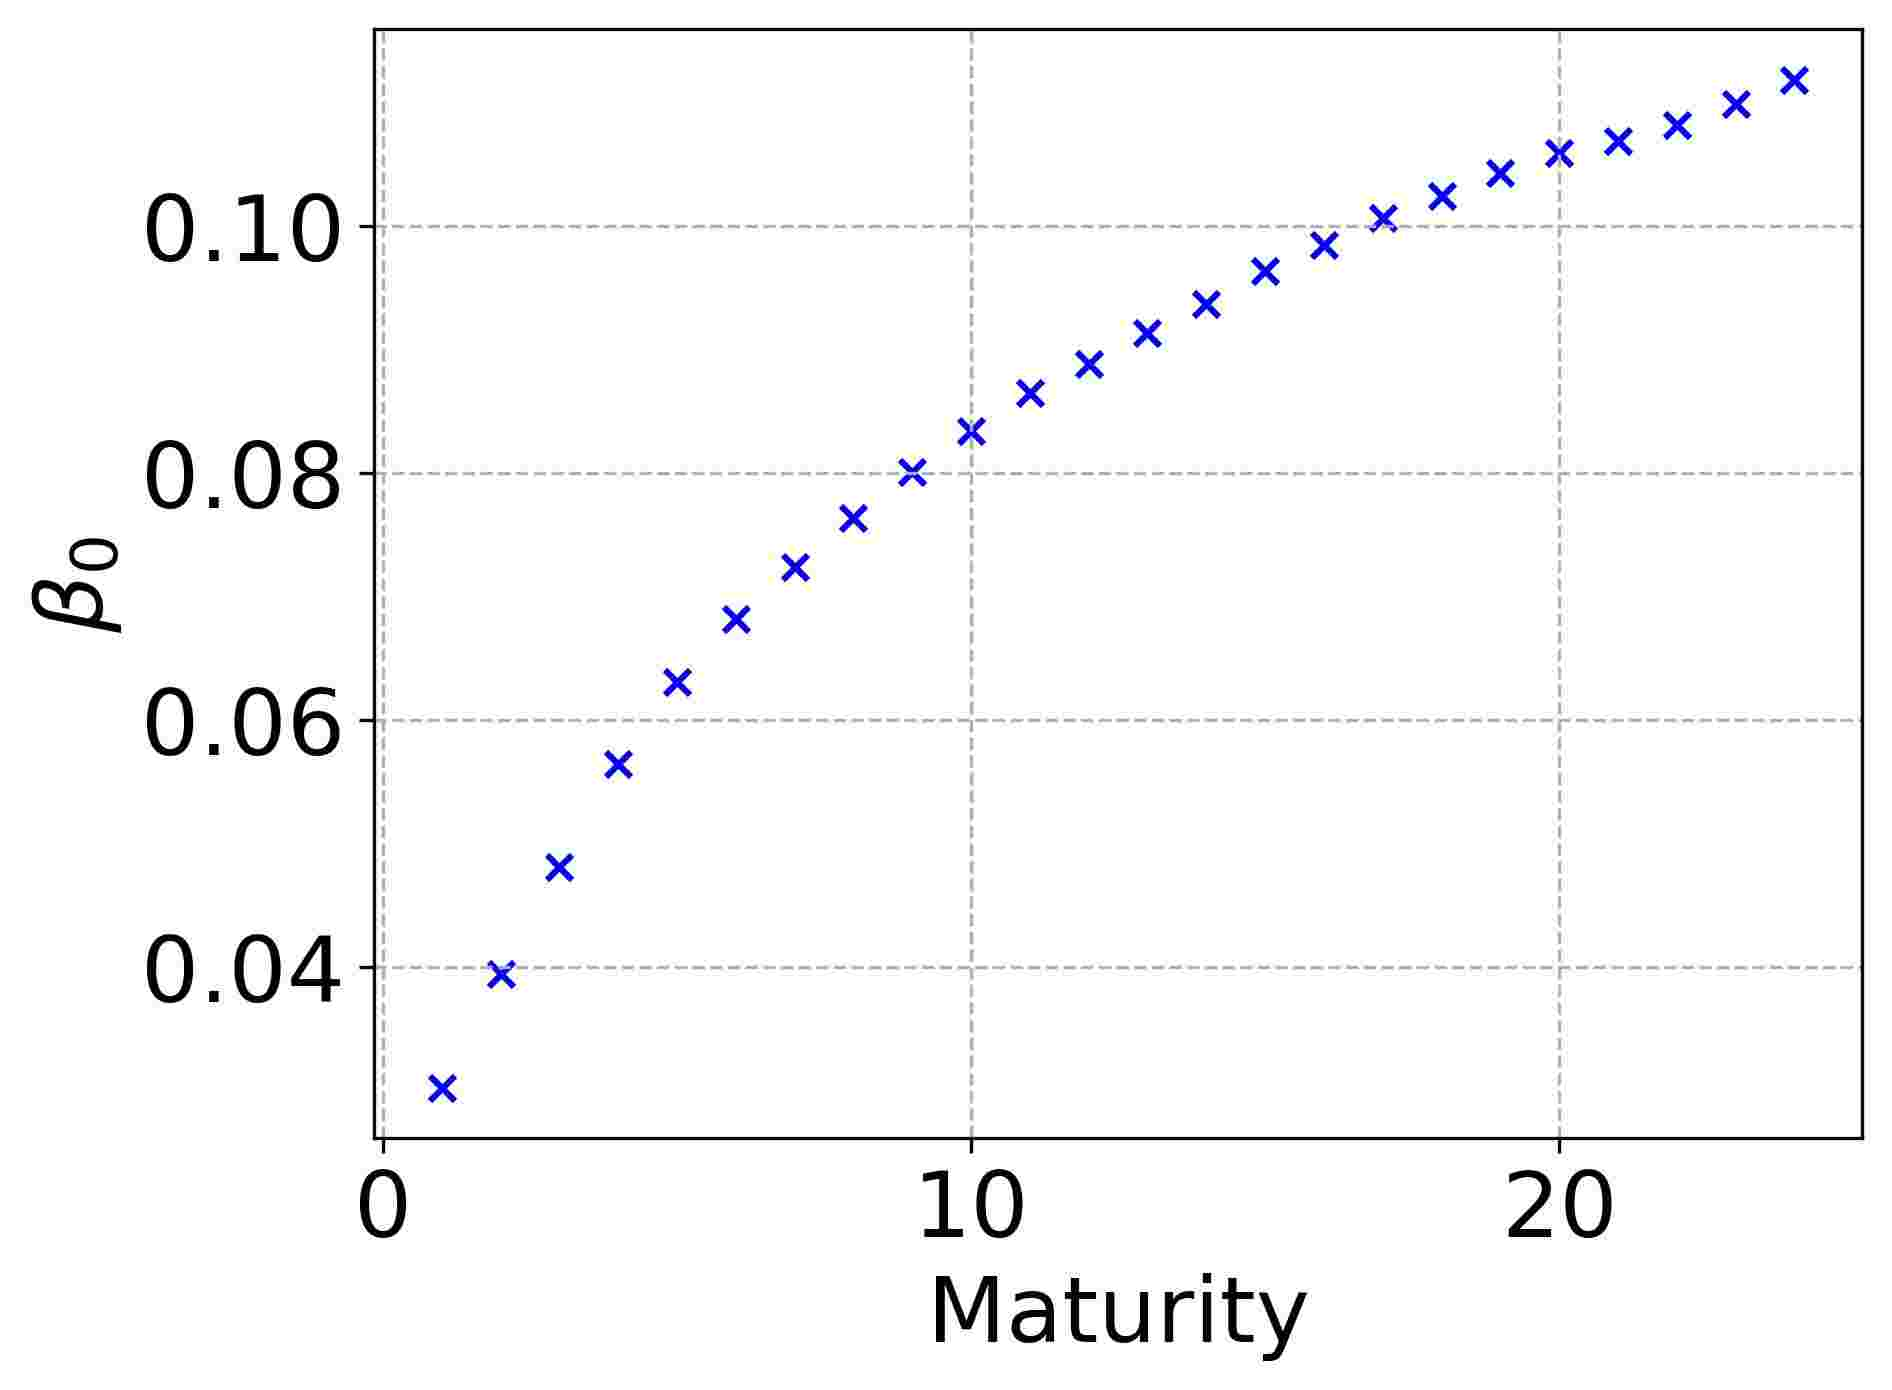
\includegraphics[width=0.3\linewidth]{SPX_beta_0.jpg}}
    \subfigure[$\beta_1$ (S\&P 500)]{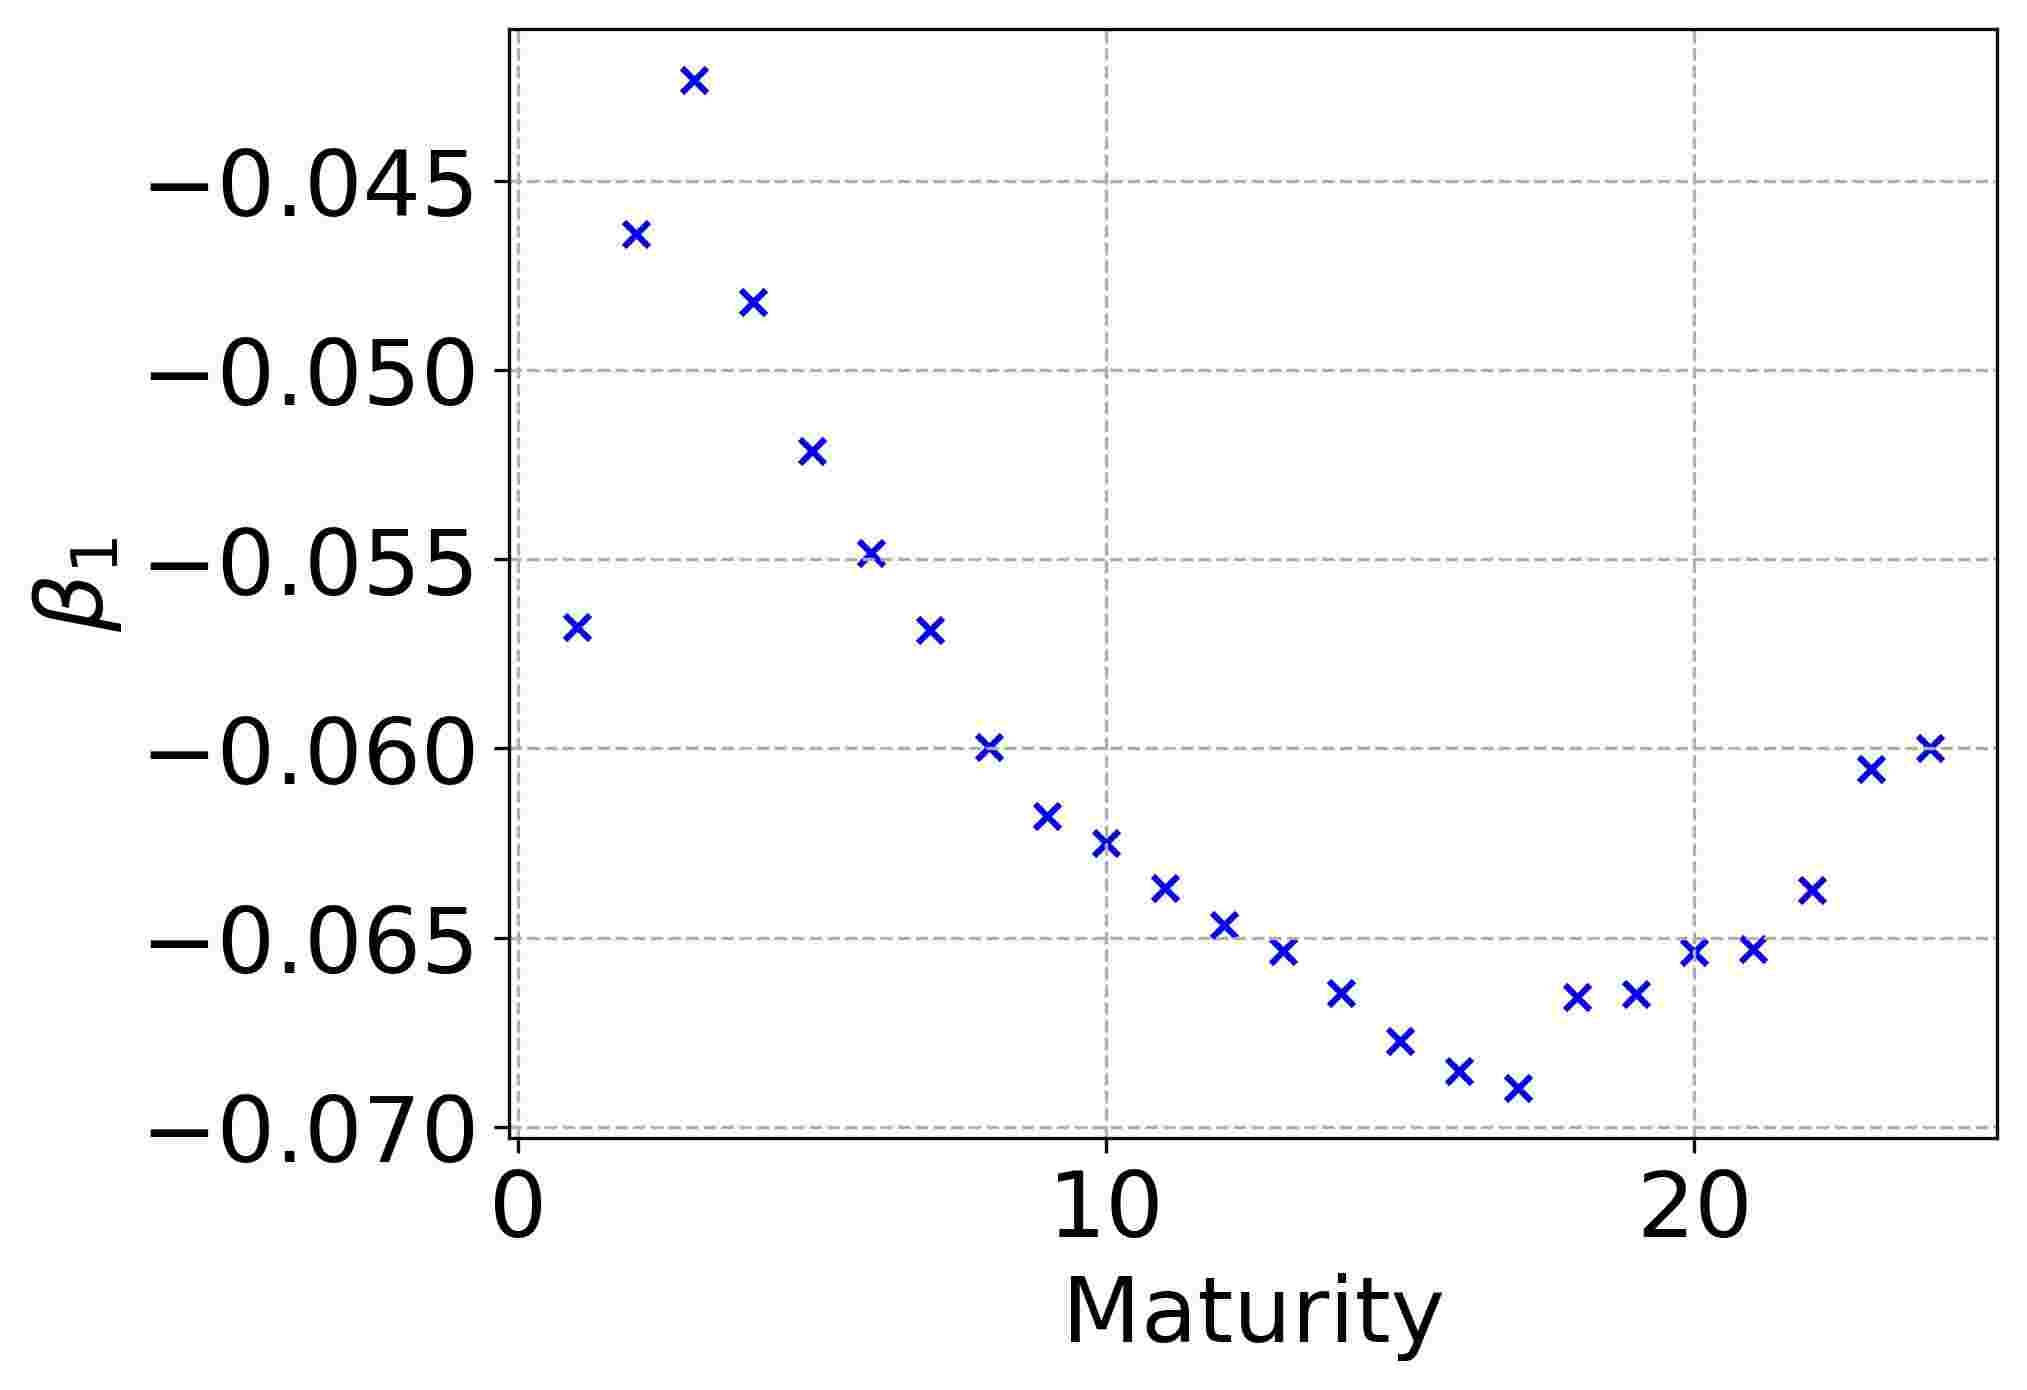
\includegraphics[width=0.3\linewidth]{SPX_beta_1.jpg}}
    \subfigure[$\beta_2$ (S\&P 500)]{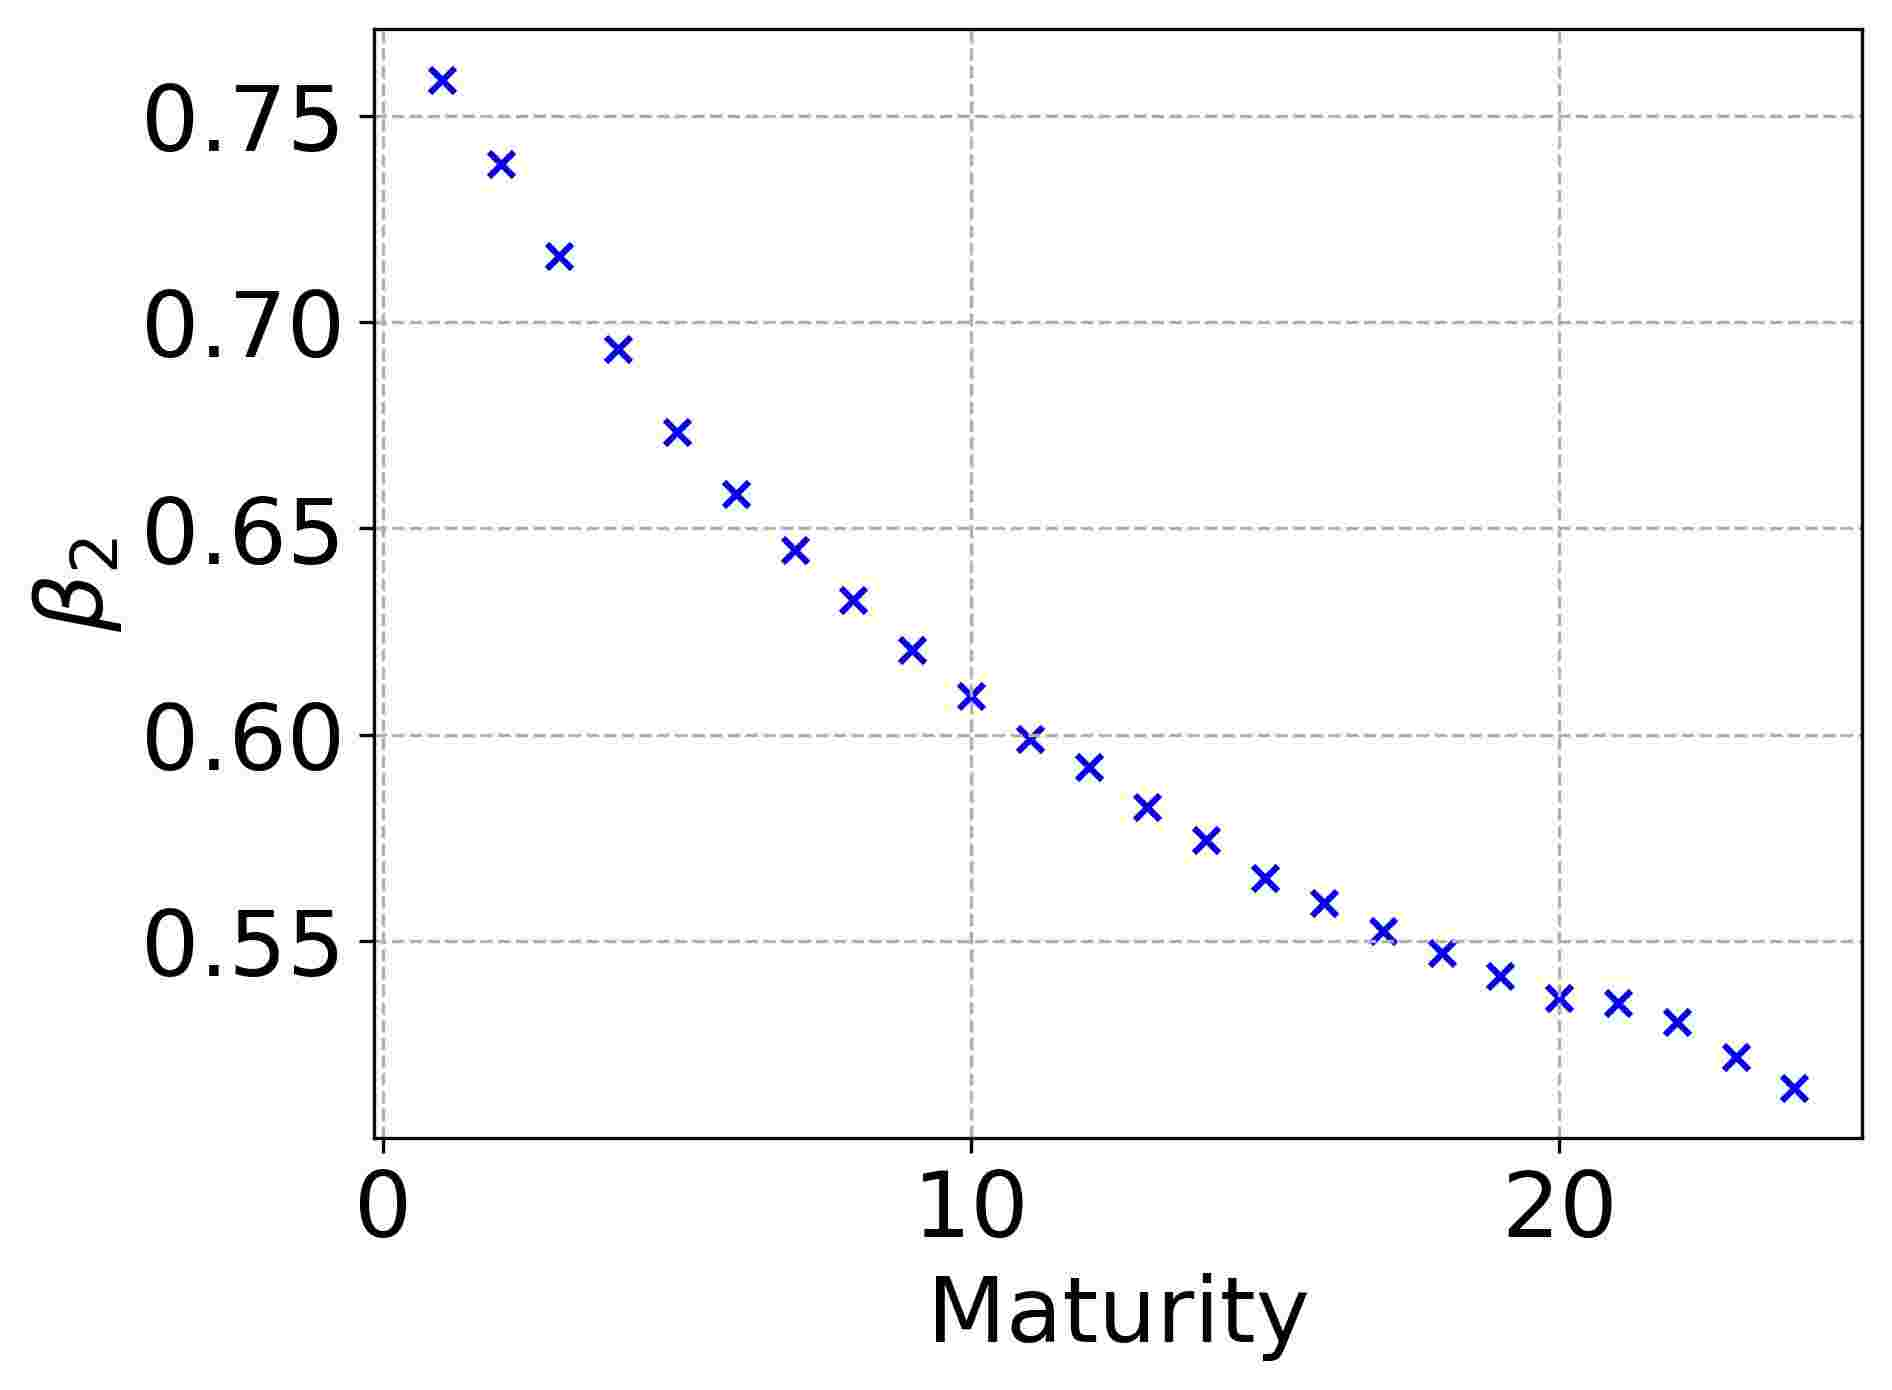
\includegraphics[width=0.3\linewidth]{SPX_beta_2.jpg}}
    \subfigure[$\beta_0$ (Euro Stoxx 50)]{ 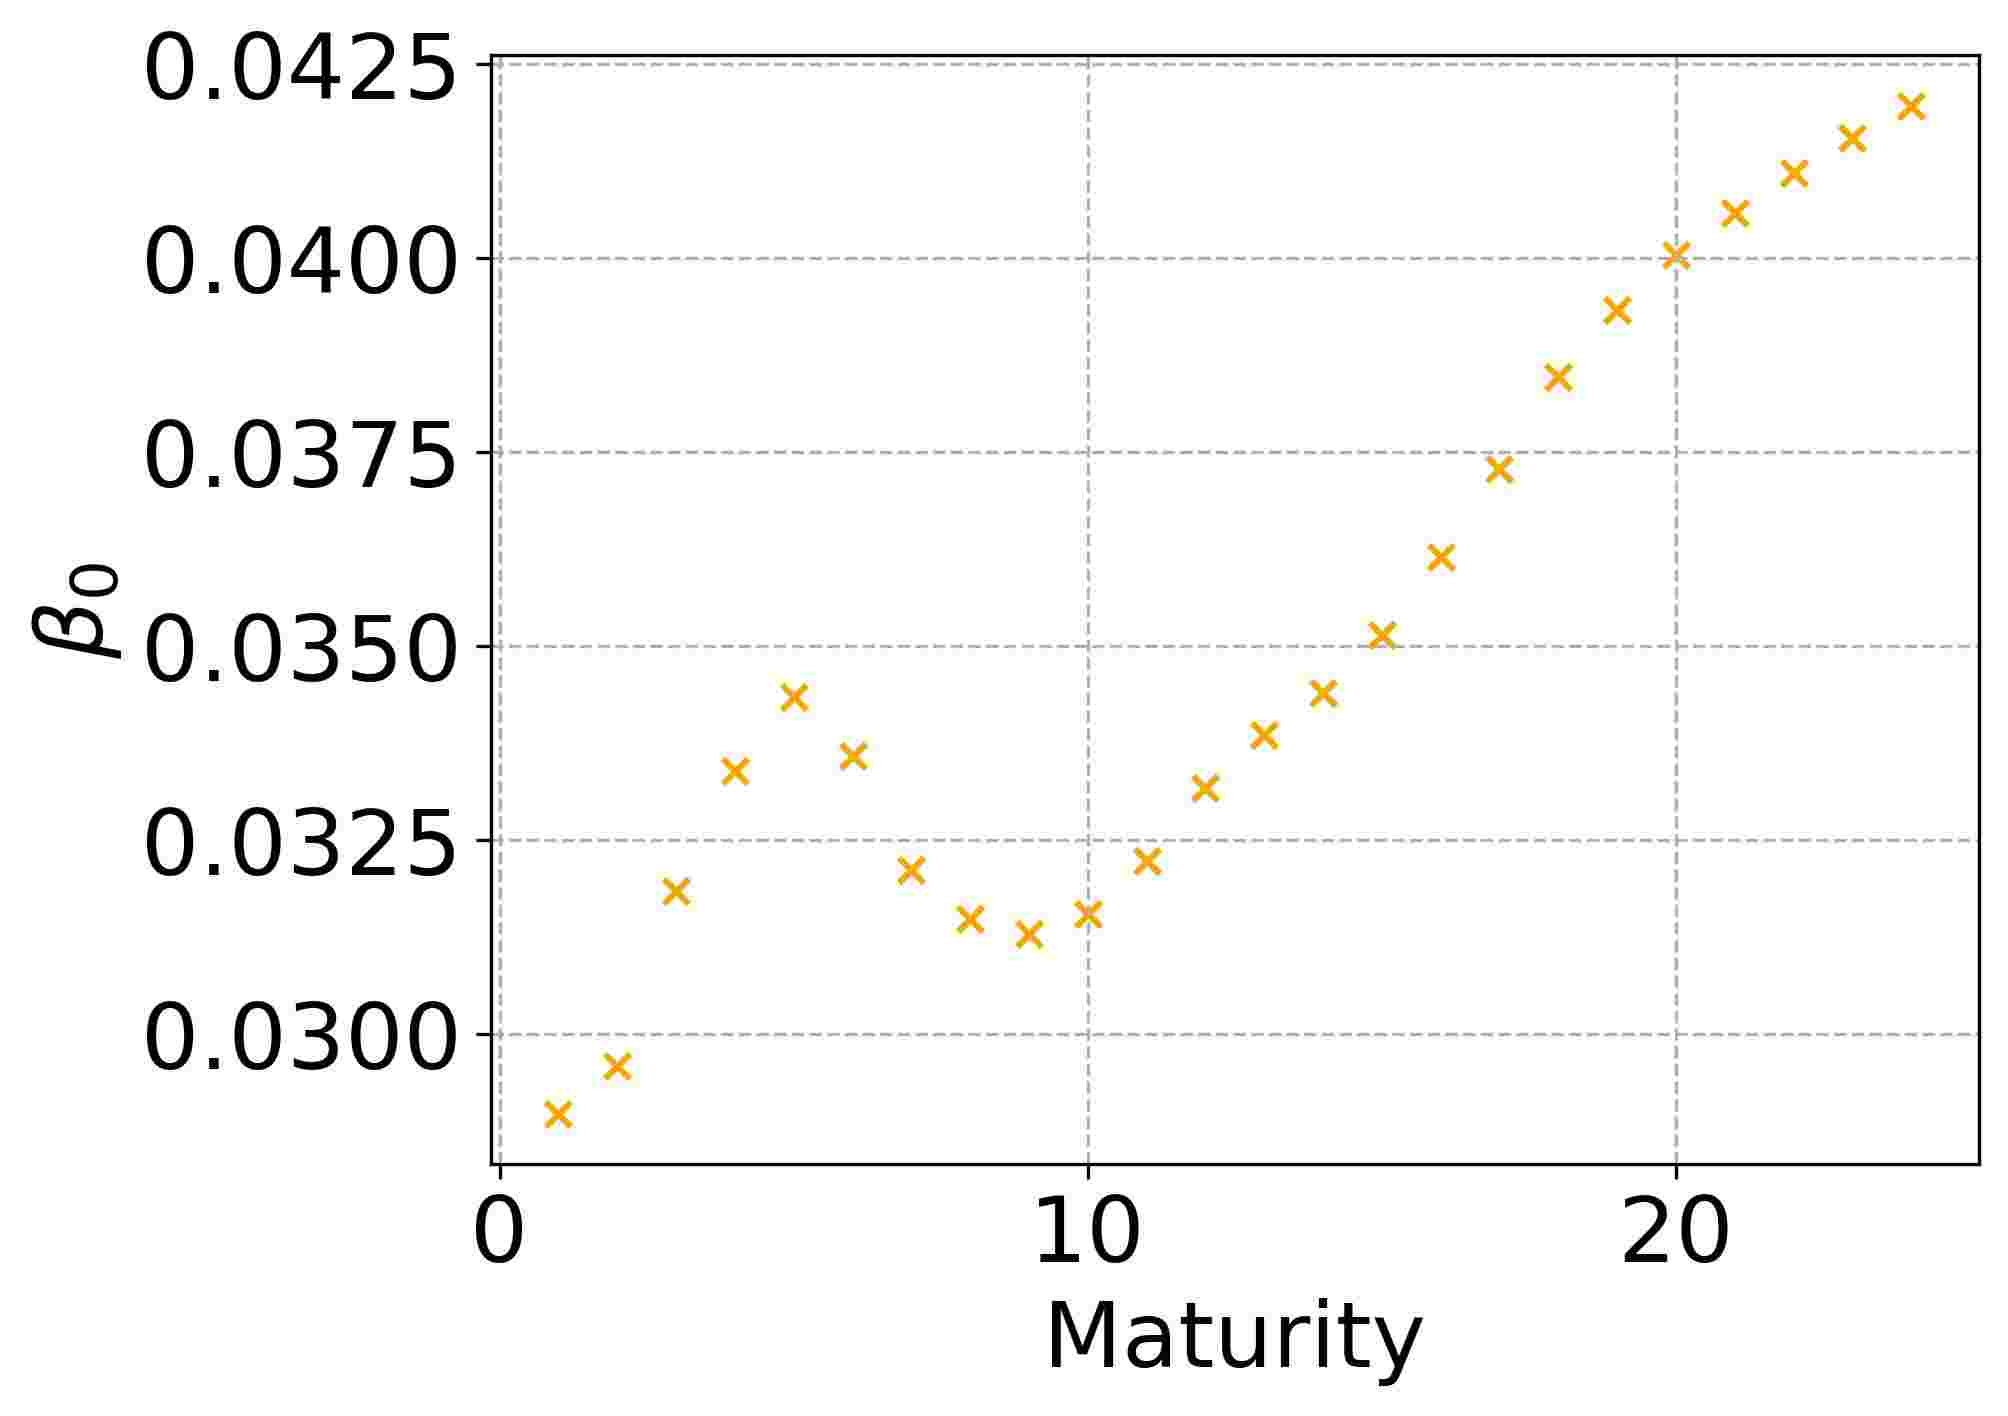
\includegraphics[width=0.3\linewidth]{STXE_beta_0.jpg}}
    \subfigure[$\beta_1$ (Euro Stoxx 50)]{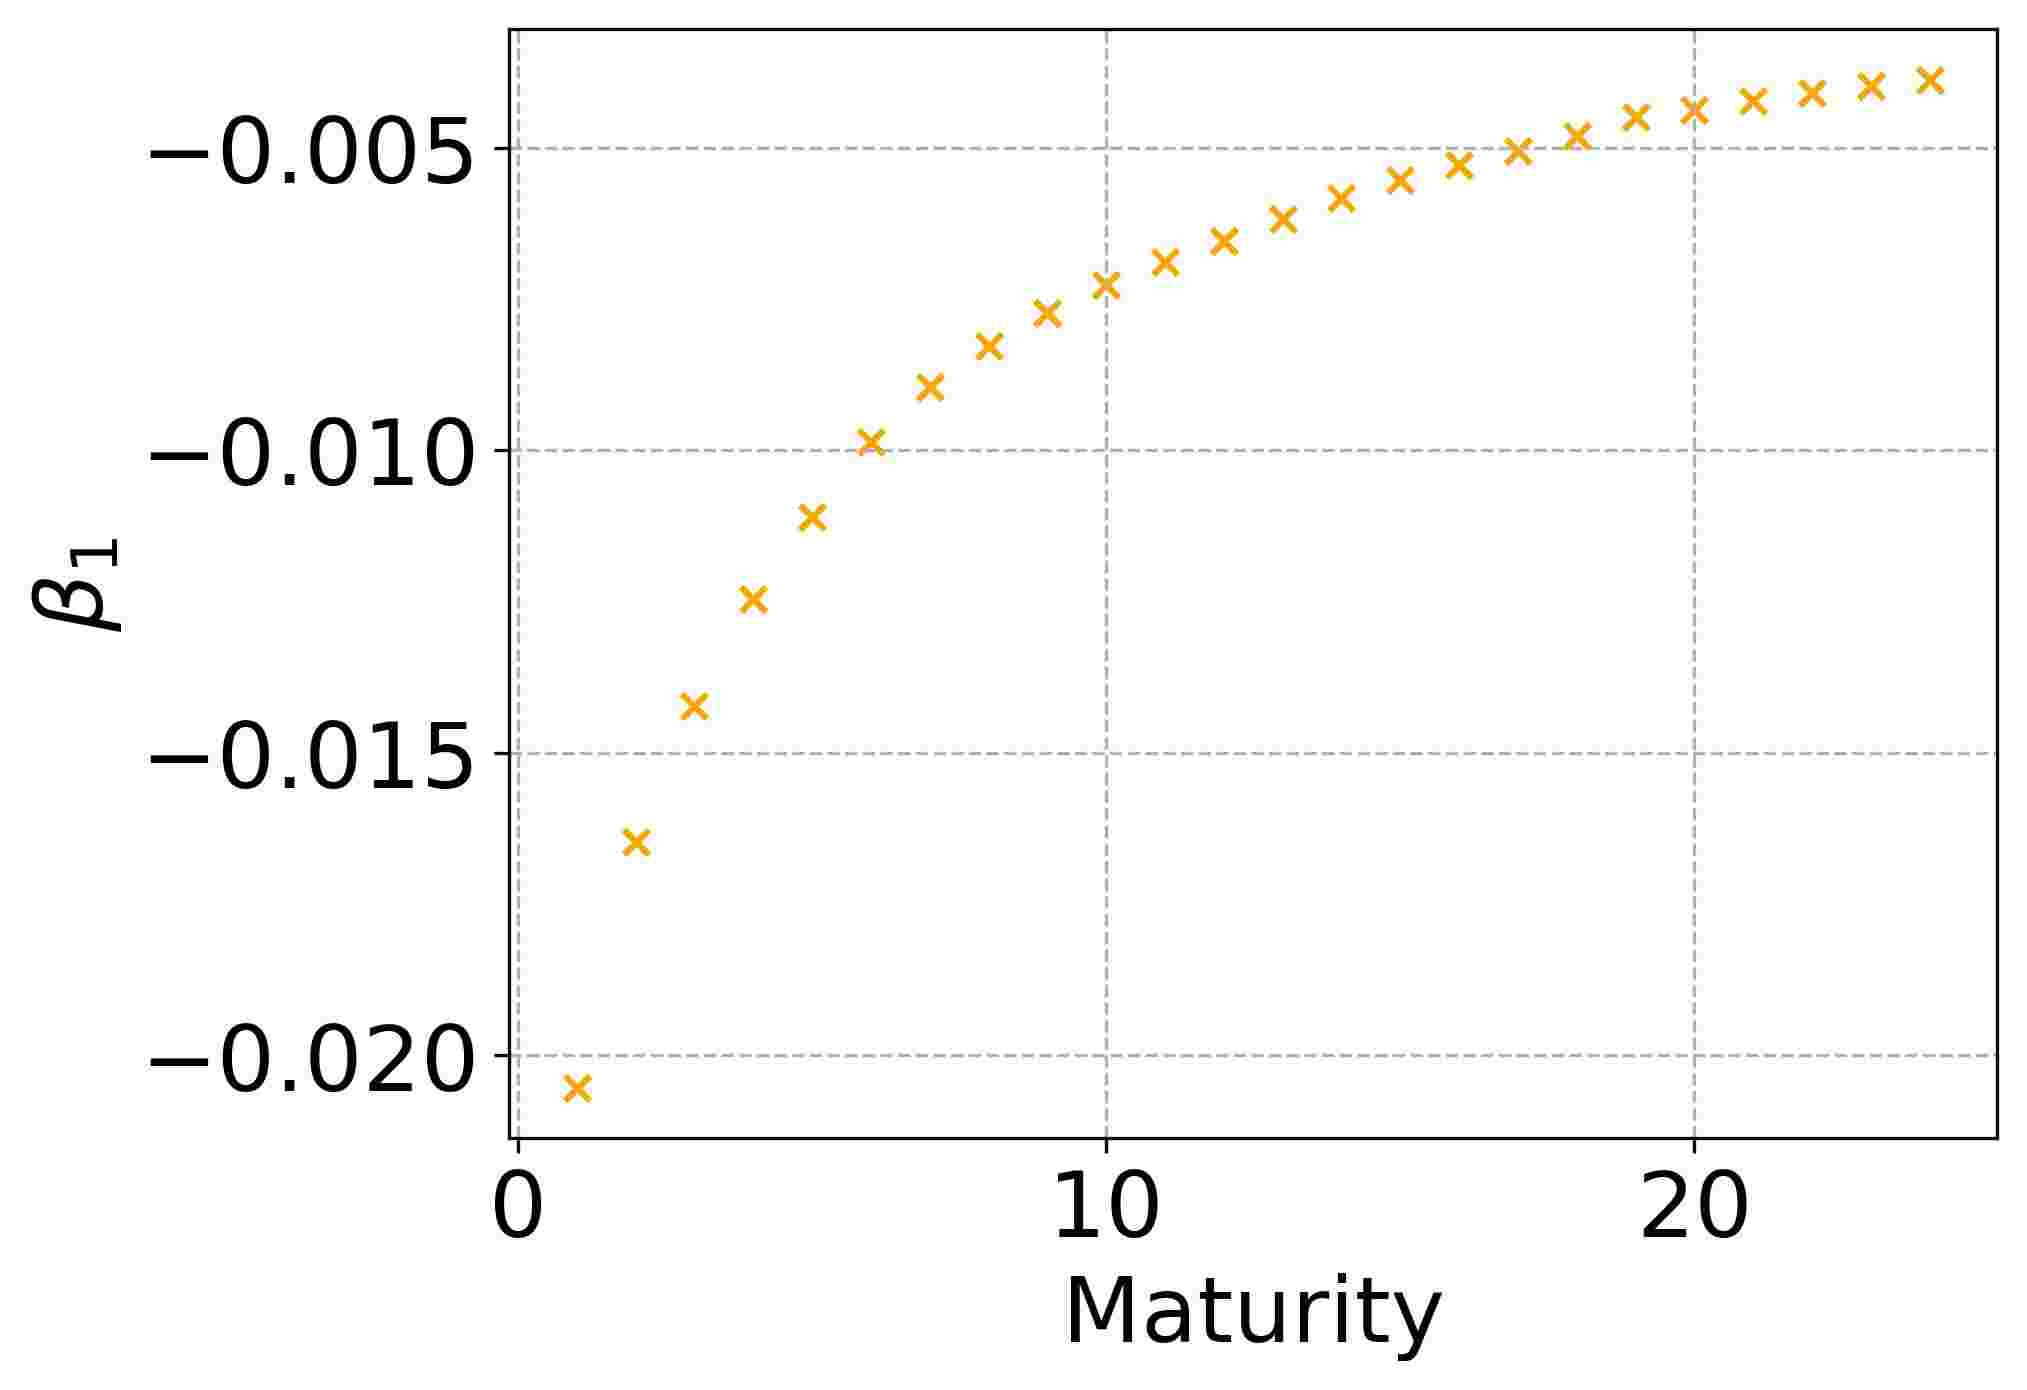
\includegraphics[width=0.3\linewidth]{STXE_beta_1.jpg}}
    \subfigure[$\beta_2$ (Euro Stoxx 50)]{ 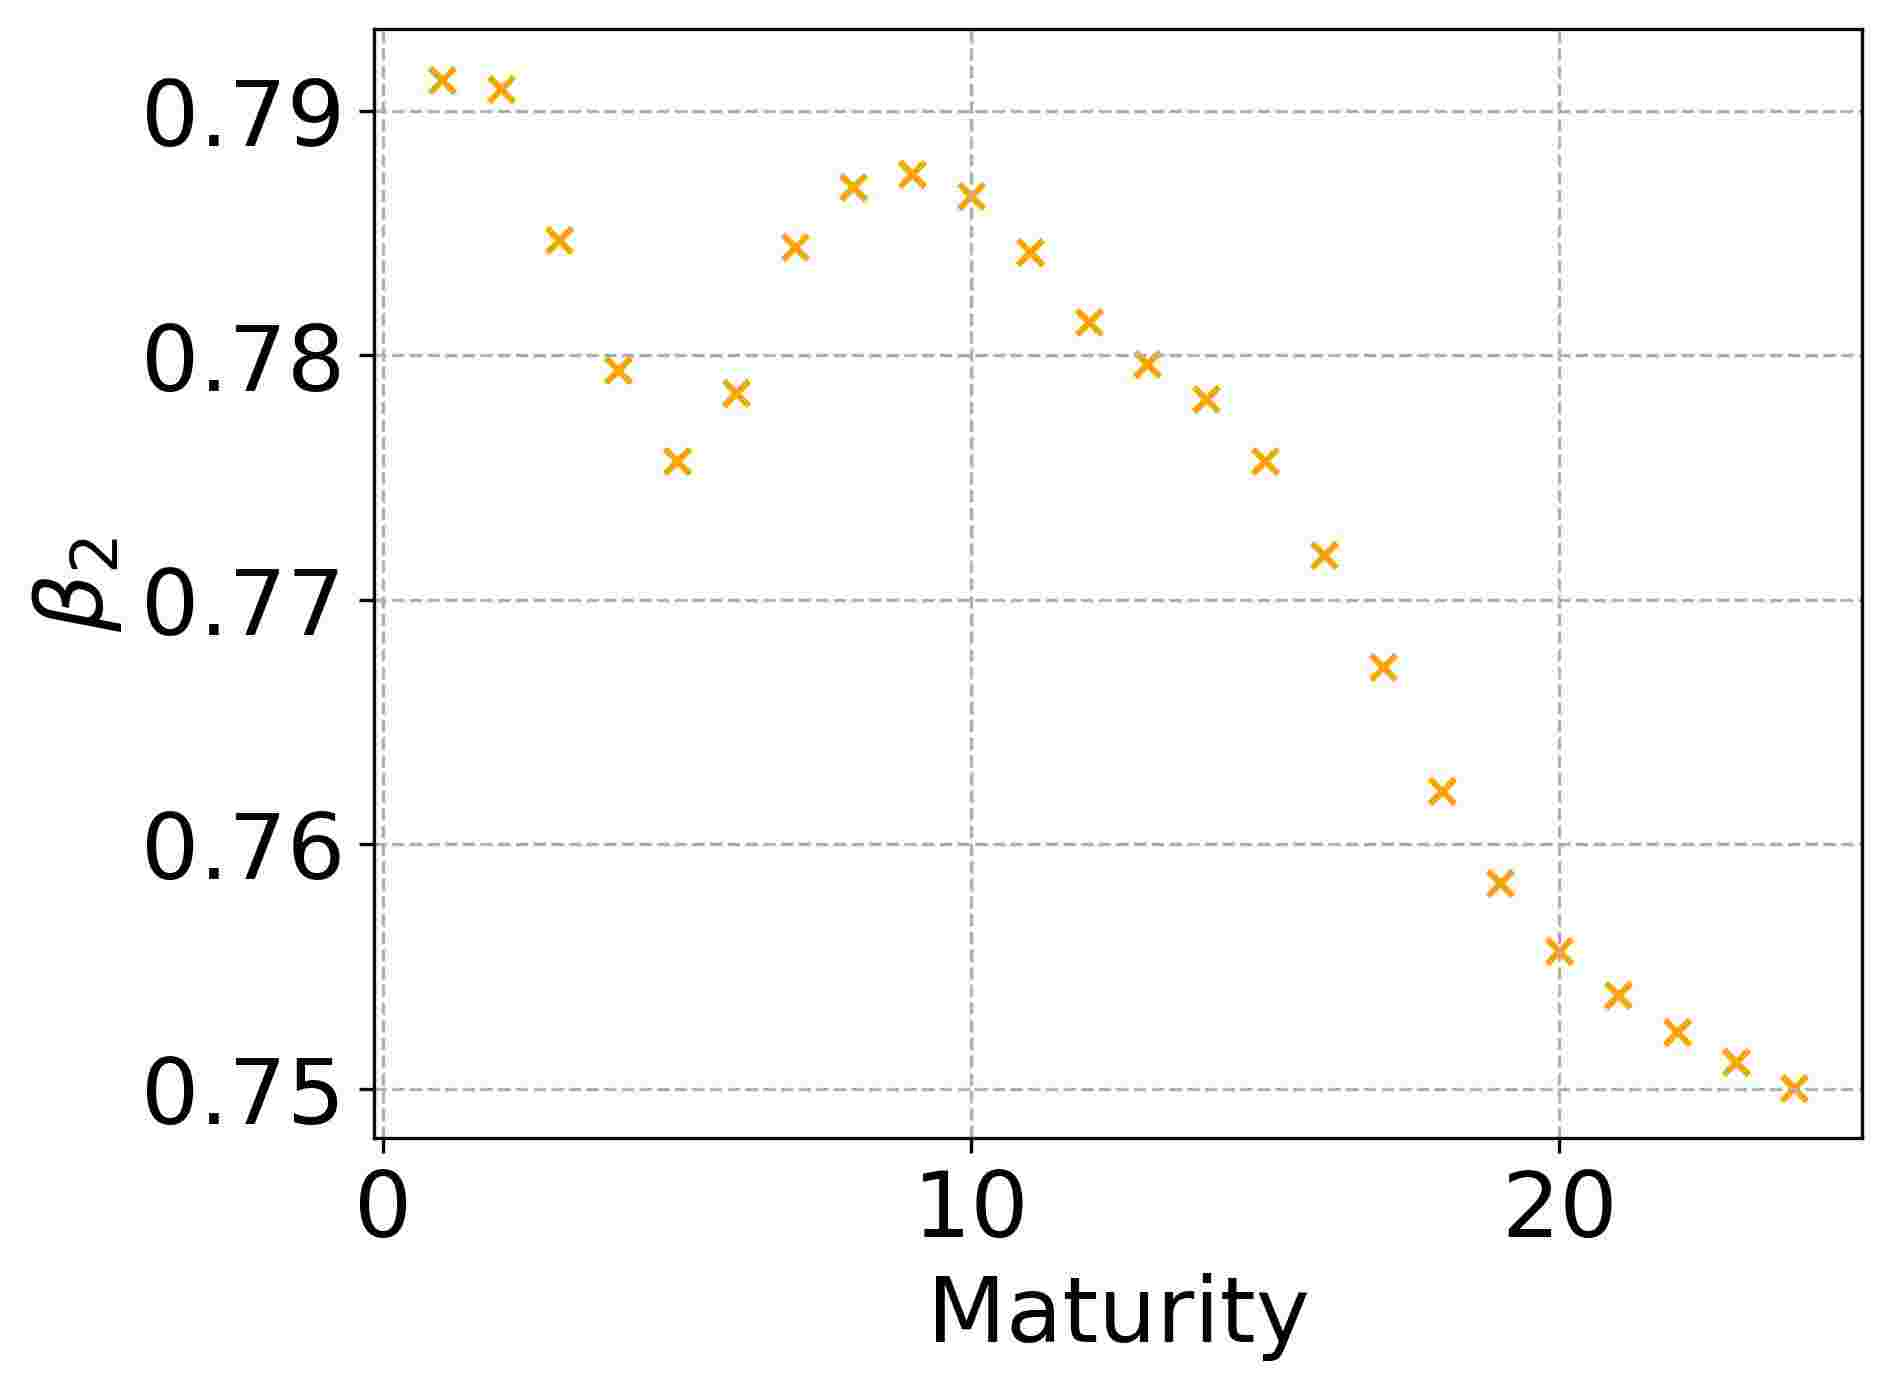
\includegraphics[width=0.3\linewidth]{STXE_beta_2.jpg}}
    \caption{Calibrated $\beta_0$, $\beta_1$ and $\beta_2$ as a function of the time-to-maturity. The hyperparameters for the S\&P 500 are $(C_{R_1},C_{\Sigma},\lambda)=(250,1000,10^{-3})$ and those of the Euro Stoxx 50 are $(C_{R_1},C_{\Sigma},\lambda)=(10,1000,10^{-3})$. }
\label{fig:pdv_params_lin_reg}
\end{figure}

\section{Absence of static arbitrage in the SSVI parameterization}\label{sec:ssvi_arbitrage}

Gatheral and Jacquier provide sufficient conditions for the SSVI to be free of arbitrage. These conditions are presented in the following theorem. 
\begin{theorem}[Corollary 4.1 from \cite{gatheral2014arbitrage}]
The SSVI is free of static arbitrage if the following conditions are satisfied:
\begin{enumerate}[(i)]
    \item $\partial_T \theta_T \ge 0$ for all $T>0$;
    \item $0\le \partial_{\theta}(\theta \varphi(\theta)) \le \frac{1}{\rho^2}\left(1+\sqrt{1-\rho^2} \right)\varphi(\theta)$ for all $\theta >0$;
    \item $\theta \varphi(\theta)(1+|\rho|)< 4$ for all $\theta >0$;
    \item $\theta\varphi(\theta)^2(1+|\rho|) \le 4$ for all $\theta >0$.
\end{enumerate}
\label{thm:ssvi_arbitrage}
\end{theorem}
\begin{remark}
    The conditions (i) and (ii) actually are necessary and sufficient conditions for the absence of calendar spread arbitrage for the SSVI. The condition (iii) with a non-strict inequality is a necessary condition for the absence of butterfly arbitrage but condition (iv) is only a necessary condition if $\theta \varphi(\theta)(1+|\rho|) = 4$. 
\end{remark}
\begin{remark}\label{rk:ssvi_weak_conditions}
    The conditions (ii), (iii) and (iv) can be weakened as follows:
    \begin{enumerate}[(i)]
        \setcounter{enumi}{1}
        \item $0\le \partial_{\theta}(\theta \varphi(\theta))\rvert_{\theta=\theta_T} \le \frac{1}{\rho^2}\left(1+\sqrt{1-\rho^2} \right)\varphi(\theta_T)$ for all $T >0$;
        \item $\theta_T \varphi(\theta_T)(1+|\rho|)< 4$ for all $T >0$;
        \item $\theta_T\varphi(\theta_T)^2(1+|\rho|) \le 4$ for all $T >0$.
    \end{enumerate}
    Note that these conditions are not necessarily equivalent to the ones in Theorem \ref{thm:ssvi_arbitrage} since $T\mapsto \theta_T$ is not necessarily a bijection from $\mathbb{R}_+^*$ to $\mathbb{R}_+^*$. 
\end{remark}
 The following propositions translate the sufficient conditions of Theorem \ref{thm:ssvi_arbitrage} for the three parameterizations of $\varphi$ introduced in Section \ref{sec:ssvi}. The proofs of Propositions \ref{prop:heston} and \ref{prop:power_law} can be found in Section 4 of \cite{gatheral2014arbitrage} while the one of Proposition \ref{prop:modified_power_law} is provided below. 
\begin{proposition}\label{prop:heston}
The SSVI-HL is free of static arbitrage if $\partial_T \theta_T \ge 0$ for all $T>0$ and $\lambda \ge (1+|\rho|)/4$. 
\end{proposition}
\begin{proposition}\label{prop:power_law}
    Assuming that $\partial_T \theta_T \ge 0$, we have the following cases:
    \begin{enumerate}[(i)]
        \item If $\gamma \in (0,1/2)$, there exists $\theta^* >0$ such that the SSVI-PL is free of static arbitrage if $\theta_T < \theta^*$ for all $T>0$.
        \item If $\gamma \in (1/2,1)$, there exists $\theta_1^*,\theta_2^*>0$ such that the SSVI-PL is free of static arbitrage if $\theta_2^* < \theta_T < \theta_1^*$ for all $T>0$.
        \item If $\gamma = 1/2$ and $\eta^2(1+|\rho|)\le 4$, there exists $\theta_1^*$ such that the SSVI-PL is free of static arbitrage if $\theta_T < \theta_1^*$ for all $T>0$. 
    \end{enumerate}
\end{proposition}
\begin{proposition}\label{prop:modified_power_law}
    Assuming that $\partial_T \theta_T \ge 0$, we have the following cases:
\begin{enumerate}[(i)]
    \item If $\gamma \in (0,1/2)$ and $\eta (1+|\rho|) \le 4$, there exists $\theta^*>0$ such that the SSVI-MPL is free of static arbitrage if, for all $T>0$, $\theta_T\ge \theta^*$.
    \item If $\gamma \in (1/2,1)$, the SSVI-MPL is free of static arbitrage for $\eta(1+|\rho|) \le 4$ and $(1-2\gamma)\varphi(1-2\gamma)^2(1+|\rho|)\le 4$. 
    \item If $\gamma=1/2$, the SSVI-MPL is free of static arbitrage for $\eta^2 (1+|\rho|) \le 4$.\label{prop:pssvi_no_arbitrage}
\end{enumerate}
\begin{proof}
    We have $\partial_{\theta}(\theta\varphi(\theta)) = \frac{1-\gamma}{1+\theta}\varphi(\theta)$, thus $0< \partial_{\theta}(\theta\varphi(\theta)) < \varphi(\theta)$ and condition (ii) of Theorem \ref{thm:ssvi_arbitrage} is satisfied since $\frac{1}{\rho^2}\left(1+\sqrt{1-\rho^2} \right) \ge 1$ for $\rho \in (-1,1)$. This shows also that $\theta \mapsto \theta\varphi(\theta)$ is strictly increasing. Since $\lim_{\theta \to +\infty} \theta\varphi(\theta) = \eta$, we deduce that condition (iii) is equivalent to $\eta(1+|\rho|)\le 4$. Finally, for condition (iv), we have:
\begin{equation}
    \partial_{\theta}(\theta\varphi(\theta)^2) = \frac{\eta^2}{\theta^{2\gamma}(1+\theta)^{3-2\gamma}}(1-\theta-2\gamma).
\end{equation}
Therefore, we have the following cases:
\begin{itemize}
    \item If $\gamma \in (1/2,1)$, then $\theta\mapsto \theta\varphi(\theta)^2$ is stricly decreasing on $\mathbb{R}_+$ with $\lim_{\theta \to 0} \theta\varphi(\theta)^2 = +\infty$ and $\lim_{\theta \to +\infty}\theta\varphi(\theta)^2 = 0$. Thus according to Remark \ref{rk:ssvi_weak_conditions}, if $\eta(1+|\rho|)\le 4$ then the SSVI is free of static arbitrage if $\theta_T \ge \theta^*$ for all $T>0$ where $\theta^*$ satisfies $\theta^*\varphi(\theta^*)^2 = 4/(1+|\rho|)$. 
    \item If $\gamma \in (0,1/2)$, then $\theta\mapsto \theta\varphi(\theta)^2$ is stricly increasing on $(0,1-2\gamma)$ and then stricly decreasing on $(1-2\gamma,+\infty)$, thus it is bounded from above by $(1-2\gamma)\varphi(1-2\gamma)^2$. We deduce that the SSVI is free of static arbitrage for $\eta(1+|\rho|)\le 4$ and $(1-2\gamma)\varphi(1-2\gamma)^2(1+|\rho|)\le 4$.
    \item If $\gamma = 1/2$, then $\theta\mapsto \theta\varphi(\theta)^2$ is stricly decreasing on $\mathbb{R}_+$ and bounded from above by $\eta^2$. We deduce that the SSVI is free of static arbitrage for $\eta(1+|\rho|)\le 4$ and $\eta^2(1+|\rho|) \le 4$ which is equivalent to $\eta^2(1+|\rho|) \le 4$ since for $\eta < 1$, we have $\eta(1+|\rho|)\le 4$ for all $\rho \in [-1,1]$. 
\end{itemize}
\end{proof}
\end{proposition}
\begin{remark}
Note that different sufficient conditions could be found for guaranteeing the absence of static arbitrage by restricting the time-to-maturity $T$ to some subset of $\mathbb{R}_+^*$. Since it is not very satisfying to have an IVS parameterization that could be arbitrable for some time-to-maturities, we looked as much as possible for conditions that do not restrict the values of $T$. 
\end{remark}



\section{SSVI calibration results}\label{sec:ssvi_calibration_results}
In this section, we study the fitting accuracy of the SSVI parameterization for the three choices of the function $\varphi$ introduced in Section \ref{sec:ssvi} on the historical IVSs that we presented in Section \ref{sec:data}. Let us recall that our historical IVSs are already the result of an interpolation of raw data as pointed out in Section \ref{sec:data}. Therefore, the calibration results that we present in this section may differ from those obtained using raw data or data interpolated with a method different from that of our data providers. Moreover, as already noted by \cite{cont2022simulation}, our historical IVSs are not necessarily arbitrage-free because of these interpolations. Procedures such as the ones of \cite{davis2007range} or \cite{cohen2020repairing} allow to detect arbitrages in a finite set of prices of European call options given the forward prices. Our database does not contain short rates data or forward prices data so we cannot use these procedures. Since calendar spread arbitrages are equivalent to the total implied variance being non-decreasing in time-to-maturity, we remove the IVSs (we recall that our data sets contain one IVS per business day) such that there is at least one crossing between the linearly interpolated total implied variances of two adjacent time-to-maturities. IVSs with butterfly arbitrages (if any) are not removed as the condition in terms of total implied variance is much more complicated to verify. In total, 0.8\% (resp. 5.6\%) of the IVSs are removed from the S\&P 500 (resp. Euro Stoxx 50) data set.  \\

To measure the fitting accuracy, we calibrate the SSVI for each day of our data sets without calendar spread arbitrages and for each parametric form of $\varphi$ by solving the following minimization problem using the \texttt{minimize} function with the SLSQP algorithm from the \texttt{scipy} Python package:
\begin{equation}\label{eq:ssvi_calibration}
    \begin{array}{rrrcllr}
    \displaystyle\min_{\Theta=((\theta_{T_i})_{i=1,\dots,M},\rho,\Pi_{\varphi})} & \multicolumn{5}{c}{\displaystyle\sum_{i=1}^M\sum_{k\in\mathcal{K}_{T_i}} \phi(k) \left(\sigma_{Mkt}(k,T_i) - \sigma_{SSVI}(k,T_i;\Theta)\right)^2 } \\
        \text{s.t.} & \theta_{T_1} & \ge & 0 & & \\
    &\theta_{T_{i+1}} &\ge &\theta_{T_i} & \text{for } 1\le i \le M-1 &  \\
    & (\rho,\Pi_{\varphi}) & \in & C_{\varphi}. &&
        \end{array}
\end{equation}


We used the following notations:
\begin{itemize}
    \item $\Pi_{\varphi}$ is the vector of the parameters in $\varphi$: only $\lambda$ for the SSVI-HL and $(\eta,\gamma)$ for the SSVI-PL and the SSVI-MPL. 
    \item $T_1<T_2<\dots < T_M$ is the set of time-to-maturities and $\mathcal{K}_T$ is the set of log-strikes for the time-to-maturity $T$. Note that for the S\&P 500 data set, we have the implied volatilities for forward moneynesses between 0.6 and 1.4. In order to keep only the most liquid options and for consistency with the Euro Stoxx 50 data set, we only consider the forward moneynesses for which the (call) Black-Scholes delta is between 0.1 and 0.9.
    \item $\phi(k)$ is the standard normal density function evaluated in the log-strike $k$. This weighting function allows to give more weight to the replication of the implied volatilities that are close to the money. Another choice based on the Black-Scholes vega has been considered but we did not notice any improvement.
    \item $\sigma_{Mkt}$ is the market implied volatility. 
    \item  $\sigma_{SSVI}(\cdot,\cdot;\Theta)$ is the SSVI implied volatility associated to the parameter vector $\Theta=((\theta_{T_i})_{i=1,\dots,M},\rho,\Pi_{\varphi})$.
    \item $C_{\varphi}$ is given by: 
    \begin{itemize}
        \item[--]  $C_{\varphi} = \{ (\rho,\lambda) \in (-1,1)\times \mathbb{R}_+^* : \lambda \ge (1+|\rho|)/4 \}$ for the SSVI-HL,
        \item[--]  $C_{\varphi} = \{(\rho,\eta,\gamma) \in (-1,1)\times \mathbb{R}_+^*\times (0,1) : \eta^2(1+|\rho|) \le 4 \text{ if } \gamma = 1/2 \}$ for the SSVI-PL and,
        \item[--] \begin{equation*}
            C_{\varphi} = \left\{
            \begin{array}{ll}
                \multicolumn{2}{l}{(\rho,\eta,\gamma)\in(-1,1)\times \mathbb{R}_+^*\times (0,1) :} \\
                \eta (1+|\rho|) \le 4 & \text{ if } \gamma < 1/2 \\
                \eta (1+|\rho|) \le 4 \text{ and } (1-2\gamma)\varphi(1-2\gamma)^2(1+|\rho|)\le 4 & \text{ if } \gamma >1/2 \\
                \eta^2(1+|\rho|) \le 4 & \text{ if } \gamma = 1/2 
            \end{array}
            \right\}
        \end{equation*}
        for the SSVI-MPL. 
    \end{itemize}
\end{itemize}
\begin{remark}
The constraints in the above minimization problem do not guarantee the absence of static arbitrage for the power-law and the modified power-law parameterizations since only the constraints involving $\rho$, $\eta$ and $\gamma$ are included as well as the non-decreasing property of $T\mapsto \theta_T$. The reason for this choice is the fact that there is no closed-form expression for $\theta^*$, $\theta_1^*$ and $\theta_2^*$ so the addition of the constraints involving these terms would strongly complexify the numerical optimization. By the end of this section, the study will be restricted to the SSVI-MPL parameterization with $\gamma=1/2$ (for which there is no constraint involving $\theta^*$, $\theta_1^*$ or $\theta_2^*$) so this choice is impact-free. 
\end{remark}
\begin{remark}
We use in practice the change of variable $(\tilde{\theta}_T)_{i=1,\dots,M}$ where $\tilde{\theta}_{T_1}=\theta_{T_1}$ and $\tilde{\theta}_{T_{i}} = \theta_{T_i}-\theta_{T_{i-1}}$ for $i \in \{2,\dots,M\}$ since it allows to transform the second inequality constraints in the minimization problem (\ref{eq:ssvi_calibration}) in bounds constraints: $\tilde{\theta}_{T_i} \ge 0$ for $2\le i \le M$. 
\end{remark}
The initial guess for each parameter is provided in Table \ref{tab:initial_guess}. The average relative errors (without weighting) between the market implied volatilities and the SSVI implied volatilities for each day of our data sets are presented in Figure \ref{fig:ssvi_relative_error}. It appears clearly that the Heston-like parameterization performs very poorly in comparison to the two others parameterizations. This results from the fact that, in the Heston-like parameterization, the function $\varphi$ is bounded from above by $1/2$ which constraints strongly the shape of the IVS. The power-law and the modified power-law parameterizations achieve essentially the same accuracy which is very stable over time. In particular, we do not observe a decrease of the fitting quality during the Covid-19 crisis.
\begin{table}[h]
    \centering
    \caption{Initial guesses provided to the optimization routine. }
    \label{tab:initial_guess}
    \begin{tabular}{@{}ccccc@{}}
    \toprule
    $(\theta_{T_i})_{i=1,\dots,M}$ & $\rho$ & $\lambda$ & $\eta$ & $\gamma$ \\ \midrule
    $(\sigma_{Mkt}(0,T_i)^2T_i)_{i=1,\dots,M}$ & -0.5 & 1      & 1   & 0.25   \\ \bottomrule
    \end{tabular}
\end{table}
\begin{figure}[h]
    \centering
    \subfigure[S\&P 500]{\includegraphics[width=0.45\linewidth]{SPX_SSVI_calibration.jpg}}
    \subfigure[Euro Stoxx 50]{\includegraphics[width=0.45\linewidth]{SX5E_SSVI_calibration.jpg}}
    \caption{Average relative errors between the market implied volatilities and the SSVI implied volatilities after the calibration.}
\label{fig:ssvi_relative_error}
\end{figure}

\section{Hyperparameters of the PDV model calibrated on the parsimonious SSVI parameters}\label{sec:hyperparams_ssvi}
Similarly to the study in Appendix \ref{sec:influence_cutoff}, for each parameter of the parsimonious SSVI, we run a 10-fold blocked cross-validation on the train set to determine the optimal hyperparameters $C_{R_1}$, $C_{\Sigma}$ and $\lambda$ in the grid $\{5,10,25,50,100,250,500,1000,1500,2000,2500\}^2\times \{10^{-6},10^{-5},\dots,10^{-1}\}$. The obtained hyperparameters are given in Table \ref{tab:pssvi_hyperparameters}
\begin{table}[h]
    \centering
    \caption{Cut-off lags and penalizations resulting from the 10-fold cross-validation which are used to obtain the $R^2$ scores presented in Table \ref{tab:ssvi_r2_scores}}
    \label{tab:pssvi_hyperparameters}
    \begin{tabular}{@{}ccccccc@{}}
    \toprule
    & \multicolumn{3}{c}{S\&P 500} & \multicolumn{3}{c}{Euro Stoxx 50} \\ \toprule
        & $C_{R_1}$ & $C_{\Sigma}$ & $\lambda$ & $C_{R_1}$ & $C_{\Sigma}$ & $\lambda$   \\ \midrule
    $a$   &     1500 &  1000 & $10^{-4}$            & 10 & 1500 & $10^{-3}$        \\
    $p$   &     50 & 100 & $10^{-1}$           & 250 & 50 & $10^{-1}$        \\
    $\rho$ &  500 & 100 & $10^{-5}$        &   10 & 25 & $10^{-3}$             \\
    $\eta$ &    1500 & 1500 & $10^{-2}$ &    1000 & 1500 & $10^{-3}$             \\ \bottomrule
\end{tabular}
\end{table}
